% concatenated from main.tex, Figures/l=1g=1image.tex, Figures/g=1cutjoinop.tex, Figures/l=1g=1fragments.tex, Figures/l=1g=2.tex, Figures/lpositivefragments.tex, Figures/l=-1,g=2.tex, Figures/removejoinedend.tex, Figures/l=-1,g=3.tex
 \pdfoutput=1
\documentclass[11pt,reqno]{amsart}


%%%%%%%%%%%%%%%%%%%%%%%%%%%%%%%%%%%%%%%%%%%%%%%%%%%
%								Packages									         %
%%%%%%%%%%%%%%%%%%%%%%%%%%%%%%%%%%%%%%%%%%%%%%%%%%%

\usepackage[T1]{fontenc}
\usepackage{amsmath}								
\usepackage{amssymb}
\usepackage{amsthm}
\usepackage{amscd}
\usepackage{amsfonts}
\usepackage{mathtools}
\usepackage{mathptmx}
\usepackage[scaled]{helvet}
\usepackage{microtype,comment}
\usepackage[all]{xy}
\usepackage{euler}
\usepackage{extarrows}
\usepackage[colorlinks, citecolor = blue, linkcolor = blue]{hyperref}
\usepackage[dvipsnames]{xcolor}
\usepackage{blkarray}
%%%%%%%%%%%%%%%%%%%%%%%%%%%%%%%%%%%%%%%%%%%%%%%%%%%%%
% tikz packages
%%%%%%%%%%%%%%%%%%%%%%%%%%%%%%%%%%%%%%%%%%%%%%%%%%
\usepackage{tikz}									
\usetikzlibrary{matrix}
\usetikzlibrary{patterns}
\usetikzlibrary{matrix}
\usetikzlibrary{positioning}
\usetikzlibrary{decorations.pathmorphing}
\usetikzlibrary{cd}
\usetikzlibrary{intersections,calc}
\tikzset{dot/.style={circle, fill=black, inner sep=.05cm}}
\usepackage{dsfont}
\usepackage[left=3.5cm,top=3.5cm,right=3.5cm]{geometry}
%\usepackage{fullpage}
%\usepackage{enumerate}
\usepackage[shortlabels]{enumitem}
%%%%%%%%%%%%%%%%% command to input outside files as tikzpics: really useful when working with mathcha.io
%%%%%%%%%%%%%%%%
\newcommand{\inputTikZ}[2]{%  
     \resizebox{#1}{!}{\input{#2}}} 



%%%%%%%%%%%%%%%%%%%%%%%%%%%%%%%%%%%%%%%%%%%%%%%%%%%
%								Theorems 								         %
%%%%%%%%%%%%%%%%%%%%%%%%%%%%%%%%%%%%%%%%%%%%%%%%%%%

\newtheorem{maintheorem}{Theorem}								\newtheorem{maincorollary}{Corollary}									
	
\newtheorem{theorem}{Theorem}[section]
\newtheorem{lemma}[theorem]{Lemma}
\newtheorem{proposition}[theorem]{Proposition}
\newtheorem{corollary}[theorem]{Corollary} 
\newtheorem{conjecture}[theorem]{Conjecture} 
\newtheorem{obs}[theorem]{Observation}

\theoremstyle{definition}
\newtheorem{definition}[theorem]{Definition}
\newtheorem{example}[theorem]{Example}
\newtheorem{construction}[theorem]{Construction}
\newtheorem{convention}[theorem]{Convention}
\newtheorem{claim}[theorem]{Claim}
\newtheorem{caution}[theorem]{Caution}

%\theoremstyle{remark}
\newtheorem{remark}[theorem]{Remark}
\newtheorem{remarks}[theorem]{Remarks}


%%%%%%%%%%%%%%%%%%%%%%%%%%%%%%%%%%%%%%%%%%%%%%%%%%%
% Commenting commands								         %
%%%%%%%%%%%%%%%%%%%%%%%%%%%%%%%%%%%%%%%%%%%%%%%%%%%


\newcommand{\erin}[1]{\footnote{\color{Orchid}  Erin: #1}}
\newcommand{\ecolor}[1]{{\color{Orchid} #1}}



%%%%%%%%%%%%%%%%%%%%%%%%%%%%%%%%%%%%%%%%%%%%%%%%%%%
% Arrows							         %
%%%%%%%%%%%%%%%%%%%%%%%%%%%%%%%%%%%%%%%%%%%%%%%%%%%


\newcommand{\hooklongrightarrow}{\lhook\joinrel\longrightarrow}
\newcommand{\twoheadlongrightarrow}{\relbar\joinrel\twoheadrightarrow}

%%%%%%%%%%%%%%%%%%%%%%%%%%%%%%%%%%%%%%%%%%%%%%%%%%%
% Blackboard and mathcal letters 							         %
%%%%%%%%%%%%%%%%%%%%%%%%%%%%%%%%%%%%%%%%%%%%%%%%%%%


\newcommand{\R}{\mathds{R}}
\newcommand{\Z}{\mathds{Z}}
\newcommand{\Q}{\mathds{Q}}
\newcommand{\C}{\mathds{C}}
\newcommand{\N}{\mathds{N}}
\newcommand{\bP}{\mathds{P}}
\newcommand{\T}{\mathds{T}}
\newcommand{\A}{\mathds{A}}
\newcommand{\G}{\mathds{G}}
\newcommand{\F}{\mathds{F}}
\renewcommand{\S}{\mathds{S}}
\newcommand{\mc}{\mathcal}
\newcommand{\mtt}{\mathtt}
\newcommand{\mcF}{\mathcal{F}}
\newcommand{\mcC}{\mathcal{C}}


\newcommand{\calObar}{\overline{\mathcal{O}}}
\newcommand{\calA}{\mathcal{A}}
\newcommand{\calB}{\mathcal{B}}
\newcommand{\calC}{\mathcal{C}}
\newcommand{\calD}{\mathcal{D}}
\newcommand{\calE}{\mathcal{E}}
\newcommand{\calF}{\mathcal{F}}

\newcommand{\calG}{\mathcal{G}}
\newcommand{\calH}{\mathcal{H}}
\newcommand{\calM}{\mathcal{M}}
\newcommand{\calO}{\mathcal{O}}
\newcommand{\calR}{\mathcal{R}}
\newcommand{\calS}{\mathcal{S}}
\newcommand{\calT}{\mathcal{T}}
\newcommand{\calW}{\mathcal{W}}
\newcommand{\calX}{\mathcal{X}}
\newcommand{\calY}{\mathcal{Y}}
\newcommand{\calMbar}{\overline{\mathcal{M}}}
\newcommand{\frakS}{\mathfrak{S}}
\newcommand{\frako}{\mathfrak{o}}
\newcommand{\frakp}{\mathfrak{p}}
\newcommand{\scrD}{\mathscr{D}}
\newcommand{\scrW}{\mathscr{W}}
\newcommand{\bfp}{\mathbf{p}}
\newcommand{\bfC}{\mathbf{C}}
\newcommand{\bfD}{\mathbf{D}}
 \newcommand{\CPL}{{\mathrm{CP}}}


%\newcommand{\Re}[1]{\todo[color=green!40, inline]{#1}}
\newcommand{\Mbar}{\overline{\calM}}
\newcommand{\mt}[1]{\calM_{#1}^{\trop}}
\newcommand{\Mt}[1]{M_{#1}^{\trop}}
\newcommand\trop{{\mathtt{trop}}}
\newcommand\alg{{\mathrm{alg}}}
\newcommand\fin{{\mathrm{fin}}}
\newcommand\an{{\mathrm{an}}}


\DeclareMathOperator{\Pic}{Pic}
\DeclareMathOperator{\Div}{Div}
\DeclareMathOperator{\CPPic}{CPPic}
\DeclareMathOperator{\Spec}{Spec}
\DeclareMathOperator{\Hom}{Hom}
\newcommand{\dg}{\mathrm{deg}}
\DeclareMathOperator{\codim}{codim}
\DeclareMathOperator{\Aut}{\mathrm Aut}
\DeclareMathOperator{\colim}{colim}
\DeclareMathOperator{\Isom}{Isom}
\DeclareMathOperator{\lcm}{lcm}

\DeclareMathOperator{\val}{val}
\DeclareMathOperator{\characteristic}{char}

\newcommand{\et}{\mathrm{\acute{e}t}}
\newcommand{\Et}{\mathrm{\acute{E}t}}

\newcommand\Mgn[1]{\mathcal M_{#1}}
\newcommand\Mgnbar[1]{\Mbar_{#1}}
\newcommand\Mgnbart[1]{\Mbar^{\trop}_{#1}}
\newcommand\MgnMf[1]{\mc M_{#1}^{\mathrm{Mf}}}
\newcommand\Hur[1]{\mathcal H_{#1}}
\newcommand\Adm[1]{ \mathcal{ \overline{H}}_{#1}}

\newcommand\br{\mathrm{br}}
\newcommand\src{\mathrm{src}}

\newcommand{\Ft}{\mathsf{F_t}}
\newcommand{\Fs}{\mathsf{F_s}}

\newcommand{\ft}{\mathsf{f_t}}
\newcommand{\fs}{\mathsf{f_s}}

\newcommand{\gGamma}{\widehat{\Gamma}}
\newcommand{\gT}{\widehat{T}}

\newcommand\ev{{\mathrm{ev}}}
\newcommand\tot{{\mathtt{tot}}}

\newcommand{\Tev}{{\mathsf{Tev}}}



%%%%%%%%%%%%%%%%%%% Backslash

\newcommand{\mysetminusD}{\hbox{\tikz{\draw[line width=0.6pt,line cap=round] (3pt,0) -- (0,6pt);}}}
\newcommand{\mysetminusT}{\mysetminusD}
\newcommand{\mysetminusS}{\hbox{\tikz{\draw[line width=0.45pt,line cap=round] (2pt,0) -- (0,4pt);}}}
\newcommand{\mysetminusSS}{\hbox{\tikz{\draw[line width=0.4pt,line cap=round] (1.5pt,0) -- (0,3pt);}}}
\newcommand{\mysetminus}{\mathbin{\mathchoice{\mysetminusD}{\mysetminusT}{\mysetminusS}{\mysetminusSS}}}
\renewcommand\setminus\mysetminus
\renewcommand\smallsetminus\mysetminus



%%%%%%%%%%%%%%%%%%%%%%%%%%%%%%%%%%%%%%%%%%%%%%%%%%%
%                                                                          Title                                                                             %
%%%%%%%%%%%%%%%%%%%%%%%%%%%%%%%%%%%%%%%%%%%%%%%%%%%
\title{Generalizations of Tropical Tevelev Degrees}
\author{Erin Dawson}
\address{Universit\"at T\"ubingen, Fachbereich Mathematik, Auf der Morgenstelle 10, 72076 T\"ubingen, Germany}
\email{\href{mailto:erin.dawson@math.uni-tuebingen.de}{erin.dawson@math.uni-tuebingen.de}}
%\date{May 2024}

\begin{document}

\maketitle
\begin{abstract}
  We study tropical Tevelev degrees arising from maps between certain tropical moduli spaces of curves. Building on work of Dawson and Cavalieri, who defined and computed tropical Tevelev degrees in the case of degree $d = g+1$ and $n = g+3$ marked points, we extend the theory by introducing an additional integer parameter $\ell$. In our framework the curve degree and number of marked points vary as $d = g + 1 + \ell$ and $n = g + 3 + 2\ell$, and we analyze the resulting tropical Tevelev degrees for both positive and negative values of $\ell$. This tropicalizes results of Cela, Pandharipande, and Schmitt on algebraic Tevelev degrees. 
  We then further broaden the framework by introducing generalized tropical Tevelev degrees, providing the tropical counterpart to the generalized Tevelev degrees studied by Cela and Lian. These results establish a wider set of computational and structural patterns for intersection calculations on tropical moduli spaces and reveal new behavior beyond the classical setting.
\end{abstract}
\section{Introduction}

Tevelev degrees arise as intersection-theoretic invariants associated to natural morphisms between moduli spaces of curves. The name was coined by Cela, Pandharipande and Schmitt in \cite{CPS:Tevdeg} when they reformulated the notion previously studied by Tevelev \cite{Tevelev:2020zux}.
% The invariant appeared as the degree of a \textit{scattering amplitude map} by Tevelev \cite{Tevelev:2020zux} and later reformulated and named by Cela, Pandharipande, and Schmitt \cite{CPS:Tevdeg}.
These degrees encode the enumerative geometry of covers of the projective line with prescribed ramification and marked points. From a tropical perspective, Cavalieri and Dawson showed that Tevelev degrees admit a fully combinatorial interpretation: they can be realized as degrees of morphisms between tropical moduli spaces of admissible covers and computed by explicit lattice–counting arguments \cite{troptev}. In particular, for covers of degree $d=g+1$ with $n=g+3$ marked points, the tropical Tevelev degree agrees with its algebraic counterpart and is equal to $2^g$.

The purpose of this paper is to extend this tropical framework in two directions. First, following the algebraic generalizations studied in \cite{CPS:Tevdeg}, we allow the degree and number of marked points to vary by introducing an additional integer parameter $\ell$. Concretely, for a fixed genus $g$ we consider covers of degree 
\[d=g+1+\ell\] and with \[n=g+3+2\ell\] marked points. These choices ensure that the relevant morphism between moduli spaces has equal-dimensional source and target, so that a well-defined degree may still be defined. The resulting invariants are called \textit{tropical Tevelev degrees} and are denoted $\Tev_{g,\ell}^\trop$. Allowing $\ell$ to be positive or negative leads to qualitatively different combinatorial behavior: when $\ell>0$ the degree increases while the genus remains unchanged, whereas when $\ell<0$ the degree constraint eliminates entire families of genus configurations that are present in the classical case $\ell=0$.

Second, we introduce \textit{tropical generalized Tevelev degrees}, providing a tropical counterpart to the generalized Tevelev degrees studied algebraically by Cela and Lian in \cite{GenTev}. In this setting, the marked points are equipped with arbitrary ramification profiles $\mu_1,\dots,\mu_k$. The resulting morphism of tropical moduli spaces again admits a notion of local and global degree, and we show that these generalized tropical degrees recover the expected algebraic values.

Our main results give explicit, closed-form expressions for these tropical degrees and explain them combinatorially in terms of lattice paths and grids of admissible covers. In particular, we obtain a complete description of how the classical value $2^g$ is preserved or modified as $\ell$ varies and as ramification profiles are introduced.

\subsection{Statement of results}
Our first result shows that increasing the degree and number of marked points does not change the tropical Tevelev degree.
\begin{theorem}\label{thm:ellpositive}
    For any positive integers $g$ and $\ell$, 
    \[\Tev_{g,\ell}^\trop = 2^g.\]
\end{theorem}
When $\ell$ is negative, the degree constraint forces the disappearance of certain genus configurations. The resulting deficit from $2^g$ can be described explicitly.
\begin{theorem}\label{thm:ellnegative}
    For any negative integer $\ell$ and $g \geq -2\ell$, 
    \[\Tev^\trop_{g,\ell}= 2^g - \sum_{i=0}^{-\ell-1}\bigg(g-2i+1\bigg)\bigg({g\choose i}-{g \choose i-1}\bigg).\]
\end{theorem}
We then extend the theory to arbitrary ramification profiles. Let $\mu_1,\dots,\mu_k$ be vectors of positive integers, with $|\mu_h|$ denoting the sum of the entries of $\mu_h$.
\begin{theorem}\label{thm:higherram}
    Let $g\geq 0$, $\ell$ an integer, and $\mu_1,\dots,\mu_k$ be vectors where $\mu_i \in \Z_{\geq1}^{r_i}$ with $r_i\geq1$,
    \begin{align*}
        \Tev^\trop_{g,\ell,\mu_1,\dots,\mu_k}=&2^g - \sum_{i=0}^{-\ell-1}\bigg(g-2i+1\bigg)\bigg({g\choose i}-{g \choose i-1}\bigg)-\sum_{i=-\ell}^{\lvert\mu_1\rvert-\ell-2}{g\choose i}-\sum_{i=-\ell}^{\lvert\mu_k\rvert-\ell-2}{g\choose i}\\&+\bigg(\lvert\mu_1\rvert+\lvert\mu_k\rvert-2\bigg){g\choose-\ell-1}-\sum_{h=2}^{k-1}\sum_{i=-\ell}^{\lvert\mu_h\rvert-\ell-2}\bigg(\lvert\mu_h\rvert-i-\ell-1\bigg)\bigg({g\choose i}-{g \choose i-1}\bigg)
    \end{align*}

\end{theorem}
Finally, our tropical constructions recover the algebraic invariants.
\begin{obs}\label{obs:gencorrespondence}
For any negative integer $\ell$ and $g \geq -2\ell$, we have
\[\Tev_{g,\ell,\mu_1,\dots,\mu_k}=\Tev_{g,\ell,\mu_1,\dots,\mu_k}^\trop.\]
\end{obs}
Together, these results establish a broad generalization of tropical Tevelev theory and provide a uniform combinatorial framework for computing intersection numbers on tropical moduli spaces.

\subsection{Acknowledgments}
We are grateful to Renzo Cavalieri, Alessio Cela, Hannah Markwig, and Felix Röhrle for helpful conversations about the project. This work was supported by the Alexander von Humboldt Foundation.

\section{Background}

\subsection{Algebraic Tevelev degrees}
% The computation of Tevelev degrees was interpreted from the point of view of moduli spaces of Hurwitz covers in \cite{CPS:Tevdeg}. 

% By $\Adm{g,d,n}$ we denote the admissible cover compactification (\cite{HM:ac}) of the Hurwitz space whose points parameterize isomorphism classes of covers $\varphi:C\to \bP^1$ such that:
% \begin{itemize}
%     \item $C$ is a connected smooth curve of genus $g$;
%     \item $\varphi$ is a map of degree $d$;
%     \item all ramification points of $\varphi$ are simple and marked;
%     \item $n$ unramified points of $C$ are marked.
% \end{itemize}

% Consider the map \begin{equation}
%     \label{eq:forgfinitemap}
%     \fs\times\ft: \Adm{g,d,n} \to \Mgnbar{g,n} \times \Mgnbar{0,n}.
% \end{equation}
% defined by $\fs$ forgetting ramification points of the source and $\ft$ forgetting the branch points of the target. When $d[g,\ell]=g+1+\ell$ and $n[g,\ell]=g+3+2\ell$, $\fs\times\ft$ is a finite morphism of $5g+4\ell$-dimensional spaces. We observe that in this case the cardinality of the ramification (or equivalently branch) locus of any cover $\varphi:C\to \bP^1$ is $2g+2d[g,\ell]-2$. In \cite[Section 1.2]{CPS:Tevdeg} the {\it Tevelev degree} is defined as:
% \begin{equation}
%     \label{def:algTev}
%     \Tev_{g,\ell}:= \frac{\deg (\fs\times\ft)}{(2g+2d[g,\ell]-2)!}.
% \end{equation}

The computation of Tevelev degrees admits an interpretation in terms of moduli spaces of
Hurwitz covers, as developed in \cite{CPS:Tevdeg}.

We denote by $\Adm{g,d,n}$ the admissible cover compactification \cite{HM:ac} of the Hurwitz
space parametrizing isomorphism classes of degree $d$, genus $g$ covers
$C \to \bP^1$ with simple ramification. All ramification points are marked, and in addition
we mark $n$ unramified points on $C$.

There is a natural morphism
\begin{equation}
    \label{eq:forgfinitemap}
    \fs \times \ft \colon \Adm{g,d,n} \longrightarrow
    \Mgnbar{g,n} \times \Mgnbar{0,n},
\end{equation}
where $\fs$ forgets the ramification points of the source curve, and $\ft$ forgets the branch
points of the target.

For integers $d[g,\ell] = g+1+\ell$ and $n[g,\ell] = g+3+2\ell$, the morphism $\fs \times \ft$ is
finite, and both the source and target have dimension $5g + 4\ell$. In this situation, the
Riemann--Hurwitz formula implies that the ramification (equivalently, branch) locus of any
cover $\varphi \colon C \to \bP^1$ consists of exactly $2g + 2d[g,\ell] - 2$ points.

Following \cite[Section~1.2]{CPS:Tevdeg}, the \emph{Tevelev degree} is defined by
\begin{equation}
    \label{def:algTev}
    \Tev_{g,\ell}
    := \frac{\deg(\fs \times \ft)}{(2g + 2d[g,\ell] - 2)!}.
\end{equation}
The factorial in the denominator accounts for the fact that $\deg(\fs \times \ft)$ counts
covers with labeled simple branch points. Dividing by
$(2g + 2d[g,\ell] - 2)!$ removes this labeling and produces an enumerative invariant.


\subsubsection{Algebraic generalized Tevelev degrees}
Cela and Lian considered a natural generalization of the previous problem by equipping marked points with arbitrary ramification profiles \cite{GenTev}. Let $g, \ell$ and $d$ be as previously defined and fix $k\geq0$ vectors of positive integers \[\mu_h=(e_{h,1},\dots,e_{h,r_h})\in\Z_{\geq1}^{r_h}\]
with $r_h\geq1$ for $h=1,\dots,k$. Define 
\begin{equation}\label{eq:3}
    \lvert\mu_h\rvert=\sum_{j=1}^{r_h}e_{h,j}
\end{equation}
and assume 
\begin{equation}\label{eq:4}
    g+3+2\ell=\sum_{h=1}^k\lvert\mu_h\rvert,
\end{equation}
and \begin{equation}\label{eq:5}
    \lvert\mu_h\rvert\leq d[g,\ell]
\end{equation} for all h.
Define $n=\sum_{h=1}^kr_h$, the authors study the map \begin{equation}
    \label{eq:genforgfinitemap}
    \fs\times\ft: \Adm{g,\ell,\mu_1,\dots,\mu_k} \to \Mgnbar{g,n} \times \Mgnbar{0,k},
\end{equation}
where $\fs\times\ft$ acts as before by forgetting ramification and branch points but remembers marked points and is a finite morphism of $3g-3+n+(k-3)$ dimensional spaces. We observe that in this case the cardinality of the ramification (or equivalently branch) locus of any cover $\varphi:C\to \bP^1$ is $b=2g+2d-2-\sum_{h=1}^k\lvert\mu_h\rvert+n$. In \cite[Section 1.3]{GenTev} the {\it generalized Tevelev degree} is defined as:
\begin{equation}
    \label{def:alggenTev}
    \Tev_{g,\ell,\mu_1,\dots,\mu_k}:= \frac{\deg (\fs\times\ft)}{b!}.
\end{equation}


\subsection{Tropical Tevelev degrees} 

% In this section we assume familiarity with moduli spaces of tropical curves (\cite{MikhalkinModuli,m:survey}), tropical admissible covers (\cite{Caporaso, CMRadmissible}), and tropical intersection theory \cite[Section 6.7]{macstu:tropgeom}. Unless otherwise specified, we assume all ends of a tropical curve to be labeled. We recall the following facts:
% \begin{definition}
% A {\bf tropical admissible cover} of a rational tropical curve with labeled ends is a  morphism of tropical curves $\phi: \Gamma \to T$ satisfying the following requirements:
% \begin{enumerate}
% \item $T$ is a stable tree with labeled ends.
%     \item Parameterizing the relevant edges by arclength (with $\phi(0_e) = 0_{\phi(e)}$), the restriction of $\phi$ to an edge $e$ is a linear function
% \begin{equation}
%     \phi|_e:[0, l_e]\to [0, l_{\phi(e)}],
% \end{equation}
% where $l_x$  denotes the length of the edge $x$. The slope $m_e = l_{\phi(e)}/l_e$ is required to be a positive integer, and it is also called the {\it expansion factor} or the {\it degree} of the edge $e$.
% \item The map $\phi$ is {\it harmonic}, i.e. for any vertex $v\in \Gamma$ and pairs of edges $e_1, e_2\in T$ incident to $\phi(v)$, we have:
% \begin{equation}
%     \label{eq:localdegree}
%     \sum_{\tiny{\begin{array}{c}e\ni v\\ \phi(e) = e_1\end{array}}} m_e = 
%        \sum_{\tiny{\begin{array}{c}e\ni v\\ \phi(e) = e_2\end{array}}} m_e
% \end{equation}
% The quantity in \eqref{eq:localdegree} is a well-defined invariant of the vertex $v$, called the {\it local degree} of $\phi$ at $v$. By harmonicity we have a well-defined notion of {\it degree} of $\phi$, which may be defined equivalently as either the sum of the local degrees of all vertices in the inverse image of a given vertex of $T$, or the sum of the expansion factors of all edges in the inverse image of a given edge of $T$.

% \item The {\it local Riemann-Hurwitz condition} is satisfied at every vertex $v$ of $\Gamma$, i.e.
% \begin{equation}
%     \val_v +2g_v-2= d_v(\val_{\phi(v)}-2 );
% \end{equation}
% here  $\val$ stands for valence, $g_v$ is the genus of the vertex $v$ and $d_v$ is the local degree of $\phi$ at $v$.
% \end{enumerate}

    
% \end{definition}

% Cavalieri and Dawson defined tropical Tevelev degrees following the algebraic definition from \cite{CPS:Tevdeg}. The tropical version $\Fs\times\Ft$ of \eqref{eq:forgfinitemap}: it is a map of weighted cone complexes with integral structures, for which we have defined a notion of local degree above any general point of the target. The map is well defined by the correspondence theorem \ref{thm:correspondence}. We recall the following statements from \cite{troptev}:
% For any non-negative integer $g$, consider the Hurwitz data \begin{equation}\label{eq:hd}\mathfrak{h}(g) = (g, d = g+1, N = 5g+3, \eta_1, \ldots, \eta_{5g+3}),\end{equation} where 
% \begin{equation}
%     \eta_i = 
%     \left\{
%     \begin{array}{cl}
%         (1, \ldots, 1) &  i\leq g+3\\
%         (2, 1, \ldots, 1)  &   g+4 \leq i \leq 5g+3
%     \end{array}
%     \right.
% \end{equation}


% \begin{definition} \label{admtrop}
%     For any non-negative integer $g$ let $n = g+3$ and 
%     define by $\Hur{g,d,n}^\trop$ to be the variant of the moduli space of tropical admissible covers $\Hur{\mathfrak{h}(g)}^\trop$ where: 
%     \begin{itemize}
%     \item $\mathfrak{h}$ is the Hurwitz data from \eqref{eq:hd};
%         \item for $i\leq g+3$,  only one end of $\Gamma$ in the inverse image of the $i$-th end of $T$ is marked; 
%         \item for $i>g+3$, the  ends of $T$ 
%  and their inverse images in $\Gamma$ are not marked.
%     \end{itemize}
%     \end{definition}


% For any non-negative
% integer $g$, let $d = g+1$ and $n = g+3$.
% Consider the morphism of tropical moduli spaces:
% \begin{equation}
%     \Fs\times \Ft: \Hur{g,d,n}^\trop \to \Mgn{g,n}^\trop \times \Mgn{0,n}^\trop.
% \end{equation}
% In \cite[Section 3]{troptev} the \textit{tropical Tevelev degree} is defined as \begin{equation}
%     \Tev^\trop_g:={\dg (\Fs\times \Ft),}
% \end{equation}
% where the local degree of $\Fs\times \Ft$ at  $x$ is given by:
%  \begin{equation}\label{eq:locdegforlater}
%      \deg_x (\Fs\times \Ft) =  \frac{|\Aut(\overline{\Gamma})|}{|\Aut(\phi)|}\cdot \prod_{v\in V(\Gamma)} H_v \cdot \left| \det(M_{\sigma_\Theta}) \right|,
%  \end{equation}
%  where $M_{\sigma_\Theta}$ is the matrix whose rows express the lengths of the compact edges of $\Fs(\Gamma)$ and $\Ft(T)$ as linear functions of the lengths of the edges of $\Gamma$.

% The authors showed that tropical Tevelev degrees agree with their algebraic counterparts and they combinatorially computed the invariant resulting in the following theorems:
 
% \begin{theorem}\cite[Theorem 1.1]{troptev}
% \label{thm:correspondence}
% For any $g$, we have
% \begin{equation}
%     \Tev_{g}=\Tev_{g}^\trop.
% \end{equation}
% \end{theorem}
% \begin{theorem}\cite[Theorem 1.2]{troptev}
% \label{thm:ttev}
% For any $g$, we have
% \begin{equation}
% \Tev_{g}^\trop =2^g.
% \end{equation}
% \end{theorem}

In \cite{troptev}, Cavalieri and Dawson developed a tropical framework for Tevelev
degrees by interpreting them as degrees of a morphism between moduli spaces of tropical
admissible covers and tropical curves. One of the main results of \cite{troptev} is a
correspondence theorem identifying tropical Tevelev degrees with their algebraic
counterparts, together with a purely combinatorial computation showing that the
resulting invariant equals $2^g$ in genus $g$. The tropical approach not only recovers
the classical value, but also provides a transparent combinatorial explanation for it.

The present paper builds directly on the tropical framework of \cite{troptev}. Since the
results rely heavily on the notation, conventions, and proof techniques introduced
there, we begin by fixing these conventions and recalling the tropical definition of
Tevelev degrees and the main results. This allows us to state and prove
generalizations without requiring prior familiarity with the earlier paper.


\subsubsection{Notation and conventions}
We summarize notation and conventions introduced in \cite{troptev} that will be used
throughout this paper. This subsection is an overview of notation, some of which will be explained in more detail in the following sections. The purpose of this subsection is to allow for efficient recovery of necessary information from \cite{troptev}. 

\begin{itemize}
    \item We write $\Mgn{g,n}^{\trop}$ for the moduli space of stable $n$-marked tropical curves
    of genus $g$, and $\Mgn{0,n}^{\trop}$ for the corresponding moduli space of rational
    tropical curves. Points of these spaces are metric graphs equipped with marked ends,
    considered up to isomorphism.

    \item A \emph{tropical cover} is a harmonic morphism
    \[
        \varphi \colon \Gamma \to T,
    \]
    where $\Gamma$ is a tropical curve of genus $g$ and $T$ is a genus-zero tropical curve
    (a tree). Each edge of $\Gamma$ is assigned an integer expansion factor, and the
    harmonicity condition ensures local degree conservation at vertices.

    \item Tropical covers appearing in their paper correspond to tropical admissible covers
    with only simple ramification. Points with simple ramification are called \emph{transpositions}. The ends and labels of ramification index $2$ are left off in some figures in this paper to avoid overcrowding.

    \item We denote by $\Fs$ the tropical forgetful morphism that forgets ramification points
    on the source curve, and by $\Ft$ the morphism that forgets branch points on the target.
    The product map
    \[
        \Fs \times \Ft
    \]
    is a morphism between tropical moduli spaces whose degree defines the tropical Tevelev
    invariant.

    \item Degrees of tropical morphisms are computed by summing local contributions over the
    preimages of a generic point, with multiplicities given by lattice indices. Throughout
    the Tevelev setup considered here, all contributing covers have multiplicity one. The proof of this fact is summarized in Section \ref{sec:prooftroptev}.

    \item For a tropical cover $\varphi \colon \Gamma \to T$, there is a unique path in
    $\Gamma$ supporting nontrivial expansion factors. We refer to this path as the
    \emph{active path}, and to its edges as \emph{active edges}. All other edges of $\Gamma$
    have expansion factor one.

    \item We use the notation $U$ and $D$ to denote two local operations for adding genus
    along the active path shown in Figure \ref{fig:2genusoptions}. The operation $U$ increases the expansion factor of the active
    edge, while the operation $D$ decreases it. These operations encode the combinatorial
    choices involved in constructing tropical covers.

    \item Tropical covers are represented combinatorially using lattice or grid
    diagrams, where paths recall sequences of $U$ and $D$ operations. We adopt the convention
    that moving upward corresponds to applying $U$, while moving downward corresponds to
    applying $D$.

    \item When computing degrees, we always assume that the target tropical curve $T$ is
    chosen generically in a maximal cone of $\Mgn{0,n}^{\trop}$, so that all edge lengths
    are distinct and no combinatorial degeneracies occur.

    \item In figures, ends of degree one are sometimes omitted to avoid clutter. Marked ends
    are considered unordered unless stated otherwise.
\end{itemize}

All notation not explicitly defined here follows the conventions of \cite{troptev}.

\subsubsection{Tropical admissible covers and Tevelev degrees}
We briefly recall the tropical objects needed to define tropical Tevelev degrees.
Background on moduli spaces of tropical curves, tropical admissible covers,
and tropical intersection theory may be found in
\cite{MikhalkinModuli,m:survey,Caporaso,CMRadmissible,macstu:tropgeom}.

\begin{definition}
A \emph{tropical admissible cover} of a rational tropical curve with labeled ends
is a morphism of tropical curves
\[
\phi \colon \Gamma \to T
\]
satisfying the following conditions:
\begin{enumerate}
    \item The target $T$ is a stable tree with labeled ends.

    \item Parameterizing edges by arclength (with $\phi(0_e)=0_{\phi(e)}$), the
    restriction of $\phi$ to an edge $e$ is linear,
    \[
        \phi|_e \colon [0,l_e] \to [0,l_{\phi(e)}],
    \]
    with slope
    \(
        m_e = l_{\phi(e)}/l_e
    \)
    a positive integer. The integer $m_e$ is called the \emph{expansion factor}
    (or \emph{degree}) of the edge $e$.

    \item The morphism $\phi$ is \emph{harmonic}: for any vertex $v \in \Gamma$
    and any two edges $e_1,e_2$ incident to $\phi(v)$ in $T$, we have
    \begin{equation}
        \label{eq:localdegree}
        \sum_{\substack{e \ni v \\ \phi(e)=e_1}} m_e
        =
        \sum_{\substack{e \ni v \\ \phi(e)=e_2}} m_e .
    \end{equation}
    This common value is called the \emph{local degree} of $\phi$ at $v$.

    \item The \emph{local Riemann--Hurwitz condition} holds at every vertex $v$ of
    $\Gamma$, namely
    \[
        \val(v) + 2g_v - 2
        =
        d_v \bigl( \val(\phi(v)) - 2 \bigr),
    \]
    where $\val$ denotes valence, $g_v$ is the genus of $v$, and $d_v$ is the local
    degree of $\phi$ at $v$.
\end{enumerate}
\end{definition}

Cavalieri and Dawson define tropical Tevelev degrees by tropicalizing the
algebraic construction of \cite{CPS:Tevdeg}. The tropical forgetful morphism
\[
\Fs \times \Ft
\]
is a map of weighted cone complexes with integral structures, for which a notion
of local degree above a general point of the target is defined. The map is
well-defined by the correspondence theorem recalled below.

For any non-negative integer $g$, consider the Hurwitz data
\begin{equation}
    \label{eq:hd}
    \mathfrak{h}(g)
    =
    \bigl(g,\, d=g+1,\, N=5g+3,\, \eta_1,\ldots,\eta_{5g+3}\bigr),
\end{equation}
where
\[
\eta_i =
\begin{cases}
    (1,\ldots,1) & \text{for } i \le g+3, \\
    (2,1,\ldots,1) & \text{for } g+4 \le i \le 5g+3.
\end{cases}
\]

\begin{definition}
\label{admtrop}
For any non-negative integer $g$, let $n=g+3$ and $d=g+1$. The authors define
$\Hur{g,d,n}^\trop$ to be the moduli space of tropical admissible covers
$\Hur{\mathfrak{h}(g)}^\trop$ with the following conventions:
\begin{itemize}
    \item for $i \le g+3$, exactly one end of $\Gamma$ mapping to the $i$-th end
    of $T$ is marked;
    \item for $i > g+3$, the ends of $T$ and their inverse images in $\Gamma$
    are unmarked.
\end{itemize}
\end{definition}

For $g \ge 0$, consider the morphism of tropical moduli spaces
\[
\Fs \times \Ft \colon
\Hur{g,d,n}^\trop
\longrightarrow
\Mgn{g,n}^\trop \times \Mgn{0,n}^\trop .
\]
In \cite[Section~3]{troptev}, the \emph{tropical Tevelev degree} is defined as
\[
\Tev_g^\trop := \deg(\Fs \times \Ft),
\]
where the local degree at a point $x$ is given by
\begin{equation}
\label{eq:locdegforlater}
\deg_x(\Fs \times \Ft)
=
\frac{|\Aut(\overline{\Gamma})|}{|\Aut(\phi)|}
\cdot
\prod_{v \in V(\Gamma)} H_v
\cdot
\left| \det(M_{\sigma_\Theta}) \right|.
\end{equation}
Here $M_{\sigma_\Theta}$ is the matrix expressing the lengths of the compact
edges of $\Fs(\Gamma)$ and $\Ft(T)$ as linear functions of the edge lengths of
$\Gamma$ and $H_v$ denotes the {\it local Hurwitz number} associated to the vertex $v$ (\cite[Section 3.2.4]{CMRadmissible}).

The authors show that tropical Tevelev degrees agree with their algebraic
counterparts and compute them explicitly, yielding the following results.

\begin{theorem}[{\cite[Theorem~1.1]{troptev}}]
\label{thm:correspondence}
For any $g \ge 0$, we have
\[
\Tev_g = \Tev_g^\trop .
\]
\end{theorem}

\begin{theorem}[{\cite[Theorem~1.2]{troptev}}]
\label{thm:ttev}
For any $g \ge 0$, we have
\[
\Tev_g^\trop = 2^g .
\]
\end{theorem}

\subsubsection{Constructing the Covers}
\label{sec:constructing-covers}

We briefly summarize the construction used in \cite{troptev} to build tropical covers
and place marked points. Since the same procedure will be used throughout the present
paper, we recall only its essential features and refer to \cite{troptev} for full
details.

Fix a generic pair $(\overline{\Gamma},\overline{T})$ in a maximal cone of
$\Mgn{g,n}^\trop \times \Mgn{0,n}^\trop$. For any tropical cover
$\phi \colon \Gamma \to T$ contributing to the tropical Tevelev degree, the combinatorial
structure of the cover is rigidified by the existence of a unique \emph{active path} in
$\Gamma$ supporting nontrivial expansion factors. All other edges of $\Gamma$ map with
expansion factor one. 

Marked points are placed inductively along the active path, starting from one end of
the target curve and proceeding across its edges. At each step, the harmonicity and
local Riemann--Hurwitz conditions determine the allowable positions of marked points in
the source curve. For the choice of $(\overline{\Gamma},\overline{T})$, this procedure produces a finite
set of tropical covers, each contributing with multiplicity one. The total number of
such covers is $2^g$, yielding the value of the tropical Tevelev degree.


\subsubsection{Proof techniques in \emph{Tropical Tevelev Degrees}}\label{sec:prooftroptev}

The proofs in this paper use the same techniques and build off of the proof of Theorem 1.2 in \cite{troptev}. We therefore recall the main techniques and sketch their proof in this section. 

The authors' proof that the tropical Tevelev degree equals $2^{g}$ gives a fully combinatorial computation of the degree of the tropical morphism
\begin{equation}
    \Fs\times \Ft: \Hur{g,d,n}^\trop \to \Mgn{g,n}^\trop \times \Mgn{0,n}^\trop
\end{equation}
when $d = g+1$ and $n = g+3$. After refining the cone complexes so that the map is strict, they select a target point $p = (\overline{\Gamma}, \overline{T})$ in the interior of a top dimensional cone, shown in Figure \ref{fig:genim}. Here, $\overline{\Gamma}$ is a chain of $g$ loops followed by a caterpillar tree, and $\overline{T}$ is a trivalent caterpillar tree, both with generic edge lengths. 

\begin{figure}[tb]
    \centering
    \inputTikZ{\textwidth}{Figures/generalimage}
    \caption{The graphs $\overline{\Gamma}, \overline{T}$ defining  the chosen point $p$ of $\Mgn{g,n}^\trop\times \Mgn{0,n}^\trop$. This figure is reproduced from \cite{troptev}.}
    \label{fig:genim}
\end{figure}

\begin{figure}[tb]
    \centering
    \inputTikZ{.7\textwidth}{Figures/2genusoptions}
    \caption{Two possible ways to add genus $U$, on left, and $D$, on right. We omit from the picture ends of degree $1$ to avoid clutter. The active path is thickened. Note that adding $U$ increases degree of active edge from right to left, while adding $D$ decreases the degree. This figure is reproduced from \cite{troptev}.}
    \label{fig:2genusoptions}
\end{figure}

\begin{figure}[tb]
    \centering
    \inputTikZ{.9\textwidth}{Figures/fragments}
    \caption{Marked fragments that attach to the horizontal edge of $\tilde{T}$ to obtain the base graph $T$. We denote by $F_j^-$ the connected component that contains the marks with the lowest indices, and $F_j^+$  the one containing the highest labels. This figure is reproduced from \cite{troptev}.}
    \label{fig:markfrag}
\end{figure}
Due to the structure of $\overline{\Gamma}$, each tropical cover $\Gamma \to T$ in this fiber decomposes into two parts:
\begin{enumerate}
  \item A \emph{genus part}, consisting of the unique degree 2, genus one cover, followed by a chain of $g-1$ genus fragments, each appearing in one of two configurations (labeled \textit{U} or \textit{D} as shown in Figure \ref{fig:2genusoptions}).
  \item A \emph{marked-tree part}, a trivalent tree carrying the $g+3$ marked ends, attached to the genus part along a single active edge. The authors show that there are $n-2$ ways to organize the marked points, which they called marked fragments shown in Figure \ref{fig:markfrag}. \end{enumerate}
All admissible gluings of these two components form a finite collection of covers. 

For each constructed cover, the \emph{multiplicity} is determined from the local degree of the map $F_s \times F_t$. The local degree is the product of a local Hurwitz numbers factor, a dilation factor, and an automorphism factor. The local Hurwitz factor is proven to be $1$. The matrix associated to the dilation factor splits into a block corresponding to the genus part (whose determinant equals $2^{g}$) and another for the marked-tree part (determinant $1$). Each cover has an automorphism group of order $2^{g}$,
switching pairs of simple branch points attached to the same vertex and their preimages, so the ratio of lattice index to automorphism order yields multiplicity one. 

\begin{figure}[tb]
    \centering
   \inputTikZ{\textwidth}{Figures/genus3grid}
    \caption{The grid of solutions constructed for counting covers when $g=3, n=6$. Adapted from \cite{troptev}.}
    \label{fig:g=3grid}
\end{figure}

Cavalieri and Dawson then complete the enumeration of tropical covers by organizing all constructed solutions into (but not filling) a rectangular grid, with rows indexed by genus parts and columns by marked-tree fragments, as demonstrated in Figure \ref{fig:g=3grid}. Each genus part corresponds to a word in the letters $U$ and $D$, encoding a lattice path that records the active edge degree. Paths of length $g-1$ beginning at height $1$ and never dropping below it correspond bijectively to valid genus parts, and the authors show that the number of such paths ending at height at least $d - 2i$ (for $d = g + 1$) is $A_{d,\ge d - 2i} = \binom{d - 1}{i}$. For a fixed genus type, compatible marked-tree fragments $F_j$ satisfy $i \le j \le n - 2 - i$, so the total number of covers in column $j$ is $A_{d,\ge d - j - 1}$. Summing over all columns gives
\[
|(F_s \times F_t)^{-1}(p)| = \sum_{m=0}^{d-1} \binom{d-1}{m} = 2^{d-1} = 2^{g}.
\]
Since each cover contributes multiplicity one, the fiber over $p$ consists of at least $2^{g}$ distinct covers.

 The authors finally exclude any further solutions by showing no other marked fragments work, there is no other way to form a genus part of the cover with independent cycle lengths, and all joins on $\Gamma$ must occur in a row. This concludes their proof of $\Tev^\trop_g = 2^g$ when $d=g+1$ and $n=g+3$.


\section{Generalizations of tropical Tevelev degrees}
This paper considers $3$ generalizations of the previously defined tropical Tevelev degrees: varying $\ell$ to be a positive and negative integers as done in \cite{CPS:Tevdeg} with algebraic Tevelv degrees, and equipping marked points with arbitrary ramification profiles, introducing \textit{tropical generalized Tevelev degrees}, corresponding to algebraic generalized Tevelev degrees \cite{GenTev}.

\subsection{Varying $\ell$}

For an integer $\ell$, we can generalize the conditions on degree and the number of marked points to let $d=g+1+\ell$ and $n=g+3+2\ell$. These conditions still ensure that the dimension of the moduli space of tropical admissible covers $\Hur{g,d,n}^{\trop}$ equals the sum of the dimensions of $\Mgn{g,n}^\trop$ and $\Mgn{0,n}^\trop$. The degree of $(\Fs\times\Ft)$ is the \textit{tropical Tevelev degree} $\Tev_{g,\ell}^\trop$.

Computing tropical Tevelev degrees $\Tev_{g,\ell}^\trop$ is the same combinatorial inverse problem as solved in \cite{troptev}. We start by considering the case of positive $\ell$, where the degree and number of marked points increases for a given genus. This case uses the techniques previously developed. The next section considers the case of negative $\ell$. Navigating this case involves new techniques to count the number of covers that are no longer attainable compared to the $\ell=0$ base case due to the decrease in the degree. We require that $n\geq 3$ and thus $g+3+2\ell\geq 3$, requiring $g \geq -2\ell$.  

Cavalieri and Dawson's correspondence theorem, Theorem \ref{thm:correspondence}, still holds for positive and negative $\ell$. The proof remains unchanged when varying $\ell$. Due to this, we have provided tropical proofs of Tevelev degree computations done in \cite{CPS:Tevdeg}. These proofs first provide a combinatorial understanding of why increasing to a positive $\ell$ does not change the count of $2^g$. This is because we build the grid of solutions using the same genus sections of the covers and connect them to the marked point sections of the covers from the genus $g+2\ell$ covers from the $\ell=0$ case. The second proof provides a combinatorial understanding of the defect from $2^g$. We are subtracting away sections of the grid where ${g\choose i}-{g \choose i-1}$ corresponds to how many rows we are removing and $g-2i+1$ is how many columns wide that group of rows is.

\subsection{Tropical generalized Tevelev degrees}

We make a definition of tropical generalized Tevelev degrees following the algebraic one from \cite{GenTev}. We consider the tropical version of the morphism from \ref{eq:genforgfinitemap}: it is a map of weighted cone complexes with integral structures and there exists a notion of local degree and well defined global degree.

\begin{definition}\label{def:gentroptev}
Let $g,\ell$ and $d$ be as previously defined and fix $k\geq3$ vectors of positive integers \[\mu_h=(e_{h,1},\dots,e_{h,r_h})\in\Z_{\geq1}^{r_h}\]
with $r_h\geq1$ for $h=1,\dots,k$. Require that equations \ref{eq:3},\ref{eq:4},\ref{eq:5} all hold. Let $\Hur{g,\ell,\mu_1,\dots,\mu_k}^\trop$ be the moduli space of tropical admissible covers defined in Definition \ref{admtrop} where $\mu_i$ is the ramification profile of the $i^{th}$ marked point.
Define $n=\sum_{h=1}^kr_h$, consider the morphism of tropical moduli spaces:
\begin{equation}
    \Fs\times \Ft: \Hur{g,\ell,\mu_1,\dots,\mu_k}^\trop \to \Mgn{g,n}^\trop \times \Mgn{0,k}^\trop.
\end{equation}
After refining the cone complex structures of source and target, we may assume that $\Fs\times \Ft$ is a morphism of generalized cone complexes mapping cones homeomorphically onto cones (but not necessarily mapping the lattice isomorphically to the lattice of the image cone). We define the {\bf tropical generalized Tevelev degree} to be:
\begin{equation}
    \Tev^\trop_{g,\ell,\mu_1,\dots,\mu_k}:={\dg (\Fs\times \Ft)}
\end{equation}
\end{definition}
   \begin{remark}
   Following the setup of tropical Tevelev degrees, we chose to unmark the legs corresponding to simple branch points in the tropical Hurwitz space and therefore are missing the denominator of $b!$ with respect to the algebraic definition.
\end{remark}
The local degree of $\Fs\times\Ft$ differs slightly than in the original case (Equation \ref{eq:locdegforlater}) due to the fact that we can no longer assume for each edge $e\in T$, there is at most one edge in $\phi^{-1}(e)$ with expansion factor $>1$. Therefore we reintroduce the factor of $\prod_{e\in CE(T)}\frac{\prod_{\phi(e') = e}m_{e'}}{M_e}$, where $CE(T)$ denotes the set of compact edges of $T$ and for $e$ any compact edge of $T$, $M_e:=\lcm(\{m_{e'}| e'\in \Gamma, \phi(e')=e\})$, that was previously equal to $1$. The local degree is given by:
 \begin{equation}\label{eq:locdegforlater}
     \deg_x (\Fs\times \Ft) =  \frac{|\Aut(\overline{\Gamma})|}{|\Aut(\phi)|}\cdot \prod_{v\in V(\Gamma)} H_v \cdot \left| \det(M_{\sigma_\Theta}) \right|\cdot\prod_{e\in CE(T)}\frac{\prod_{\phi(e') = e}m_{e'}}{M_e},
 \end{equation}
where $M_{\sigma_\Theta}$ is the matrix whose rows express the lengths of the compact edges of $\Fs(\Gamma)$ and $\Ft(T)$ as linear functions of the lengths of the edges of $\Gamma$.
%%%%%%%%%%%%%%%%%%%%%%%%%%%%%%%%%%%%%%%%%%%%%%%%%%%%%%%%%%%%%%%%%
\section{Tropical Tevelev degrees $\Tev^\trop_{g,\ell}$ for $\ell>0$}
\label{sec:ell>0}

When $\ell$ becomes positive, the degree and number of marked points both increase. When comparing to the $\ell=0$ case computed in \cite{troptev}, the degree becomes $\ell$ larger and there is $2\ell$ more marked points for a given genus. When constructing the covers $\Gamma \to T$ for positive $\ell$, we end up with the same genus part of the cover $\gGamma \to \gT$ as the $\ell = 0$ case. From here we add on the marked fragments from the $g+2\ell$ covers of the $\ell=0$ case. Piecing together these different pieces from the $\ell=0$ case results in the same total count of $2^g$. We now go over some examples in low genera and low $\ell$ to demonstrate these ideas and then prove the total count.
\newpage
\subsection{Examples in low genera and low $\ell$}
\subsubsection{$\ell=1$:}
Starting with $g=1$, in order to compute $\Tev^\trop_{1,1}$, we compute the degree of the map \begin{equation*}
   (\Fs\times\Ft):\Hur{1,3,6}^\trop \to \Mgn{1,6}^\trop \times \Mgn{0,6}^\trop.
\end{equation*}
Consider the point $p = (\overline{\Gamma}, \overline{T})\in \Mgn{1,6}^\trop \times \Mgn{0,6}^\trop$ depicted in Figure \ref{fig:l=1g=1image}. The set $(\Fs\times \Ft)^{-1}(p)$ consists of covers $\phi: \Gamma\to T$ such that $T$ stabilizes to 
$\overline{T}$ when forgetting  the six marked ends with branching data $(2)$,  and $\Gamma$ stabilizes to $\overline\Gamma$ when forgetting the six marked ends with expansion factor $2$ as well as all the unmarked ends.
\begin{figure}[tb]
    \centering


\tikzset{every picture/.style={line width=0.75pt}} %set default line width to 0.75pt        

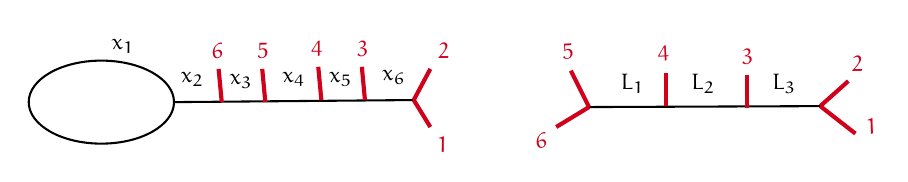
\begin{tikzpicture}[x=0.75pt,y=0.75pt,yscale=-1,xscale=1]
%uncomment if require: \path (0,107); %set diagram left start at 0, and has height of 107

%Shape: Ellipse [id:dp8171192284737407] 
\draw  [line width=0.75]  (39,53) .. controls (39,41.95) and (54.67,33) .. (74,33) .. controls (93.33,33) and (109,41.95) .. (109,53) .. controls (109,64.05) and (93.33,73) .. (74,73) .. controls (54.67,73) and (39,64.05) .. (39,53) -- cycle ;
%Straight Lines [id:da2753604407401631] 
\draw [line width=0.75]    (109,53) -- (224.5,52) ;
%Straight Lines [id:da07842976006769842] 
\draw [color={rgb, 255:red, 208; green, 2; blue, 27 }  ,draw opacity=1 ][line width=1.5]    (132,53) -- (130.5,37) ;
%Straight Lines [id:da4037536630379732] 
\draw [color={rgb, 255:red, 208; green, 2; blue, 27 }  ,draw opacity=1 ][line width=1.5]    (153,53) -- (151.5,37) ;
%Straight Lines [id:da7073042124361943] 
\draw [color={rgb, 255:red, 208; green, 2; blue, 27 }  ,draw opacity=1 ][line width=1.5]    (224.5,52) -- (232.5,37) ;
%Straight Lines [id:da48016913637128567] 
\draw [color={rgb, 255:red, 208; green, 2; blue, 27 }  ,draw opacity=1 ][line width=1.5]    (232.5,65) -- (224.5,52) ;
%Straight Lines [id:da3970174041001511] 
\draw [line width=0.75]    (420.37,54.93) -- (308.97,55.38) ;
%Straight Lines [id:da032293579510118686] 
\draw [color={rgb, 255:red, 208; green, 2; blue, 27 }  ,draw opacity=1 ][line width=1.5]    (308.97,55.38) -- (300.19,37.81) ;
%Straight Lines [id:da2697351076357779] 
\draw [color={rgb, 255:red, 208; green, 2; blue, 27 }  ,draw opacity=1 ][line width=1.5]    (308.97,55.38) -- (293.15,64.99) ;
%Straight Lines [id:da5338676756297784] 
\draw [color={rgb, 255:red, 208; green, 2; blue, 27 }  ,draw opacity=1 ][line width=1.5]    (420.37,54.93) -- (433.88,42.87) ;
%Straight Lines [id:da38033755728152685] 
\draw [color={rgb, 255:red, 208; green, 2; blue, 27 }  ,draw opacity=1 ][line width=1.5]    (420.37,54.93) -- (437.31,68.17) ;
%Straight Lines [id:da2706068472513521] 
\draw [color={rgb, 255:red, 208; green, 2; blue, 27 }  ,draw opacity=1 ][line width=1.5]    (346,55) -- (346,39) ;
%Straight Lines [id:da9743156529492092] 
\draw [color={rgb, 255:red, 208; green, 2; blue, 27 }  ,draw opacity=1 ][line width=1.5]    (385,56) -- (385,40) ;
%Straight Lines [id:da660379227085147] 
\draw [color={rgb, 255:red, 208; green, 2; blue, 27 }  ,draw opacity=1 ][line width=1.5]    (180,52) -- (178.5,36) ;
%Straight Lines [id:da8108668277930373] 
\draw [color={rgb, 255:red, 208; green, 2; blue, 27 }  ,draw opacity=1 ][line width=1.5]    (201,52) -- (199.5,36) ;

% Text Node
\draw (234.5,68.4) node [anchor=north west][inner sep=0.75pt]  [font=\footnotesize,color={rgb, 255:red, 208; green, 2; blue, 27 }  ,opacity=1 ]  {$1$};
% Text Node
\draw (235,23.4) node [anchor=north west][inner sep=0.75pt]  [font=\footnotesize,color={rgb, 255:red, 208; green, 2; blue, 27 }  ,opacity=1 ]  {$2$};
% Text Node
\draw (148,23.4) node [anchor=north west][inner sep=0.75pt]  [font=\footnotesize,color={rgb, 255:red, 208; green, 2; blue, 27 }  ,opacity=1 ]  {$5$};
% Text Node
\draw (126,23.4) node [anchor=north west][inner sep=0.75pt]  [font=\footnotesize,color={rgb, 255:red, 208; green, 2; blue, 27 }  ,opacity=1 ]  {$6$};
% Text Node
\draw (340.74,24.89) node [anchor=north west][inner sep=0.75pt]  [font=\footnotesize,color={rgb, 255:red, 208; green, 2; blue, 27 }  ,opacity=1 ,rotate=-356.58]  {$4$};
% Text Node
\draw (381.17,26.23) node [anchor=north west][inner sep=0.75pt]  [font=\footnotesize,color={rgb, 255:red, 208; green, 2; blue, 27 }  ,opacity=1 ,rotate=-358.17]  {$3$};
% Text Node
\draw (434.28,29.42) node [anchor=north west][inner sep=0.75pt]  [font=\footnotesize,color={rgb, 255:red, 208; green, 2; blue, 27 }  ,opacity=1 ,rotate=-359.91]  {$2$};
% Text Node
\draw (440.88,60.23) node [anchor=north west][inner sep=0.75pt]  [font=\footnotesize,color={rgb, 255:red, 208; green, 2; blue, 27 }  ,opacity=1 ,rotate=-357.22]  {$1$};
% Text Node
\draw (71,17.4) node [anchor=north west][inner sep=0.75pt]  [font=\footnotesize]  {$ \begin{array}{l}
x_{1}\\
\end{array}$};
% Text Node
\draw (111,37.4) node [anchor=north west][inner sep=0.75pt]  [font=\footnotesize]  {$x_{2}$};
% Text Node
\draw (134.5,38.4) node [anchor=north west][inner sep=0.75pt]  [font=\footnotesize]  {$x_{3}$};
% Text Node
\draw (160,37.4) node [anchor=north west][inner sep=0.75pt]  [font=\footnotesize]  {$x_{4}$};
% Text Node
\draw (323,38.4) node [anchor=north west][inner sep=0.75pt]  [font=\footnotesize]  {$L_{1}$};
% Text Node
\draw (294.74,23.89) node [anchor=north west][inner sep=0.75pt]  [font=\footnotesize,color={rgb, 255:red, 208; green, 2; blue, 27 }  ,opacity=1 ,rotate=-356.58]  {$5$};
% Text Node
\draw (281.74,66.89) node [anchor=north west][inner sep=0.75pt]  [font=\footnotesize,color={rgb, 255:red, 208; green, 2; blue, 27 }  ,opacity=1 ,rotate=-356.58]  {$6$};
% Text Node
\draw (357,38.4) node [anchor=north west][inner sep=0.75pt]  [font=\footnotesize]  {$L_{2}$};
% Text Node
\draw (396,38.4) node [anchor=north west][inner sep=0.75pt]  [font=\footnotesize]  {$L_{3}$};
% Text Node
\draw (196,22.4) node [anchor=north west][inner sep=0.75pt]  [font=\footnotesize,color={rgb, 255:red, 208; green, 2; blue, 27 }  ,opacity=1 ]  {$3$};
% Text Node
\draw (174,22.4) node [anchor=north west][inner sep=0.75pt]  [font=\footnotesize,color={rgb, 255:red, 208; green, 2; blue, 27 }  ,opacity=1 ]  {$4$};
% Text Node
\draw (182.5,37.4) node [anchor=north west][inner sep=0.75pt]  [font=\footnotesize]  {$x_{5}$};
% Text Node
\draw (208,36.4) node [anchor=north west][inner sep=0.75pt]  [font=\footnotesize]  {$x_{6}$};


\end{tikzpicture}
    \caption{The point $p$ in $\Mgn{1,6}^\trop \times \Mgn{0,6}^\trop$. We have $x_1<<x_2<<x_3<<x_4<<x_5<<x_6<<L_1<<L_2<<L_3$.}
    \label{fig:l=1g=1image}
\end{figure}

We start constructing $\Gamma $ and $T$ by creating the genus zero part, containing the marked points. Due to the cover being degree 3, there will be one edge cutting from the active edge to end with a transposition and at most one edge joining the active edge, because the genus could be degree 2 or 3. Therefore, we have three options for the genus zero part of $\Gamma$, shown in Figure \ref{fig:g=1cutjoin}. 
\begin{figure}[tb]
    \centering


\tikzset{every picture/.style={line width=0.75pt}} %set default line width to 0.75pt        

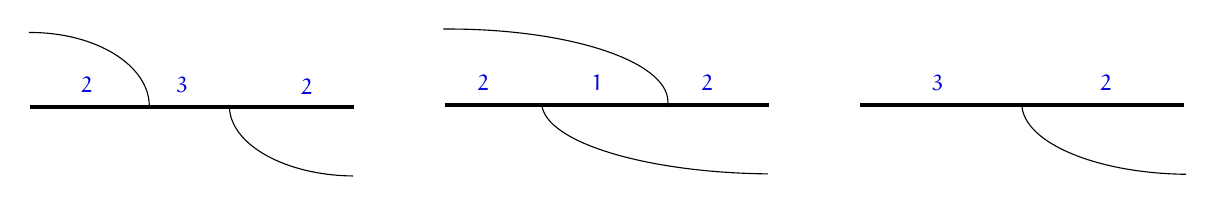
\begin{tikzpicture}[x=0.75pt,y=0.75pt,yscale=-1,xscale=1]
%uncomment if require: \path (0,109); %set diagram left start at 0, and has height of 109

%Straight Lines [id:da314248435223343] 
\draw [line width=1.5]    (24.5,51) -- (180.5,51) ;
%Straight Lines [id:da5087164244479825] 
\draw [line width=1.5]    (224.5,50) -- (380.5,50) ;
%Straight Lines [id:da7941105153730301] 
\draw [line width=1.5]    (424.5,50) -- (580.5,50) ;
%Shape: Arc [id:dp41352026855074664] 
\draw  [draw opacity=0] (24.08,15.22) .. controls (24.14,15.22) and (24.2,15.22) .. (24.26,15.22) .. controls (56.08,15.01) and (81.98,30.86) .. (82.11,50.62) .. controls (82.11,51.08) and (82.1,51.54) .. (82.08,51.99) -- (24.5,51) -- cycle ; \draw   (24.08,15.22) .. controls (24.14,15.22) and (24.2,15.22) .. (24.26,15.22) .. controls (56.08,15.01) and (81.98,30.86) .. (82.11,50.62) .. controls (82.11,51.08) and (82.1,51.54) .. (82.08,51.99) ;  
%Shape: Arc [id:dp3239163769655016] 
\draw  [draw opacity=0] (223.83,13.55) .. controls (223.89,13.55) and (223.95,13.55) .. (224.01,13.55) .. controls (283.51,13.16) and (331.86,28.86) .. (331.99,48.62) .. controls (331.99,49.48) and (331.91,50.34) .. (331.73,51.19) -- (224.25,49.33) -- cycle ; \draw   (223.83,13.55) .. controls (223.89,13.55) and (223.95,13.55) .. (224.01,13.55) .. controls (283.51,13.16) and (331.86,28.86) .. (331.99,48.62) .. controls (331.99,49.48) and (331.91,50.34) .. (331.73,51.19) ;  
%Shape: Arc [id:dp38030440410803235] 
\draw  [draw opacity=0] (180.15,84.34) .. controls (147.48,84.01) and (121.09,69.14) .. (120.7,51) -- (180.5,51) -- cycle ; \draw   (180.15,84.34) .. controls (147.48,84.01) and (121.09,69.14) .. (120.7,51) ;  
%Shape: Arc [id:dp8414802740112062] 
\draw  [draw opacity=0] (380.15,83.34) .. controls (320.96,82.76) and (272.9,67.93) .. (271.23,50) -- (380.5,50) -- cycle ; \draw   (380.15,83.34) .. controls (320.96,82.76) and (272.9,67.93) .. (271.23,50) ;  
%Shape: Arc [id:dp8869474448581858] 
\draw  [draw opacity=0] (581.63,83.53) .. controls (538.36,83.1) and (503.32,68.25) .. (502.51,50.19) -- (581.99,50.19) -- cycle ; \draw   (581.63,83.53) .. controls (538.36,83.1) and (503.32,68.25) .. (502.51,50.19) ;  

% Text Node
\draw (48,35.4) node [anchor=north west][inner sep=0.75pt]  [font=\footnotesize,color={rgb, 255:red, 0; green, 0; blue, 223 }  ,opacity=1 ]  {$2$};
% Text Node
\draw (94,35.4) node [anchor=north west][inner sep=0.75pt]  [font=\footnotesize,color={rgb, 255:red, 0; green, 0; blue, 223 }  ,opacity=1 ]  {$3$};
% Text Node
\draw (154,36.4) node [anchor=north west][inner sep=0.75pt]  [font=\footnotesize,color={rgb, 255:red, 0; green, 0; blue, 223 }  ,opacity=1 ]  {$2$};
% Text Node
\draw (239,34.4) node [anchor=north west][inner sep=0.75pt]  [font=\footnotesize,color={rgb, 255:red, 0; green, 0; blue, 223 }  ,opacity=1 ]  {$2$};
% Text Node
\draw (347,34.4) node [anchor=north west][inner sep=0.75pt]  [font=\footnotesize,color={rgb, 255:red, 0; green, 0; blue, 223 }  ,opacity=1 ]  {$2$};
% Text Node
\draw (294,34.4) node [anchor=north west][inner sep=0.75pt]  [font=\footnotesize,color={rgb, 255:red, 0; green, 0; blue, 223 }  ,opacity=1 ]  {$1$};
% Text Node
\draw (539,34.4) node [anchor=north west][inner sep=0.75pt]  [font=\footnotesize,color={rgb, 255:red, 0; green, 0; blue, 223 }  ,opacity=1 ]  {$2$};
% Text Node
\draw (458,34.4) node [anchor=north west][inner sep=0.75pt]  [font=\footnotesize,color={rgb, 255:red, 0; green, 0; blue, 223 }  ,opacity=1 ]  {$3$};


\end{tikzpicture}
    \caption{The three options for a genus zero graph containing one cut and at most one join.}
    \label{fig:g=1cutjoin}
\end{figure}

When placing marked points on the options for $\Gamma$, there are three $L_i$'s, therefore three lengths need to be free to be made long. The marked point fragments shown in \ref{fig:l=1g=1frags} each have 3 vertical lengths that when placed correctly on a cover, will allow for the three $L_i$'s to be made long. The fragment on the left hand side requires a cover with 3 edges on the left hand side covering the tree with three marked points and it needs 2 edges covering the tree on the right hand side. Therefore, the fragment on the left side of Figure \ref{fig:l=1g=1frags} can be placed on the genus zero graph in the middle of Figure \ref{fig:g=1cutjoin}. Similarly, the fragment on the right hand side of Figure \ref{fig:l=1g=1frags} can only be placed on the graph on the left of Figure \ref{fig:g=1cutjoin}. Therefore, the rightmost graph in Figure \ref{fig:g=1cutjoin} does not contribute.

\begin{figure}[tb]
    \centering


\tikzset{every picture/.style={line width=0.75pt}} %set default line width to 0.75pt        

\begin{tikzpicture}[x=0.75pt,y=0.75pt,yscale=-1,xscale=1]
%uncomment if require: \path (0,103); %set diagram left start at 0, and has height of 103

%Straight Lines [id:da7767776511996656] 
\draw    (48.81,50.09) -- (48.81,79.33) ;
%Straight Lines [id:da24637572827038867] 
\draw [color={rgb, 255:red, 208; green, 2; blue, 27 }  ,draw opacity=1 ]   (48.81,50.09) -- (56.94,33.03) ;
%Straight Lines [id:da7286866024439065] 
\draw [color={rgb, 255:red, 208; green, 2; blue, 27 }  ,draw opacity=1 ]   (42.3,33.03) -- (48.81,50.09) ;
%Straight Lines [id:da1822946868848161] 
\draw [color={rgb, 255:red, 208; green, 2; blue, 27 }  ,draw opacity=1 ]   (49.6,62.7) -- (64.25,62.7) ;
%Straight Lines [id:da2502412591973977] 
\draw [color={rgb, 255:red, 208; green, 2; blue, 27 }  ,draw opacity=1 ]   (84.47,77.32) -- (85.27,59.2) ;
%Straight Lines [id:da06260770495677015] 
\draw    (106.1,49.08) -- (106.1,78.33) ;
%Straight Lines [id:da16312187620988272] 
\draw [color={rgb, 255:red, 208; green, 2; blue, 27 }  ,draw opacity=1 ]   (106.1,49.08) -- (114.24,32.02) ;
%Straight Lines [id:da3390981476012074] 
\draw [color={rgb, 255:red, 208; green, 2; blue, 27 }  ,draw opacity=1 ]   (99.59,32.02) -- (106.1,49.08) ;
%Straight Lines [id:da026156978518896867] 
\draw    (189.87,50.91) -- (189.87,79) ;
%Straight Lines [id:da9810195831589976] 
\draw [color={rgb, 255:red, 208; green, 2; blue, 27 }  ,draw opacity=1 ]   (189.87,50.91) -- (196.92,34.53) ;
%Straight Lines [id:da9353261081993685] 
\draw [color={rgb, 255:red, 208; green, 2; blue, 27 }  ,draw opacity=1 ]   (184.22,34.53) -- (189.87,50.91) ;
%Straight Lines [id:da5166326240133854] 
\draw [color={rgb, 255:red, 208; green, 2; blue, 27 }  ,draw opacity=1 ]   (240.48,63.99) -- (253.17,63.99) ;
%Straight Lines [id:da2622698732150959] 
\draw [color={rgb, 255:red, 208; green, 2; blue, 27 }  ,draw opacity=1 ]   (214.89,79) -- (215.58,61.6) ;
%Straight Lines [id:da4383465905285655] 
\draw    (240.48,50.91) -- (240.48,79) ;
%Straight Lines [id:da1233537404466527] 
\draw [color={rgb, 255:red, 208; green, 2; blue, 27 }  ,draw opacity=1 ]   (240.48,50.91) -- (247.53,34.53) ;
%Straight Lines [id:da2549860695827755] 
\draw [color={rgb, 255:red, 208; green, 2; blue, 27 }  ,draw opacity=1 ]   (234.83,34.53) -- (240.48,50.91) ;

% Text Node
\draw (67.22,59.21) node [anchor=north west][inner sep=0.75pt]  [font=\tiny,color={rgb, 255:red, 208; green, 2; blue, 27 }  ,opacity=1 ]  {$4$};
% Text Node
\draw (60.85,21.46) node [anchor=north west][inner sep=0.75pt]  [font=\tiny,color={rgb, 255:red, 208; green, 2; blue, 27 }  ,opacity=1 ]  {$5$};
% Text Node
\draw (34.59,20.96) node [anchor=north west][inner sep=0.75pt]  [font=\tiny,color={rgb, 255:red, 208; green, 2; blue, 27 }  ,opacity=1 ]  {$6$};
% Text Node
\draw (83.93,47.13) node [anchor=north west][inner sep=0.75pt]  [font=\tiny,color={rgb, 255:red, 208; green, 2; blue, 27 }  ,opacity=1 ]  {$3$};
% Text Node
\draw (118.14,20.45) node [anchor=north west][inner sep=0.75pt]  [font=\tiny,color={rgb, 255:red, 208; green, 2; blue, 27 }  ,opacity=1 ]  {$1$};
% Text Node
\draw (91.89,19.95) node [anchor=north west][inner sep=0.75pt]  [font=\tiny,color={rgb, 255:red, 208; green, 2; blue, 27 }  ,opacity=1 ]  {$2$};
% Text Node
\draw (212.24,47.97) node [anchor=north west][inner sep=0.75pt]  [font=\tiny,color={rgb, 255:red, 208; green, 2; blue, 27 }  ,opacity=1 ]  {$4$};
% Text Node
\draw (199.51,23.31) node [anchor=north west][inner sep=0.75pt]  [font=\tiny,color={rgb, 255:red, 208; green, 2; blue, 27 }  ,opacity=1 ]  {$5$};
% Text Node
\draw (176.74,22.83) node [anchor=north west][inner sep=0.75pt]  [font=\tiny,color={rgb, 255:red, 208; green, 2; blue, 27 }  ,opacity=1 ]  {$6$};
% Text Node
\draw (256.33,58.6) node [anchor=north west][inner sep=0.75pt]  [font=\tiny,color={rgb, 255:red, 208; green, 2; blue, 27 }  ,opacity=1 ]  {$3$};
% Text Node
\draw (250.12,23.31) node [anchor=north west][inner sep=0.75pt]  [font=\tiny,color={rgb, 255:red, 208; green, 2; blue, 27 }  ,opacity=1 ]  {$1$};
% Text Node
\draw (227.35,22.83) node [anchor=north west][inner sep=0.75pt]  [font=\tiny,color={rgb, 255:red, 208; green, 2; blue, 27 }  ,opacity=1 ]  {$2$};


\end{tikzpicture}
    \caption{Two configurations of marked points that allow for three long edges to be forgotten in the stabilization of the cover curve.}
    \label{fig:l=1g=1frags}
\end{figure}

The genus zero part of the $\Gamma \to T$s that we are constructing both use three transpositions, and the Riemann-Hurwitz formula gives that there are $6$ transpositions total, therefore we have 3 transpositions left to create $\gGamma \to \gT$. There is a unique way to form a loop with 3 transpositions. Putting this loop together with the genus zero parts discussed above, we can now place the marked fragments on $\Gamma$ and $T$. 

For one cover, start with a simple loop using three transpositions, then have an edge cut from the active edge at a distance of $y_2$ away from the loop. Next, have an edge join the active edge at a distance of $y_3+y_4$ to the right of the cutting edge. Looking at $T_1$, place a tree with three marked points to the right $y_3$ from the fourth transposition. There are three trees in $\Gamma_1$ covering this tree in $T_1$. Place the marked point 6 at the end of the tree on the edge cutting from the active edge covering $T_1$, then place the marked point 5 at the end of the tree on the active edge. On the tree lying on the edge joining the active edge, place the marked point 4 at the distance $y_6$ down from 5 and 6. Moving to the right, place the marked point 3 at $y_7$ away from the edge joining, then $y_8$ to the right, place the marked points 1 and 2 on separate trees of length $y_9$. 

Place the points in a similar way for $\Gamma_2 \to T_2$, but with the cut and join switched. Together, we have the two covers shown in Figure \ref{fig:l=1g=1}.
\begin{figure}[tb]
    \centering
    \inputTikZ{.8\textwidth}{Figures/l=1g=1}
    \caption{The two covers in $((\Fs\times\Ft))^{-1}(p)$ for $\ell=1$ and $g=1$.}
    \label{fig:l=1g=1}
\end{figure}

We now compute the local degree of $(\Fs\times\Ft)$ at these inverse images, which gives us the multiplicities which we need to count the covers. The multiplicity of the inverse image is the product of three factors: an automorphism factor, a product of local Hurwitz numbers and a dilation factor corresponding to the determinant of the matrix representing the map $\Fs\times\Ft$. 

To calculate the local Hurwitz numbers for cover 1, every vertex in $\Gamma_1$ is either trivalent with degree one edges in all directions or two edges of degree 2 in different directions and 2 edges of degree 1 in the same direction. Both of these types of vertices have local Hurwitz number equal to 1, therefore the product of all local Hurwitz numbers is 1. Additionally, $\Gamma_2$ contains vertices with an edge of degree 3 in one direction and simple transpositions in the other 2 directions, as well as a vertex with two directions containing an edge of degree 3 and three edges of degree 1 in the third direction. The first of these vertex options has local Hurwitz number equal to 1. The second option, we are marking one of the edges of degree 1, so the local Hurwitz number is also equal to 1. All together, the product of local Hurwitz numbers is equal to 1. 

For each cover, we have one factor of 2 corresponding to switching simultaneously the two unlabeled left ends of branching type $2$ and their inverse images. Also, a second factor of 2 consists of switching the two degree $1$ edges of $\Gamma_i$ forming the loop. However, this is also a nontrivial automorphism of $\overline{\Gamma_i}$. Altogether, we have
\begin{equation}
    \frac{|\Aut(\overline{\Gamma_i})|}{|\Aut(\phi_i)|} = \frac{1}{2}.
\end{equation}


To calculate the dilation factors, we set up the following matrices representing the $x_i$'s and $L_j$'s in terms of the $y_k$'s: 
 {\scriptsize
\[\begin{array}[t]{cc}
  M_1=\begin{blockarray}{cccccccccc}
   &y_1 & y_2 & y_3 & y_4 & y_5 & y_6 & y_7 & y_8 & y_9\\
    \begin{block}{c[ccccccccc]}
      x_1 & 2 & 0 & 0 & 0 & 0 & 0 & 0 & 0 & 0\\
      x_2 & 0 & 1 & 0 & 0 & 0 & 0 & 0 & 0 & 0\\
      x_3 & 0 & 0 & 1 & 0 & 0 & 0 & 0 & 0 & 0\\
      x_4 & 0 & 0 & 0 & 1 & 0 & 0 & 0 & 0 & 0\\
      x_5 & 0 & 0 & 0 & 0 & 0 & 0 & 1 & 0 & 0\\
      x_6 & 0 & 0 & 0 & 0 & 0 & 0 & 0 & 1 & 0\\
      L_1 & 0 & 0 & 0 & 0 & 0 & 1 & 0 & 0 & 0\\
      L_2 & 0 & 0 & 0 & 1 & 1 & 0 & 2 & 0 & 0\\
      L_3 & 0 & 0 & 0 & 0 & 0 & 0 & 0 & 2 & 1\\
    \end{block}
  \end{blockarray} \\
 M_2=\begin{blockarray}{cccccccccc}
   &y'_1 & y'_2 & y'_3 & y'_4 & y'_5 & y'_6 & y'_7 & y'_8 & y'_9\\
    \begin{block}{c[ccccccccc]}
      x_1 & 2 & 0 & 0 & 0 & 0 & 0 & 0 & 0 & 0\\
      x_2 & 0 & 1 & 0 & 0 & 0 & 0 & 0 & 0 & 0\\
      x_3 & 0 & 0 & 1 & 0 & 0 & 0 & 0 & 0 & 0\\
      x_4 & 0 & 0 & 0 & 0 & 1 & 0 & 0 & 0 & 0\\
      x_5 & 0 & 0 & 0 & 0 & 0 & 1 & 0 & 0 & 0\\
      x_6 & 0 & 0 & 0 & 0 & 0 & 0 & 1 & 0 & 0\\
      L_1 & 0 & 0 & 2 & 1 & 3 & 0 & 0 & 0 & 0\\
      L_2 & 0 & 0 & 0 & 0 & 0 & 3 & 2 & 1 & 0\\
      L_3 & 0 & 0 & 0 & 0 & 0 & 0 & 0 & 0 & 1\\
    \end{block}
  \end{blockarray}
  \end{array}
\]
}
We see that $|\det M_i |=2$ for $i = 1,2$.
All together the multiplicity of each cover in $(\Fs\times\Ft)^{-1}(p)$ is $1\cdot \frac{1}{2}\cdot 2=1$. Since we have two inverse images each with multiplicity one,  we obtain $\Tev^\trop_{1,1} = 2$.

Next, looking at $g=2$, there are 4 preimages as shown in Figure \ref{fig:l=1g=2}, each with multiplicity 1, so $\Tev_{2,1}^\trop=4$.
\begin{figure}[tb]
    \centering


\tikzset{every picture/.style={line width=0.75pt}} %set default line width to 0.75pt        

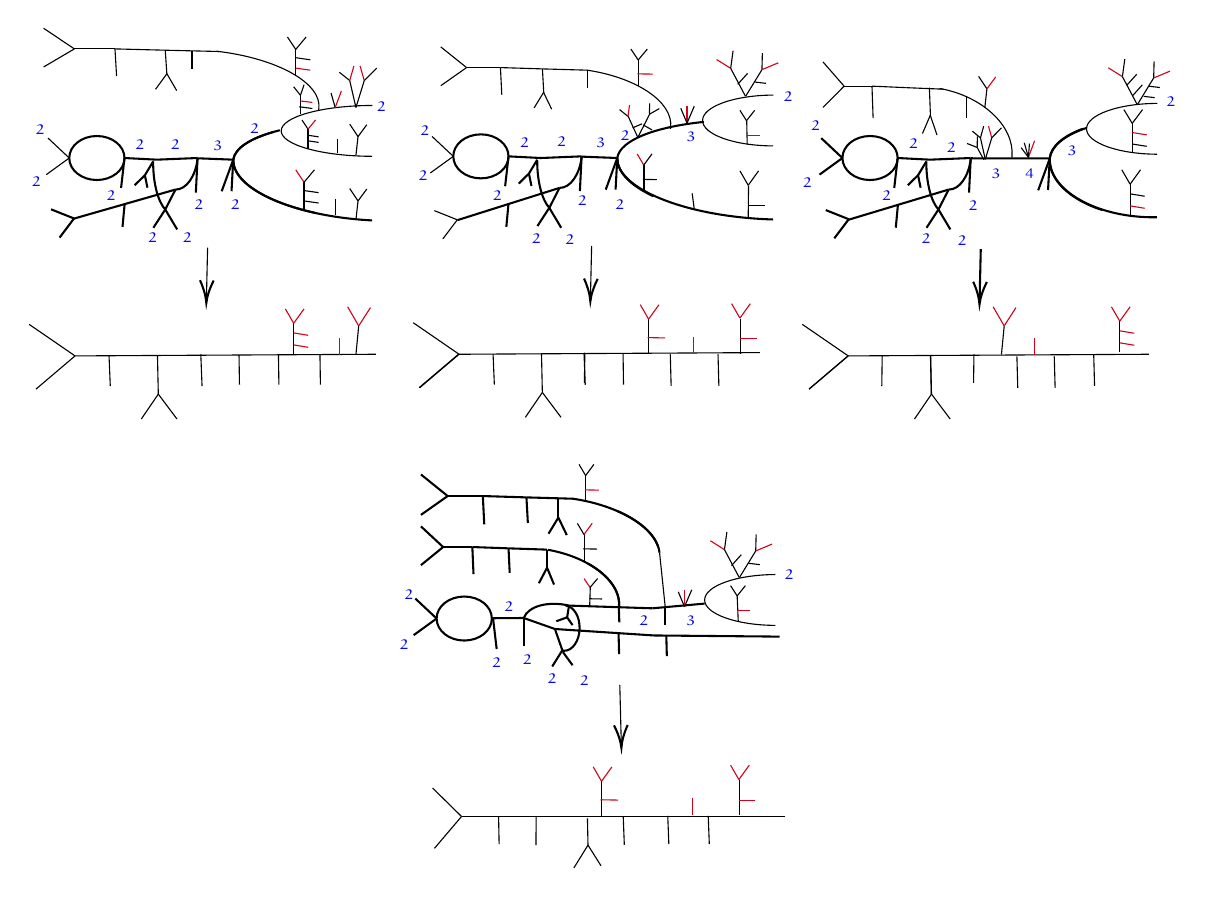
\begin{tikzpicture}[x=0.75pt,y=0.75pt,yscale=-1,xscale=1]
%uncomment if require: \path (0,480); %set diagram left start at 0, and has height of 480

%Straight Lines [id:da05122462230143654] 
\draw    (32.67,201.67) -- (177.58,200.87) ;
%Straight Lines [id:da895168427904524] 
\draw    (32.67,201.67) -- (10.56,186.47) ;
%Straight Lines [id:da31800838995746816] 
\draw    (32.67,201.67) -- (13.84,217.67) ;
%Straight Lines [id:da5731671037982771] 
\draw    (49.04,201.67) -- (49.65,216.27) ;
%Straight Lines [id:da8169612972850104] 
\draw    (72.37,201.27) -- (72.78,220.07) ;
%Straight Lines [id:da06332615933468722] 
\draw    (93.25,200.87) -- (93.86,216.27) ;
%Straight Lines [id:da536384139330697] 
\draw    (111.67,201.27) -- (111.88,215.47) ;
%Straight Lines [id:da2800233209446439] 
\draw    (19.64,96.72) -- (29.88,106.32) ;
%Straight Lines [id:da9430418310597888] 
\draw    (29.88,106.32) -- (18.82,114.32) ;
%Shape: Ellipse [id:dp9995507342509742] 
\draw  [line width=0.75]  (29.88,106.32) .. controls (29.88,100.46) and (35.83,95.72) .. (43.18,95.72) .. controls (50.53,95.72) and (56.49,100.46) .. (56.49,106.32) .. controls (56.49,112.17) and (50.53,116.92) .. (43.18,116.92) .. controls (35.83,116.92) and (29.88,112.17) .. (29.88,106.32) -- cycle ;
%Straight Lines [id:da9915089548344329] 
\draw [line width=0.75]    (56.49,106.32) -- (54.85,120.72) ;
%Straight Lines [id:da04601550566192891] 
\draw [line width=0.75]    (56.49,106.32) -- (72.04,107.12) ;
%Straight Lines [id:da8826675526266912] 
\draw    (72.78,220.07) -- (81.79,232.07) ;
%Straight Lines [id:da690814656628189] 
\draw    (72.78,220.07) -- (64.6,232.07) ;
%Straight Lines [id:da4158715286050403] 
\draw [line width=0.75]    (32.06,135.54) -- (81.05,121.52) ;
%Straight Lines [id:da7794010774979205] 
\draw [line width=0.75]    (32.18,135.45) -- (21.13,131.05) ;
%Straight Lines [id:da9907325880206637] 
\draw [line width=0.75]    (32.18,135.45) -- (25.22,144.65) ;
%Straight Lines [id:da5863982048911034] 
\draw [line width=0.75]    (56.55,128.53) -- (55.53,139.53) ;
%Straight Lines [id:da3532076114014613] 
\draw [line width=0.75]    (81.05,121.52) -- (76.13,131.12) ;
%Straight Lines [id:da9621975692699847] 
\draw [line width=0.75]    (76.13,131.12) -- (70.4,139.92) ;
%Straight Lines [id:da6801555166743909] 
\draw [line width=0.75]    (76.13,131.12) -- (81.87,140.72) ;
%Straight Lines [id:da7496788388360165] 
\draw [line width=0.75]    (72.04,107.12) -- (91.69,106.32) ;
%Shape: Arc [id:dp7192816333090397] 
\draw  [draw opacity=0][line width=0.75]  (91.72,106.51) .. controls (90.78,115.1) and (86.3,121.62) .. (81.05,121.52) .. controls (81.05,121.52) and (81.05,121.52) .. (81.05,121.52) -- (81.4,103.6) -- cycle ; \draw  [line width=0.75]  (91.72,106.51) .. controls (90.78,115.1) and (86.3,121.62) .. (81.05,121.52) .. controls (81.05,121.52) and (81.05,121.52) .. (81.05,121.52) ;  
%Straight Lines [id:da9733095163881604] 
\draw [line width=0.75]    (91.69,106.32) -- (90.87,123.02) ;
%Straight Lines [id:da25058054978981703] 
\draw [line width=0.75]    (91.72,106.45) -- (108.88,107.12) ;
%Straight Lines [id:da65858984812399] 
\draw [line width=0.75]    (108.88,107.12) -- (108.06,122.32) ;
%Shape: Arc [id:dp4632137558256588] 
\draw  [draw opacity=0][line width=0.75]  (175.8,136.39) .. controls (138.29,134.46) and (108.52,121.45) .. (108.88,107.13) -- (177.81,110.15) -- cycle ; \draw  [line width=0.75]  (175.8,136.39) .. controls (138.29,134.46) and (108.52,121.45) .. (108.88,107.13) ;  
%Shape: Arc [id:dp5172417584798175] 
\draw  [draw opacity=0][line width=0.75]  (76.21,131.19) .. controls (72.74,127.55) and (70.3,118.75) .. (70.3,108.48) .. controls (70.3,108.3) and (70.3,108.13) .. (70.3,107.96) -- (79.78,108.48) -- cycle ; \draw  [line width=0.75]  (76.21,131.19) .. controls (72.74,127.55) and (70.3,118.75) .. (70.3,108.48) .. controls (70.3,108.3) and (70.3,108.13) .. (70.3,107.96) ;  
%Shape: Arc [id:dp7681279435503876] 
\draw  [draw opacity=0][line width=0.75]  (108.89,107.11) .. controls (109.65,101.63) and (116.93,96.98) .. (128.42,93.72) -- (182.87,111.4) -- cycle ; \draw  [line width=0.75]  (108.89,107.11) .. controls (109.65,101.63) and (116.93,96.98) .. (128.42,93.72) ;  
%Straight Lines [id:da5769692743866277] 
\draw    (96.53,149.51) -- (95.96,174.21) ;
\draw [shift={(95.91,176.21)}, rotate = 271.32] [color={rgb, 255:red, 0; green, 0; blue, 0 }  ][line width=0.75]    (10.93,-3.29) .. controls (6.95,-1.4) and (3.31,-0.3) .. (0,0) .. controls (3.31,0.3) and (6.95,1.4) .. (10.93,3.29)   ;
%Straight Lines [id:da7033612942192056] 
\draw [line width=0.75]    (70.3,107.97) -- (66.31,114.62) ;
%Straight Lines [id:da23423196203212404] 
\draw [line width=0.75]    (66.31,114.62) -- (67.54,120.62) ;
%Straight Lines [id:da279154632501033] 
\draw [line width=0.75]    (66.31,114.62) -- (61.4,119.42) ;
%Straight Lines [id:da5407125907587447] 
\draw    (218.87,423.57) -- (374.68,423.57) ;
%Straight Lines [id:da9593619371341235] 
\draw    (204.95,409.87) -- (218.87,423.57) ;
%Straight Lines [id:da5770667699653664] 
\draw    (205.82,438.93) -- (218.87,423.57) ;
%Straight Lines [id:da4120985341094361] 
\draw    (236.98,436.86) -- (236.72,423.41) ;
%Straight Lines [id:da32289798950094384] 
\draw    (254.74,437.36) -- (254.82,423.74) ;
%Straight Lines [id:da9811843340153472] 
\draw    (279.8,437.36) -- (279.54,424.49) ;
%Straight Lines [id:da03427071927984149] 
\draw    (279.8,437.36) -- (286.07,447.32) ;
%Straight Lines [id:da6749942745792021] 
\draw    (273.02,448.32) -- (279.8,437.36) ;
%Straight Lines [id:da5929832699549258] 
\draw    (296.78,423.57) -- (297.3,437.19) ;
%Straight Lines [id:da006360558155229734] 
\draw [line width=0.75]    (234.06,328.05) -- (235.8,342.89) ;
%Straight Lines [id:da36250505346187856] 
\draw [line width=0.75]    (234.06,328.05) -- (248.85,327.94) ;
%Straight Lines [id:da015582605528720483] 
\draw [line width=0.75]    (248.85,327.94) -- (248.85,341.33) ;
%Shape: Arc [id:dp22994046189221584] 
\draw  [draw opacity=0][line width=0.75]  (248.86,327.92) .. controls (250.91,322.3) and (260.38,319.63) .. (270.58,321.94) .. controls (270.6,321.95) and (270.63,321.95) .. (270.66,321.96) -- (267.83,332.94) -- cycle ; \draw  [line width=0.75]  (248.86,327.92) .. controls (250.91,322.3) and (260.38,319.63) .. (270.58,321.94) .. controls (270.6,321.95) and (270.63,321.95) .. (270.66,321.96) ;  
%Straight Lines [id:da5613314763526169] 
\draw [line width=0.75]    (248.85,327.94) -- (263.87,333.24) ;
%Straight Lines [id:da13570458806469854] 
\draw [line width=0.75]    (263.87,333.24) -- (267.79,344.45) ;
%Shape: Arc [id:dp23328025206676184] 
\draw  [draw opacity=0][line width=0.75]  (269.07,321.93) .. controls (272.88,322.32) and (275.84,327.1) .. (275.76,332.91) .. controls (275.68,338.93) and (272.36,343.78) .. (268.33,343.74) .. controls (268.01,343.73) and (267.7,343.7) .. (267.39,343.64) -- (268.47,332.82) -- cycle ; \draw  [line width=0.75]  (269.07,321.93) .. controls (272.88,322.32) and (275.84,327.1) .. (275.76,332.91) .. controls (275.68,338.93) and (272.36,343.78) .. (268.33,343.74) .. controls (268.01,343.73) and (267.7,343.7) .. (267.39,343.64) ;  
%Straight Lines [id:da41678636694136917] 
\draw [line width=0.75]    (267.35,343.63) -- (262.56,351.3) ;
%Straight Lines [id:da6641291356913159] 
\draw [line width=0.75]    (267.79,344.45) -- (272.36,350.67) ;
%Straight Lines [id:da8715646414355216] 
\draw [line width=0.75]    (263.87,333.24) -- (311.53,336.35) ;
%Straight Lines [id:da5465952153155238] 
\draw [line width=0.75]    (270.67,321.96) -- (310.87,323.27) ;
%Straight Lines [id:da822055640865774] 
\draw [line width=0.75]    (210.01,293.75) -- (199.32,302.47) ;
%Straight Lines [id:da9550217007708093] 
\draw [line width=0.75]    (199.32,283.79) -- (210.01,293.75) ;
%Straight Lines [id:da23033369936687587] 
\draw [line width=0.75]    (210.01,293.75) -- (224.08,293.75) ;
%Straight Lines [id:da6054317152422648] 
\draw [line width=0.75]    (224.08,293.75) -- (224.64,306.83) ;
%Straight Lines [id:da38966950950911317] 
\draw [line width=0.75]    (224.08,293.75) -- (241.52,294.38) ;
%Straight Lines [id:da8370257837157022] 
\draw [line width=0.75]    (241.52,294.38) -- (242.08,306.21) ;
%Straight Lines [id:da6173448765407092] 
\draw [line width=0.75]    (241.52,294.38) -- (260.08,295) ;
%Straight Lines [id:da06828753334125337] 
\draw [line width=0.75]    (260.08,295) -- (260.08,303.72) ;
%Straight Lines [id:da34828136411973487] 
\draw [line width=0.75]    (260.08,303.72) -- (263.45,311.82) ;
%Straight Lines [id:da6826559186757841] 
\draw [line width=0.75]    (260.08,303.72) -- (256.14,311.19) ;
%Straight Lines [id:da3610649907582577] 
\draw [line width=0.75]    (270.67,321.96) -- (269.74,327.63) ;
%Straight Lines [id:da4277121572863143] 
\draw [line width=0.75]    (269.74,327.63) -- (264.52,329.5) ;
%Straight Lines [id:da5080682872804914] 
\draw [line width=0.75]    (269.74,327.63) -- (272.36,331.37) ;
%Shape: Arc [id:dp2706718045019485] 
\draw  [draw opacity=0][line width=0.75]  (260.47,295.07) .. controls (280.86,298.69) and (295.91,310.51) .. (294.74,322.57) .. controls (294.72,322.78) and (294.7,322.99) .. (294.67,323.2) -- (254.09,317.75) -- cycle ; \draw  [line width=0.75]  (260.47,295.07) .. controls (280.86,298.69) and (295.91,310.51) .. (294.74,322.57) .. controls (294.72,322.78) and (294.7,322.99) .. (294.67,323.2) ;  
%Straight Lines [id:da7047688305349695] 
\draw [line width=0.75]    (294.67,323.18) -- (294.9,330.06) ;
%Straight Lines [id:da20352239959165708] 
\draw [line width=0.75]    (294.53,335.35) -- (294.79,345.31) ;
%Straight Lines [id:da9708595681556909] 
\draw [line width=0.75]    (311.53,336.35) -- (372.11,336.91) ;
%Straight Lines [id:da8784583625486153] 
\draw    (295.12,360.12) -- (295.85,388.51) ;
\draw [shift={(295.9,390.51)}, rotate = 268.52] [color={rgb, 255:red, 0; green, 0; blue, 0 }  ][line width=0.75]    (10.93,-3.29) .. controls (6.95,-1.4) and (3.31,-0.3) .. (0,0) .. controls (3.31,0.3) and (6.95,1.4) .. (10.93,3.29)   ;
%Straight Lines [id:da914104212945104] 
\draw    (217.69,200.87) -- (362.61,200.07) ;
%Straight Lines [id:da5347433695659032] 
\draw    (217.69,200.87) -- (195.59,185.67) ;
%Straight Lines [id:da6159741875417273] 
\draw    (217.69,200.87) -- (198.86,216.87) ;
%Straight Lines [id:da2962031804626746] 
\draw    (234.07,200.87) -- (234.68,215.47) ;
%Straight Lines [id:da128554816610855] 
\draw    (257.4,200.47) -- (257.81,219.27) ;
%Straight Lines [id:da3881560603131846] 
\draw    (278.28,200.07) -- (278.07,214.67) ;
%Straight Lines [id:da12039153156932869] 
\draw    (296.7,200.47) -- (296.91,215.47) ;
%Straight Lines [id:da5099376435477123] 
\draw    (204.67,95.92) -- (214.91,105.52) ;
%Straight Lines [id:da8004745620730198] 
\draw    (214.91,105.52) -- (203.85,113.52) ;
%Shape: Ellipse [id:dp7112128699419575] 
\draw  [line width=0.75]  (214.91,105.52) .. controls (214.91,99.66) and (220.86,94.92) .. (228.21,94.92) .. controls (235.56,94.92) and (241.51,99.66) .. (241.51,105.52) .. controls (241.51,111.37) and (235.56,116.12) .. (228.21,116.12) .. controls (220.86,116.12) and (214.91,111.37) .. (214.91,105.52) -- cycle ;
%Straight Lines [id:da9792600275415637] 
\draw [line width=0.75]    (241.51,105.52) -- (239.88,119.92) ;
%Straight Lines [id:da18778687561308782] 
\draw [line width=0.75]    (241.51,105.52) -- (257.07,106.32) ;
%Straight Lines [id:da4877797022877657] 
\draw    (257.81,219.27) -- (266.82,231.27) ;
%Straight Lines [id:da9463079862998041] 
\draw    (257.81,219.27) -- (249.62,231.27) ;
%Straight Lines [id:da05865591839080064] 
\draw [line width=0.75]    (216.89,136.26) -- (266.08,120.72) ;
%Straight Lines [id:da19646237001514955] 
\draw    (216.84,136.08) -- (205.79,131.68) ;
%Straight Lines [id:da8030769754425777] 
\draw    (216.84,136.08) -- (209.88,145.28) ;
%Straight Lines [id:da09194754451988585] 
\draw [line width=0.75]    (241.48,128.49) -- (240.46,139.49) ;
%Straight Lines [id:da04337463575456435] 
\draw [line width=0.75]    (266.08,120.72) -- (261.16,130.32) ;
%Straight Lines [id:da8422397128566506] 
\draw [line width=0.75]    (261.16,130.32) -- (255.43,139.12) ;
%Straight Lines [id:da49432511722969963] 
\draw [line width=0.75]    (261.16,130.32) -- (266.89,139.92) ;
%Straight Lines [id:da040443258031210405] 
\draw [line width=0.75]    (257.07,106.32) -- (276.72,105.52) ;
%Shape: Arc [id:dp9375473879432219] 
\draw  [draw opacity=0][line width=0.75]  (276.75,105.71) .. controls (275.81,114.3) and (271.33,120.82) .. (266.08,120.72) .. controls (266.08,120.72) and (266.08,120.72) .. (266.08,120.72) -- (266.43,102.8) -- cycle ; \draw  [line width=0.75]  (276.75,105.71) .. controls (275.81,114.3) and (271.33,120.82) .. (266.08,120.72) .. controls (266.08,120.72) and (266.08,120.72) .. (266.08,120.72) ;  
%Straight Lines [id:da13937566893404285] 
\draw [line width=0.75]    (276.72,105.52) -- (275.9,122.22) ;
%Straight Lines [id:da8703494134285099] 
\draw [line width=0.75]    (276.75,105.65) -- (293.91,106.32) ;
%Straight Lines [id:da8912642119844143] 
\draw [line width=0.75]    (293.91,106.32) -- (293.09,121.52) ;
%Shape: Arc [id:dp7424247883778634] 
\draw  [draw opacity=0][line width=0.75]  (369.04,135.93) .. controls (367.74,135.9) and (366.43,135.85) .. (365.11,135.78) .. controls (325.32,133.89) and (293.59,120.74) .. (293.91,106.33) -- (366.41,109.51) -- cycle ; \draw  [line width=0.75]  (369.04,135.93) .. controls (367.74,135.9) and (366.43,135.85) .. (365.11,135.78) .. controls (325.32,133.89) and (293.59,120.74) .. (293.91,106.33) ;  
%Shape: Arc [id:dp8073504662766109] 
\draw  [draw opacity=0][line width=0.75]  (261.23,130.39) .. controls (257.77,126.75) and (255.33,117.95) .. (255.33,107.68) .. controls (255.33,107.5) and (255.33,107.33) .. (255.33,107.16) -- (264.81,107.68) -- cycle ; \draw  [line width=0.75]  (261.23,130.39) .. controls (257.77,126.75) and (255.33,117.95) .. (255.33,107.68) .. controls (255.33,107.5) and (255.33,107.33) .. (255.33,107.16) ;  
%Straight Lines [id:da05302168261622242] 
\draw    (281.55,148.71) -- (280.99,173.41) ;
\draw [shift={(280.94,175.41)}, rotate = 271.32] [color={rgb, 255:red, 0; green, 0; blue, 0 }  ][line width=0.75]    (10.93,-3.29) .. controls (6.95,-1.4) and (3.31,-0.3) .. (0,0) .. controls (3.31,0.3) and (6.95,1.4) .. (10.93,3.29)   ;
%Straight Lines [id:da7396003527409423] 
\draw [line width=0.75]    (255.33,107.17) -- (251.34,113.82) ;
%Straight Lines [id:da73991847675588] 
\draw [line width=0.75]    (251.34,113.82) -- (252.57,119.82) ;
%Straight Lines [id:da5802769245218806] 
\draw [line width=0.75]    (251.34,113.82) -- (246.43,118.62) ;
%Straight Lines [id:da5011167179794194] 
\draw    (405.18,201.67) -- (550.09,200.87) ;
%Straight Lines [id:da8464396951974889] 
\draw    (405.18,201.67) -- (383.07,186.47) ;
%Straight Lines [id:da8328237001745267] 
\draw    (405.18,201.67) -- (386.35,217.67) ;
%Straight Lines [id:da07846845387608603] 
\draw    (421.55,201.67) -- (421.35,216.27) ;
%Straight Lines [id:da160186160423055] 
\draw    (444.89,201.27) -- (445.3,220.07) ;
%Straight Lines [id:da5875259244338635] 
\draw    (465.76,200.87) -- (465.56,214.67) ;
%Straight Lines [id:da44875702892033] 
\draw    (504.45,201.87) -- (504.86,217.07) ;
%Straight Lines [id:da6097981299143127] 
\draw [line width=0.75]    (392.16,96.72) -- (402.39,106.32) ;
%Straight Lines [id:da1741586636923791] 
\draw [line width=0.75]    (402.39,106.32) -- (391.34,114.32) ;
%Shape: Ellipse [id:dp388359406915346] 
\draw  [line width=0.75]  (402.39,106.32) .. controls (402.39,100.46) and (408.35,95.72) .. (415.7,95.72) .. controls (423.04,95.72) and (429,100.46) .. (429,106.32) .. controls (429,112.17) and (423.04,116.92) .. (415.7,116.92) .. controls (408.35,116.92) and (402.39,112.17) .. (402.39,106.32) -- cycle ;
%Straight Lines [id:da9841364268474326] 
\draw [line width=0.75]    (429,106.32) -- (427.36,120.72) ;
%Straight Lines [id:da5828576151647882] 
\draw [line width=0.75]    (429,106.32) -- (444.55,107.12) ;
%Straight Lines [id:da3328876774728702] 
\draw    (445.3,220.07) -- (454.3,232.07) ;
%Straight Lines [id:da3167865951955189] 
\draw    (445.3,220.07) -- (437.11,232.07) ;
%Straight Lines [id:da8120442385605795] 
\draw [line width=0.75]    (404.68,136.26) -- (453.56,121.52) ;
%Straight Lines [id:da8339358919880724] 
\draw [line width=0.75]    (405.44,135.81) -- (394.38,131.41) ;
%Straight Lines [id:da5571292137010126] 
\draw [line width=0.75]    (405.44,135.81) -- (398.48,145.01) ;
%Straight Lines [id:da483891263714598] 
\draw [line width=0.75]    (429.12,128.89) -- (428.1,139.89) ;
%Straight Lines [id:da7133409100891961] 
\draw [line width=0.75]    (453.56,121.52) -- (448.65,131.12) ;
%Straight Lines [id:da9090506014365622] 
\draw [line width=0.75]    (448.65,131.12) -- (442.92,139.92) ;
%Straight Lines [id:da8047025875036606] 
\draw [line width=0.75]    (448.65,131.12) -- (454.38,140.72) ;
%Straight Lines [id:da8945734220135897] 
\draw [line width=0.75]    (444.55,107.12) -- (464.2,106.32) ;
%Shape: Arc [id:dp8216520516832795] 
\draw  [draw opacity=0][line width=0.75]  (464.23,106.51) .. controls (463.3,115.1) and (458.82,121.62) .. (453.57,121.52) .. controls (453.56,121.52) and (453.56,121.52) .. (453.56,121.52) -- (453.91,103.6) -- cycle ; \draw  [line width=0.75]  (464.23,106.51) .. controls (463.3,115.1) and (458.82,121.62) .. (453.57,121.52) .. controls (453.56,121.52) and (453.56,121.52) .. (453.56,121.52) ;  
%Straight Lines [id:da572457748395256] 
\draw [line width=0.75]    (464.2,106.32) -- (463.39,123.02) ;
%Straight Lines [id:da4146721563239071] 
\draw [line width=0.75]    (464.23,106.45) -- (502.27,106.52) ;
%Straight Lines [id:da2424732179963971] 
\draw [line width=0.75]    (502.27,106.52) -- (501.46,121.72) ;
%Shape: Arc [id:dp630854601642171] 
\draw  [draw opacity=0][line width=0.75]  (553.89,134.85) .. controls (551.95,134.89) and (549.99,134.87) .. (548,134.77) .. controls (522.13,133.55) and (501.72,120.88) .. (502.27,106.44) -- (549.3,108.5) -- cycle ; \draw  [line width=0.75]  (553.89,134.85) .. controls (551.95,134.89) and (549.99,134.87) .. (548,134.77) .. controls (522.13,133.55) and (501.72,120.88) .. (502.27,106.44) ;  
%Shape: Arc [id:dp7597120241573894] 
\draw  [draw opacity=0][line width=0.75]  (448.72,131.19) .. controls (445.26,127.55) and (442.81,118.75) .. (442.81,108.48) .. controls (442.81,108.3) and (442.82,108.13) .. (442.82,107.96) -- (452.29,108.48) -- cycle ; \draw  [line width=0.75]  (448.72,131.19) .. controls (445.26,127.55) and (442.81,118.75) .. (442.81,108.48) .. controls (442.81,108.3) and (442.82,108.13) .. (442.82,107.96) ;  
%Shape: Arc [id:dp31817963089243406] 
\draw  [draw opacity=0][line width=0.75]  (502.25,106.66) .. controls (502.86,100.56) and (509.51,95.35) .. (519.8,91.88) -- (557.51,109.87) -- cycle ; \draw  [line width=0.75]  (502.25,106.66) .. controls (502.86,100.56) and (509.51,95.35) .. (519.8,91.88) ;  
%Straight Lines [id:da5147689659205199] 
\draw [line width=0.75]    (469.04,150.22) -- (468.47,174.92) ;
\draw [shift={(468.43,176.92)}, rotate = 271.32] [color={rgb, 255:red, 0; green, 0; blue, 0 }  ][line width=0.75]    (10.93,-3.29) .. controls (6.95,-1.4) and (3.31,-0.3) .. (0,0) .. controls (3.31,0.3) and (6.95,1.4) .. (10.93,3.29)   ;
%Straight Lines [id:da3157990586105528] 
\draw [line width=0.75]    (442.82,107.97) -- (438.82,114.62) ;
%Straight Lines [id:da6394268799026601] 
\draw [line width=0.75]    (438.82,114.62) -- (440.05,120.62) ;
%Straight Lines [id:da427845313647504] 
\draw [line width=0.75]    (438.82,114.62) -- (433.91,119.42) ;
%Straight Lines [id:da3351174066666951] 
\draw [line width=0.75]    (196.64,318.59) -- (206.87,328.19) ;
%Straight Lines [id:da05536473635836359] 
\draw [line width=0.75]    (206.87,328.19) -- (195.82,336.2) ;
%Shape: Ellipse [id:dp435783768264689] 
\draw  [line width=0.75]  (206.87,328.19) .. controls (206.87,322.34) and (212.83,317.59) .. (220.18,317.59) .. controls (227.52,317.59) and (233.48,322.34) .. (233.48,328.19) .. controls (233.48,334.05) and (227.52,338.8) .. (220.18,338.8) .. controls (212.83,338.8) and (206.87,334.05) .. (206.87,328.19) -- cycle ;
%Shape: Arc [id:dp30710878187797763] 
\draw  [draw opacity=0][line width=0.75]  (148.13,132.72) .. controls (124.68,127.49) and (108.62,117.66) .. (108.88,107.12) -- (177.81,110.14) -- cycle ; \draw  [line width=0.75]  (148.13,132.72) .. controls (124.68,127.49) and (108.62,117.66) .. (108.88,107.12) ;  
%Shape: Arc [id:dp11317756674552593] 
\draw  [draw opacity=0][line width=0.75]  (108.89,107.11) .. controls (109.71,101.18) and (118.16,96.22) .. (131.33,92.94) -- (182.87,111.4) -- cycle ; \draw  [line width=0.75]  (108.89,107.11) .. controls (109.71,101.18) and (118.16,96.22) .. (131.33,92.94) ;  
%Shape: Arc [id:dp25851579489923426] 
\draw  [draw opacity=0][line width=0.75]  (293.91,106.31) .. controls (295.09,97.85) and (311.83,91.35) .. (335.62,88.92) -- (367.9,110.6) -- cycle ; \draw  [line width=0.75]  (293.91,106.31) .. controls (295.09,97.85) and (311.83,91.35) .. (335.62,88.92) ;  
%Shape: Arc [id:dp5454169000783329] 
\draw  [draw opacity=0][line width=0.75]  (311.15,124.68) .. controls (300.27,119.53) and (293.74,113.07) .. (293.91,106.32) -- (362.84,109.34) -- cycle ; \draw  [line width=0.75]  (311.15,124.68) .. controls (300.27,119.53) and (293.74,113.07) .. (293.91,106.32) ;  
%Shape: Arc [id:dp246956344094581] 
\draw  [draw opacity=0][line width=0.75]  (527.49,131.37) .. controls (512.15,126.38) and (501.86,116.98) .. (502.25,106.66) -- (549.28,108.73) -- cycle ; \draw  [line width=0.75]  (527.49,131.37) .. controls (512.15,126.38) and (501.86,116.98) .. (502.25,106.66) ;  
%Shape: Arc [id:dp04298078519968773] 
\draw  [draw opacity=0][line width=0.75]  (502.27,106.44) .. controls (502.85,100.67) and (508.82,95.7) .. (518.16,92.24) -- (557.53,109.64) -- cycle ; \draw  [line width=0.75]  (502.27,106.44) .. controls (502.85,100.67) and (508.82,95.7) .. (518.16,92.24) ;  
%Shape: Arc [id:dp1076309845853709] 
\draw  [draw opacity=0][line width=0.75]  (279.82,301.72) .. controls (289.56,307.16) and (295.49,314.81) .. (294.74,322.55) .. controls (294.72,322.76) and (294.7,322.97) .. (294.67,323.18) -- (254.09,317.73) -- cycle ; \draw  [line width=0.75]  (279.82,301.72) .. controls (289.56,307.16) and (295.49,314.81) .. (294.74,322.55) .. controls (294.72,322.76) and (294.7,322.97) .. (294.67,323.18) ;  
%Straight Lines [id:da5650230314637734] 
\draw [line width=0.75]    (310.87,323.27) -- (336,321) ;
%Straight Lines [id:da24922567512432225] 
\draw [line width=0.75]    (108.88,107.13) -- (103.32,122.35) ;
%Straight Lines [id:da895367507091599] 
\draw [line width=0.75]    (293.91,106.33) -- (288.35,121.55) ;
%Straight Lines [id:da40768536303575886] 
\draw [line width=0.75]    (502.25,106.67) -- (496.69,121.89) ;
%Straight Lines [id:da09288580468231733] 
\draw    (217.29,200.96) -- (198.46,216.96) ;
%Straight Lines [id:da3507962405360261] 
\draw    (277.87,200.16) -- (278.49,215.56) ;
%Straight Lines [id:da22476857504964087] 
\draw    (405.08,201.67) -- (386.25,217.67) ;
%Straight Lines [id:da6308803268598882] 
\draw    (444.79,201.27) -- (445.2,220.07) ;
%Straight Lines [id:da11477210346386646] 
\draw    (221.3,62.75) -- (208.89,71.47) ;
%Straight Lines [id:da49769496863299323] 
\draw    (208.89,52.79) -- (221.3,62.75) ;
%Straight Lines [id:da41304731914001036] 
\draw    (221.3,62.75) -- (237.62,62.75) ;
%Straight Lines [id:da36176375033585395] 
\draw    (237.62,62.75) -- (238.27,75.83) ;
%Straight Lines [id:da17175652033223954] 
\draw    (237.62,62.75) -- (257.85,63.38) ;
%Straight Lines [id:da08018939378190604] 
\draw    (257.85,63.38) -- (258.51,75.21) ;
%Straight Lines [id:da8466036206890133] 
\draw    (257.85,63.38) -- (279.4,64) ;
%Straight Lines [id:da7603366442949893] 
\draw    (279.4,64) -- (279.4,72.72) ;
%Straight Lines [id:da8125780569889647] 
\draw    (258.4,74.72) -- (262.31,82.82) ;
%Straight Lines [id:da22068192570967482] 
\draw    (258.4,74.72) -- (253.83,82.19) ;
%Shape: Arc [id:dp47293097591674504] 
\draw  [draw opacity=0] (279.21,63.97) .. controls (303.2,67.47) and (320.99,79.4) .. (319.62,91.57) .. controls (319.59,91.81) and (319.56,92.05) .. (319.52,92.29) -- (272.44,86.75) -- cycle ; \draw   (279.21,63.97) .. controls (303.2,67.47) and (320.99,79.4) .. (319.62,91.57) .. controls (319.59,91.81) and (319.56,92.05) .. (319.52,92.29) ;  
%Shape: Arc [id:dp25480066820998304] 
\draw  [draw opacity=0] (369.04,100.5) .. controls (350.2,100.41) and (335,94.96) .. (335,88.25) .. controls (335,81.53) and (350.24,76.07) .. (369.11,76) -- (369.5,88.25) -- cycle ; \draw   (369.04,100.5) .. controls (350.2,100.41) and (335,94.96) .. (335,88.25) .. controls (335,81.53) and (350.24,76.07) .. (369.11,76) ;  
%Shape: Arc [id:dp720846666567273] 
\draw  [draw opacity=0] (175.79,105.5) .. controls (151.56,105.43) and (132,99.97) .. (132,93.25) .. controls (132,86.52) and (151.6,81.06) .. (175.86,81) -- (176.25,93.25) -- cycle ; \draw   (175.79,105.5) .. controls (151.56,105.43) and (132,99.97) .. (132,93.25) .. controls (132,86.52) and (151.6,81.06) .. (175.86,81) ;  
%Straight Lines [id:da4827463438627795] 
\draw    (32.35,53.75) -- (17.5,62.47) ;
%Straight Lines [id:da01647808772427517] 
\draw    (17.5,43.79) -- (32.35,53.75) ;
%Straight Lines [id:da8064993255905608] 
\draw    (32.35,53.75) -- (51.9,53.75) ;
%Straight Lines [id:da8756392199590286] 
\draw    (51.9,53.75) -- (52.68,66.83) ;
%Straight Lines [id:da990967253192661] 
\draw    (51.9,53.75) -- (76.13,54.38) ;
%Straight Lines [id:da07548046800977981] 
\draw    (76.13,54.38) -- (76.92,66.21) ;
%Straight Lines [id:da22798452747509668] 
\draw    (76.13,54.38) -- (101.93,55) ;
%Straight Lines [id:da1487321924010212] 
\draw    (89.03,54.69) -- (89.03,63.41) ;
%Straight Lines [id:da8027090808322457] 
\draw    (76.93,65.72) -- (81.62,73.82) ;
%Straight Lines [id:da21274636551238402] 
\draw    (76.93,65.72) -- (71.46,73.19) ;
%Shape: Arc [id:dp4031575453663312] 
\draw  [draw opacity=0] (100.91,54.88) .. controls (130.05,58.26) and (151.76,70.28) .. (150.11,82.57) .. controls (150.07,82.86) and (150.02,83.14) .. (149.95,83.43) -- (93.61,77.75) -- cycle ; \draw   (100.91,54.88) .. controls (130.05,58.26) and (151.76,70.28) .. (150.11,82.57) .. controls (150.07,82.86) and (150.02,83.14) .. (149.95,83.43) ;  
%Straight Lines [id:da7107994606842019] 
\draw    (403.2,71.7) -- (393,81.93) ;
%Straight Lines [id:da08611999668506476] 
\draw    (393,60) -- (403.2,71.7) ;
%Straight Lines [id:da6676272196142334] 
\draw    (403.2,71.7) -- (416.63,71.7) ;
%Straight Lines [id:da03074702398814777] 
\draw    (416.63,71.7) -- (417.17,87.05) ;
%Straight Lines [id:da4844311257864742] 
\draw    (416.63,71.7) -- (433.28,72.43) ;
%Straight Lines [id:da8037789715907329] 
\draw    (444.28,72.43) -- (444.81,86.32) ;
%Straight Lines [id:da2493024534010786] 
\draw    (433.28,72.43) -- (451,73.16) ;
%Straight Lines [id:da8980858437693182] 
\draw    (462,76.68) -- (462,86.91) ;
%Straight Lines [id:da2784416216839187] 
\draw    (444.72,85.74) -- (447.95,95.24) ;
%Straight Lines [id:da9219960340573776] 
\draw    (444.72,85.74) -- (440.96,94.51) ;
%Shape: Arc [id:dp23634917650117204] 
\draw  [draw opacity=0] (449.23,72.82) .. controls (469.78,76.48) and (485.24,90.85) .. (484.09,105.52) .. controls (484.07,105.72) and (484.05,105.92) .. (484.03,106.12) -- (445.28,99.87) -- cycle ; \draw   (449.23,72.82) .. controls (469.78,76.48) and (485.24,90.85) .. (484.09,105.52) .. controls (484.07,105.72) and (484.05,105.92) .. (484.03,106.12) ;  
%Shape: Arc [id:dp2081516860933641] 
\draw  [draw opacity=0] (554.04,104.5) .. controls (535.2,104.41) and (520,98.96) .. (520,92.25) .. controls (520,85.53) and (535.24,80.07) .. (554.11,80) -- (554.5,92.25) -- cycle ; \draw   (554.04,104.5) .. controls (535.2,104.41) and (520,98.96) .. (520,92.25) .. controls (520,85.53) and (535.24,80.07) .. (554.11,80) ;  
%Straight Lines [id:da4491579236163987] 
\draw [line width=0.75]    (212.2,269.18) -- (199.32,278.26) ;
%Straight Lines [id:da8579319553347595] 
\draw [line width=0.75]    (199.32,258.79) -- (212.2,269.18) ;
%Straight Lines [id:da6728982949246831] 
\draw [line width=0.75]    (212.2,269.18) -- (229.14,269.18) ;
%Straight Lines [id:da621975053501101] 
\draw [line width=0.75]    (229.14,269.18) -- (229.82,282.81) ;
%Straight Lines [id:da6386306956547214] 
\draw [line width=0.75]    (229.14,269.18) -- (250.15,269.83) ;
%Straight Lines [id:da6071896139552968] 
\draw [line width=0.75]    (250.15,269.83) -- (250.83,282.16) ;
%Straight Lines [id:da812283392988971] 
\draw [line width=0.75]    (250.15,269.83) -- (272.52,270.47) ;
%Straight Lines [id:da7144644122563695] 
\draw [line width=0.75]    (265.52,270.47) -- (265.52,279.56) ;
%Straight Lines [id:da8943451186153175] 
\draw [line width=0.75]    (265.52,279.56) -- (269.59,288) ;
%Straight Lines [id:da7370349088352417] 
\draw [line width=0.75]    (265.52,279.56) -- (260.78,287.35) ;
%Shape: Arc [id:dp04765383360559583] 
\draw  [draw opacity=0][line width=0.75]  (272.34,270.44) .. controls (295.43,273.83) and (312.99,284.77) .. (314.28,296.47) -- (265.3,294.19) -- cycle ; \draw  [line width=0.75]  (272.34,270.44) .. controls (295.43,273.83) and (312.99,284.77) .. (314.28,296.47) ;  
%Shape: Arc [id:dp679630293222111] 
\draw  [draw opacity=0][line width=0.75]  (293.74,276.31) .. controls (304.05,280.76) and (311.34,286.91) .. (313.61,293.5) -- (265.31,294.17) -- cycle ; \draw  [line width=0.75]  (293.74,276.31) .. controls (304.05,280.76) and (311.34,286.91) .. (313.61,293.5) ;  
%Straight Lines [id:da980538335082584] 
\draw    (314.28,296.47) -- (317,322.5) ;
%Straight Lines [id:da9265845607808776] 
\draw [line width=0.75]    (317,331.5) -- (317,322.5) ;
%Shape: Arc [id:dp2664551725039803] 
\draw  [draw opacity=0] (370.04,331.5) .. controls (351.2,331.41) and (336,325.96) .. (336,319.25) .. controls (336,312.53) and (351.24,307.07) .. (370.11,307) -- (370.5,319.25) -- cycle ; \draw   (370.04,331.5) .. controls (351.2,331.41) and (336,325.96) .. (336,319.25) .. controls (336,312.53) and (351.24,307.07) .. (370.11,307) ;  
%Straight Lines [id:da23807773452470915] 
\draw [line width=0.75]    (317.53,336.35) -- (317.79,346.31) ;
%Straight Lines [id:da2744802167833582] 
\draw    (143,131) -- (143,118) ;
%Straight Lines [id:da5997402569930412] 
\draw [color={rgb, 255:red, 208; green, 2; blue, 27 }  ,draw opacity=1 ]   (143,118) -- (139,112) ;
%Straight Lines [id:da5425456054830928] 
\draw    (143,118) -- (148,112) ;
%Straight Lines [id:da022656202257835156] 
\draw    (143,122) -- (150,123) ;
%Straight Lines [id:da3780834710541847] 
\draw    (143,127) -- (150,128) ;
%Straight Lines [id:da27983494620694715] 
\draw    (144.91,102) -- (144.91,92.42) ;
%Straight Lines [id:da018012068320270913] 
\draw    (144.91,92.42) -- (142,88) ;
%Straight Lines [id:da3662719870827875] 
\draw [color={rgb, 255:red, 208; green, 2; blue, 27 }  ,draw opacity=1 ]   (144.91,92.42) -- (148.55,88) ;
%Straight Lines [id:da9892358353369244] 
\draw    (144.91,95.37) -- (150,96.11) ;
%Straight Lines [id:da6915971124369453] 
\draw    (144.91,98.05) -- (150,98.79) ;
%Straight Lines [id:da6151738857912818] 
\draw    (141.27,85) -- (141.27,76.11) ;
%Straight Lines [id:da2029793712312873] 
\draw    (141.27,76.11) -- (138,72) ;
%Straight Lines [id:da03531857184232412] 
\draw    (141.27,76.11) -- (143,71) ;
%Straight Lines [id:da29932122973805586] 
\draw [color={rgb, 255:red, 208; green, 2; blue, 27 }  ,draw opacity=1 ]   (141.27,78.84) -- (147,79.53) ;
%Straight Lines [id:da7436496000536903] 
\draw    (140.7,81.63) -- (147,82.47) ;
%Straight Lines [id:da5062080124121138] 
\draw    (139,67) -- (139,54) ;
%Straight Lines [id:da48867644744275185] 
\draw    (139,54) -- (135,48) ;
%Straight Lines [id:da2452432821865118] 
\draw    (139,54) -- (144,48) ;
%Straight Lines [id:da8815657657102025] 
\draw    (139,58) -- (146,59) ;
%Straight Lines [id:da26209170953022776] 
\draw [color={rgb, 255:red, 208; green, 2; blue, 27 }  ,draw opacity=1 ]   (139,63) -- (146,64) ;
%Straight Lines [id:da4062091397866776] 
\draw    (158,82) -- (156,75) ;
%Straight Lines [id:da8735569936749883] 
\draw [color={rgb, 255:red, 208; green, 2; blue, 27 }  ,draw opacity=1 ]   (161,74) -- (158,82) ;
%Straight Lines [id:da7188369384872277] 
\draw    (159,97) -- (159,104) ;
%Straight Lines [id:da30553517494028104] 
\draw    (158,126) -- (158,134) ;
%Straight Lines [id:da8630150697854795] 
\draw    (168,82) -- (165,69) ;
%Straight Lines [id:da27955760665962015] 
\draw    (168,82) -- (172,69) ;
%Straight Lines [id:da5654032706280645] 
\draw    (165,69) -- (160,65) ;
%Straight Lines [id:da8527981577306685] 
\draw [color={rgb, 255:red, 208; green, 2; blue, 27 }  ,draw opacity=1 ]   (165,69) -- (167,62) ;
%Straight Lines [id:da616405798411392] 
\draw [color={rgb, 255:red, 208; green, 2; blue, 27 }  ,draw opacity=1 ]   (172,69) -- (170,62) ;
%Straight Lines [id:da17545424229134277] 
\draw    (172,69) -- (178,63) ;
%Straight Lines [id:da7920598436374018] 
\draw    (168,105) -- (169,96) ;
%Straight Lines [id:da8746771009725798] 
\draw    (169,96) -- (165,90) ;
%Straight Lines [id:da8932563666518025] 
\draw    (169,96) -- (173.25,90.25) ;
%Straight Lines [id:da2855696482138419] 
\draw    (168,201) -- (169.33,187.2) ;
%Straight Lines [id:da49599165420480396] 
\draw [color={rgb, 255:red, 208; green, 2; blue, 27 }  ,draw opacity=1 ]   (169.33,187.2) -- (164,178) ;
%Straight Lines [id:da09990658538522013] 
\draw [color={rgb, 255:red, 208; green, 2; blue, 27 }  ,draw opacity=1 ]   (169.33,187.2) -- (175,178.38) ;
%Straight Lines [id:da1451453332121051] 
\draw [color={rgb, 255:red, 208; green, 2; blue, 27 }  ,draw opacity=1 ]   (160,193) -- (160,201) ;
%Straight Lines [id:da6243121383734918] 
\draw    (138,201) -- (138,185.95) ;
%Straight Lines [id:da8882481917745306] 
\draw [color={rgb, 255:red, 208; green, 2; blue, 27 }  ,draw opacity=1 ]   (138,185.95) -- (134,179) ;
%Straight Lines [id:da4578403278790699] 
\draw [color={rgb, 255:red, 208; green, 2; blue, 27 }  ,draw opacity=1 ]   (138,185.95) -- (143,179) ;
%Straight Lines [id:da08984440626498635] 
\draw [color={rgb, 255:red, 208; green, 2; blue, 27 }  ,draw opacity=1 ]   (138,190.58) -- (145,191.74) ;
%Straight Lines [id:da92232770387016] 
\draw [color={rgb, 255:red, 208; green, 2; blue, 27 }  ,draw opacity=1 ]   (138,196.37) -- (145,197.53) ;
%Straight Lines [id:da8293978572431351] 
\draw    (130.67,201.27) -- (130.88,215.47) ;
%Straight Lines [id:da6674517974907264] 
\draw    (150.67,201.27) -- (150.88,215.47) ;
%Straight Lines [id:da5512911376398506] 
\draw    (536,200) -- (536,184.95) ;
%Straight Lines [id:da39572284363245824] 
\draw [color={rgb, 255:red, 208; green, 2; blue, 27 }  ,draw opacity=1 ]   (536,184.95) -- (532,178) ;
%Straight Lines [id:da7406037254099642] 
\draw [color={rgb, 255:red, 208; green, 2; blue, 27 }  ,draw opacity=1 ]   (536,184.95) -- (541,178) ;
%Straight Lines [id:da6640790043590781] 
\draw [color={rgb, 255:red, 208; green, 2; blue, 27 }  ,draw opacity=1 ]   (536,189.58) -- (543,190.74) ;
%Straight Lines [id:da9980548508932434] 
\draw [color={rgb, 255:red, 208; green, 2; blue, 27 }  ,draw opacity=1 ]   (536,195.37) -- (543,196.53) ;
%Straight Lines [id:da46733669826393] 
\draw [color={rgb, 255:red, 0; green, 0; blue, 0 }  ,draw opacity=1 ]   (541,134) -- (541,118.95) ;
%Straight Lines [id:da5551720229371955] 
\draw [color={rgb, 255:red, 0; green, 0; blue, 0 }  ,draw opacity=1 ]   (541,118.95) -- (537,112) ;
%Straight Lines [id:da13037059869960643] 
\draw [color={rgb, 255:red, 0; green, 0; blue, 0 }  ,draw opacity=1 ]   (541,118.95) -- (546,112) ;
%Straight Lines [id:da9155407273801783] 
\draw [color={rgb, 255:red, 0; green, 0; blue, 0 }  ,draw opacity=1 ]   (541,123.58) -- (548,124.74) ;
%Straight Lines [id:da915193692528766] 
\draw [color={rgb, 255:red, 208; green, 2; blue, 27 }  ,draw opacity=1 ]   (541,129.37) -- (548,130.53) ;
%Straight Lines [id:da8229601396070392] 
\draw    (542,104) -- (542,89.63) ;
%Straight Lines [id:da7074976526337138] 
\draw [color={rgb, 255:red, 0; green, 0; blue, 0 }  ,draw opacity=1 ]   (542,89.63) -- (538,83) ;
%Straight Lines [id:da24240152246262658] 
\draw [color={rgb, 255:red, 0; green, 0; blue, 0 }  ,draw opacity=1 ]   (542,89.63) -- (547,83) ;
%Straight Lines [id:da815734667592888] 
\draw [color={rgb, 255:red, 208; green, 2; blue, 27 }  ,draw opacity=1 ]   (542,94.05) -- (549,95.16) ;
%Straight Lines [id:da17169830443508838] 
\draw [color={rgb, 255:red, 0; green, 0; blue, 0 }  ,draw opacity=1 ]   (542,99.58) -- (549,100.68) ;
%Straight Lines [id:da6708615682104573] 
\draw    (544.48,80.6) -- (552.34,67.76) ;
%Straight Lines [id:da8546596077818003] 
\draw [color={rgb, 255:red, 0; green, 0; blue, 0 }  ,draw opacity=1 ]   (552.34,67.76) -- (552.55,59.75) ;
%Straight Lines [id:da14646081069282646] 
\draw [color={rgb, 255:red, 208; green, 2; blue, 27 }  ,draw opacity=1 ]   (552.34,67.76) -- (560.23,64.45) ;
%Straight Lines [id:da9616735025862204] 
\draw [color={rgb, 255:red, 0; green, 0; blue, 0 }  ,draw opacity=1 ]   (549.92,71.71) -- (555.28,72.35) ;
%Straight Lines [id:da6367645786615537] 
\draw [color={rgb, 255:red, 0; green, 0; blue, 0 }  ,draw opacity=1 ]   (547.48,76.6) -- (552.84,77.24) ;
%Straight Lines [id:da6273867725148052] 
\draw    (544.33,80.42) -- (537.28,67.12) ;
%Straight Lines [id:da27230445092795885] 
\draw [color={rgb, 255:red, 208; green, 2; blue, 27 }  ,draw opacity=1 ]   (537.28,67.12) -- (530.49,62.86) ;
%Straight Lines [id:da025680886455366814] 
\draw [color={rgb, 255:red, 0; green, 0; blue, 0 }  ,draw opacity=1 ]   (537.28,67.12) -- (538.44,58.64) ;
%Straight Lines [id:da6914836103743136] 
\draw [color={rgb, 255:red, 0; green, 0; blue, 0 }  ,draw opacity=1 ]   (539.45,71.21) -- (544.17,65.96) ;
%Straight Lines [id:da03950056319259487] 
\draw [color={rgb, 255:red, 0; green, 0; blue, 0 }  ,draw opacity=1 ]   (542.16,76.33) -- (546.88,71.07) ;
%Straight Lines [id:da30999617231088283] 
\draw    (492,106) -- (490,99) ;
%Straight Lines [id:da9467082126176112] 
\draw [color={rgb, 255:red, 208; green, 2; blue, 27 }  ,draw opacity=1 ]   (495,98) -- (492,106) ;
%Straight Lines [id:da888436784664858] 
\draw    (168,136) -- (169,127) ;
%Straight Lines [id:da8794255866523046] 
\draw    (169,127) -- (165,121) ;
%Straight Lines [id:da8942586065909242] 
\draw    (169,127) -- (173.25,121.25) ;
%Straight Lines [id:da4739054803344198] 
\draw    (471,82) -- (472,73) ;
%Straight Lines [id:da37550180523193566] 
\draw    (472,73) -- (468,67) ;
%Straight Lines [id:da3579150749453841] 
\draw [color={rgb, 255:red, 208; green, 2; blue, 27 }  ,draw opacity=1 ]   (472,73) -- (476.25,67.25) ;
%Straight Lines [id:da2031333223313152] 
\draw    (471.22,107) -- (468.89,96.6) ;
%Straight Lines [id:da7436933404326249] 
\draw    (471.22,107) -- (474.33,96.6) ;
%Straight Lines [id:da49441825828455843] 
\draw    (468.89,96.6) -- (465,93.4) ;
%Straight Lines [id:da36915059314987864] 
\draw [color={rgb, 255:red, 0; green, 0; blue, 0 }  ,draw opacity=1 ]   (468.89,96.6) -- (470.44,91) ;
%Straight Lines [id:da7211518998082054] 
\draw [color={rgb, 255:red, 208; green, 2; blue, 27 }  ,draw opacity=1 ]   (474.33,96.6) -- (472.78,91) ;
%Straight Lines [id:da0038479449605182126] 
\draw    (474.33,96.6) -- (479,91.8) ;
%Straight Lines [id:da3752401190606591] 
\draw    (470.48,107.11) -- (467.31,101.23) ;
%Straight Lines [id:da4216409651809705] 
\draw    (467.31,101.23) -- (462.46,99.33) ;
%Straight Lines [id:da5074762748971009] 
\draw    (467.31,101.23) -- (467.41,95.93) ;
%Straight Lines [id:da5875390063000385] 
\draw    (479,201) -- (480.33,187.2) ;
%Straight Lines [id:da2898384077946161] 
\draw [color={rgb, 255:red, 208; green, 2; blue, 27 }  ,draw opacity=1 ]   (480.33,187.2) -- (475,178) ;
%Straight Lines [id:da8757597489375897] 
\draw [color={rgb, 255:red, 208; green, 2; blue, 27 }  ,draw opacity=1 ]   (480.33,187.2) -- (486,178.38) ;
%Straight Lines [id:da33446717244241] 
\draw [color={rgb, 255:red, 208; green, 2; blue, 27 }  ,draw opacity=1 ]   (495,193) -- (495,201) ;
%Straight Lines [id:da9739798393961385] 
\draw    (486.45,201.87) -- (486.86,217.07) ;
%Straight Lines [id:da6222049676703931] 
\draw    (523.45,200.87) -- (523.86,216.07) ;
%Straight Lines [id:da878608567834454] 
\draw    (342.45,200.87) -- (342.86,216.07) ;
%Straight Lines [id:da7987298543937009] 
\draw    (319.45,200.87) -- (319.86,216.07) ;
%Straight Lines [id:da7270523653836447] 
\draw    (309.15,183.68) -- (309.15,200.68) ;
%Straight Lines [id:da37092043189129686] 
\draw    (353.15,183.68) -- (353.15,200.68) ;
%Straight Lines [id:da2823648818976927] 
\draw [color={rgb, 255:red, 208; green, 2; blue, 27 }  ,draw opacity=1 ]   (317,193) -- (308.5,192.84) ;
%Straight Lines [id:da30306038972158755] 
\draw [color={rgb, 255:red, 208; green, 2; blue, 27 }  ,draw opacity=1 ]   (361,193.34) -- (353,193.34) ;
%Straight Lines [id:da39858918986606073] 
\draw [color={rgb, 255:red, 208; green, 2; blue, 27 }  ,draw opacity=1 ]   (309,183.95) -- (305,177) ;
%Straight Lines [id:da847300219941227] 
\draw [color={rgb, 255:red, 208; green, 2; blue, 27 }  ,draw opacity=1 ]   (309,183.95) -- (314,177) ;
%Straight Lines [id:da26945395256753835] 
\draw [color={rgb, 255:red, 208; green, 2; blue, 27 }  ,draw opacity=1 ]   (353,183.45) -- (349,176.5) ;
%Straight Lines [id:da615511379972169] 
\draw [color={rgb, 255:red, 208; green, 2; blue, 27 }  ,draw opacity=1 ]   (353,183.45) -- (358,176.5) ;
%Straight Lines [id:da8629864328003001] 
\draw [color={rgb, 255:red, 208; green, 2; blue, 27 }  ,draw opacity=1 ]   (330.5,192.5) -- (330.5,200.5) ;
%Straight Lines [id:da7680433643141311] 
\draw [color={rgb, 255:red, 208; green, 2; blue, 27 }  ,draw opacity=1 ]   (327.5,81.5) -- (327.5,89.5) ;
%Straight Lines [id:da6160819023114625] 
\draw    (327.5,89.5) -- (324.5,82.34) ;
%Straight Lines [id:da25220983492093807] 
\draw    (327.5,89.5) -- (331,81.34) ;
%Straight Lines [id:da9271719074619766] 
\draw    (492,106) -- (492.5,99.34) ;
%Straight Lines [id:da22302009156703662] 
\draw    (492,106) -- (488.5,101.34) ;
%Straight Lines [id:da2529741737165718] 
\draw    (331,131) -- (330,123.34) ;
%Straight Lines [id:da33896491955826225] 
\draw    (306.78,109.51) -- (306.78,122.68) ;
%Straight Lines [id:da9080501143109228] 
\draw [color={rgb, 255:red, 0; green, 0; blue, 0 }  ,draw opacity=1 ]   (313,116.73) -- (306.27,116.61) ;
%Straight Lines [id:da07636424025869437] 
\draw [color={rgb, 255:red, 208; green, 2; blue, 27 }  ,draw opacity=1 ]   (306.67,109.72) -- (303.5,104.34) ;
%Straight Lines [id:da45512122636828645] 
\draw [color={rgb, 255:red, 0; green, 0; blue, 0 }  ,draw opacity=1 ]   (306.67,109.72) -- (310.63,104.34) ;
%Straight Lines [id:da42238574363459214] 
\draw    (299.08,86.07) -- (303.81,96.41) ;
%Straight Lines [id:da08143786926782326] 
\draw [color={rgb, 255:red, 0; green, 0; blue, 0 }  ,draw opacity=1 ]   (305.84,89.84) -- (301.29,91.8) ;
%Straight Lines [id:da26086918850863094] 
\draw [color={rgb, 255:red, 0; green, 0; blue, 0 }  ,draw opacity=1 ]   (299.08,86.27) -- (295.03,83.01) ;
%Straight Lines [id:da9607258674766641] 
\draw [color={rgb, 255:red, 208; green, 2; blue, 27 }  ,draw opacity=1 ]   (299.08,86.27) -- (299.8,80.83) ;
%Straight Lines [id:da20141282023365603] 
\draw    (309.55,85.13) -- (303.81,96.41) ;
%Straight Lines [id:da08111809023714955] 
\draw [color={rgb, 255:red, 0; green, 0; blue, 0 }  ,draw opacity=1 ]   (310.65,92.78) -- (306.33,90.35) ;
%Straight Lines [id:da30755989717682053] 
\draw [color={rgb, 255:red, 0; green, 0; blue, 0 }  ,draw opacity=1 ]   (309.39,85.24) -- (309.52,80.05) ;
%Straight Lines [id:da9721526664921711] 
\draw [color={rgb, 255:red, 0; green, 0; blue, 0 }  ,draw opacity=1 ]   (309.39,85.24) -- (314.15,82.52) ;
%Straight Lines [id:da7273388783651686] 
\draw    (304.13,58.87) -- (304.13,71.68) ;
%Straight Lines [id:da1650362233947067] 
\draw [color={rgb, 255:red, 208; green, 2; blue, 27 }  ,draw opacity=1 ]   (311,65.89) -- (303.56,65.78) ;
%Straight Lines [id:da9972624104738086] 
\draw [color={rgb, 255:red, 0; green, 0; blue, 0 }  ,draw opacity=1 ]   (304,59.08) -- (300.5,53.84) ;
%Straight Lines [id:da4586417228468296] 
\draw [color={rgb, 255:red, 0; green, 0; blue, 0 }  ,draw opacity=1 ]   (304,59.08) -- (308.38,53.84) ;
%Straight Lines [id:da41345199772156094] 
\draw [color={rgb, 255:red, 0; green, 0; blue, 0 }  ,draw opacity=1 ]   (357.15,119.68) -- (357,135.34) ;
%Straight Lines [id:da45570391603398597] 
\draw [color={rgb, 255:red, 0; green, 0; blue, 0 }  ,draw opacity=1 ]   (365,129.34) -- (357,129.34) ;
%Straight Lines [id:da5079552677774182] 
\draw [color={rgb, 255:red, 0; green, 0; blue, 0 }  ,draw opacity=1 ]   (357,119.45) -- (353,112.5) ;
%Straight Lines [id:da8764956103444164] 
\draw [color={rgb, 255:red, 0; green, 0; blue, 0 }  ,draw opacity=1 ]   (357,119.45) -- (362,112.5) ;
%Straight Lines [id:da9559709465576955] 
\draw    (356.28,88.49) -- (356.5,99.84) ;
%Straight Lines [id:da8983513445853457] 
\draw [color={rgb, 255:red, 208; green, 2; blue, 27 }  ,draw opacity=1 ]   (362.5,95.42) -- (356.17,95.42) ;
%Straight Lines [id:da21543707251512467] 
\draw [color={rgb, 255:red, 0; green, 0; blue, 0 }  ,draw opacity=1 ]   (356.17,88.32) -- (353,83.34) ;
%Straight Lines [id:da39885636641635913] 
\draw [color={rgb, 255:red, 0; green, 0; blue, 0 }  ,draw opacity=1 ]   (356.17,88.32) -- (360.13,83.34) ;
%Straight Lines [id:da8340622331326732] 
\draw    (355.75,76.6) -- (363.61,63.76) ;
%Straight Lines [id:da7000606488269085] 
\draw [color={rgb, 255:red, 0; green, 0; blue, 0 }  ,draw opacity=1 ]   (363.61,63.76) -- (363.82,55.75) ;
%Straight Lines [id:da8473021678415655] 
\draw [color={rgb, 255:red, 208; green, 2; blue, 27 }  ,draw opacity=1 ]   (363.61,63.76) -- (371.5,60.45) ;
%Straight Lines [id:da9468391657499007] 
\draw [color={rgb, 255:red, 0; green, 0; blue, 0 }  ,draw opacity=1 ]   (360.19,69.71) -- (365.56,70.35) ;
%Straight Lines [id:da08522501558329965] 
\draw    (355.6,76.42) -- (348.55,63.12) ;
%Straight Lines [id:da22033308438141685] 
\draw [color={rgb, 255:red, 208; green, 2; blue, 27 }  ,draw opacity=1 ]   (348.55,63.12) -- (341.76,58.86) ;
%Straight Lines [id:da8826985118473696] 
\draw [color={rgb, 255:red, 0; green, 0; blue, 0 }  ,draw opacity=1 ]   (348.55,63.12) -- (349.71,54.64) ;
%Straight Lines [id:da07064210927901726] 
\draw [color={rgb, 255:red, 0; green, 0; blue, 0 }  ,draw opacity=1 ]   (351.93,70.83) -- (356.66,65.57) ;
%Straight Lines [id:da33533782704907567] 
\draw    (318.23,423.24) -- (318.75,436.86) ;
%Straight Lines [id:da6038554447784388] 
\draw    (352.65,406.02) -- (352.65,423.02) ;
%Straight Lines [id:da13769200457789377] 
\draw [color={rgb, 255:red, 208; green, 2; blue, 27 }  ,draw opacity=1 ]   (360.5,415.69) -- (352.5,415.69) ;
%Straight Lines [id:da7216486935870519] 
\draw [color={rgb, 255:red, 208; green, 2; blue, 27 }  ,draw opacity=1 ]   (352.5,405.79) -- (348.5,398.84) ;
%Straight Lines [id:da14105078559369177] 
\draw [color={rgb, 255:red, 208; green, 2; blue, 27 }  ,draw opacity=1 ]   (352.5,405.79) -- (357.5,398.84) ;
%Straight Lines [id:da144628015172247] 
\draw [color={rgb, 255:red, 208; green, 2; blue, 27 }  ,draw opacity=1 ]   (330,414.84) -- (330,422.84) ;
%Straight Lines [id:da22912589329033084] 
\draw    (337.73,423.24) -- (338.25,436.86) ;
%Straight Lines [id:da016553243969398723] 
\draw    (352.75,308.47) -- (360.61,295.64) ;
%Straight Lines [id:da06704059158192832] 
\draw [color={rgb, 255:red, 0; green, 0; blue, 0 }  ,draw opacity=1 ]   (360.61,295.64) -- (360.82,287.62) ;
%Straight Lines [id:da4506540774807304] 
\draw [color={rgb, 255:red, 208; green, 2; blue, 27 }  ,draw opacity=1 ]   (360.61,295.64) -- (368.5,292.32) ;
%Straight Lines [id:da08186238562369019] 
\draw [color={rgb, 255:red, 0; green, 0; blue, 0 }  ,draw opacity=1 ]   (357.19,301.59) -- (362.56,302.23) ;
%Straight Lines [id:da27410771022756597] 
\draw    (352.6,308.3) -- (345.55,295) ;
%Straight Lines [id:da09998885322412754] 
\draw [color={rgb, 255:red, 208; green, 2; blue, 27 }  ,draw opacity=1 ]   (345.55,295) -- (338.76,290.73) ;
%Straight Lines [id:da4067419504281604] 
\draw [color={rgb, 255:red, 0; green, 0; blue, 0 }  ,draw opacity=1 ]   (345.55,295) -- (346.71,286.52) ;
%Straight Lines [id:da8855789182372473] 
\draw [color={rgb, 255:red, 0; green, 0; blue, 0 }  ,draw opacity=1 ]   (348.93,302.7) -- (353.66,297.45) ;
%Straight Lines [id:da7935309423001189] 
\draw    (351.67,317.32) -- (352.2,329.74) ;
%Straight Lines [id:da5098270873131203] 
\draw [color={rgb, 255:red, 208; green, 2; blue, 27 }  ,draw opacity=1 ]   (358,324.42) -- (351.67,324.42) ;
%Straight Lines [id:da10954229052377285] 
\draw [color={rgb, 255:red, 0; green, 0; blue, 0 }  ,draw opacity=1 ]   (351.67,317.32) -- (348.5,312.34) ;
%Straight Lines [id:da5805304097359199] 
\draw [color={rgb, 255:red, 0; green, 0; blue, 0 }  ,draw opacity=1 ]   (351.67,317.32) -- (355.63,312.34) ;
%Straight Lines [id:da8106789017718501] 
\draw [color={rgb, 255:red, 208; green, 2; blue, 27 }  ,draw opacity=1 ]   (326.3,314.5) -- (326.3,322.5) ;
%Straight Lines [id:da3609788925973454] 
\draw    (326.3,322.5) -- (323.3,315.34) ;
%Straight Lines [id:da2725570007018632] 
\draw    (326.3,322.5) -- (329.8,314.34) ;
%Straight Lines [id:da22758134182901002] 
\draw    (280.91,313.04) -- (280.6,322.54) ;
%Straight Lines [id:da21101873582485808] 
\draw [color={rgb, 255:red, 0; green, 0; blue, 0 }  ,draw opacity=1 ]   (286.6,318.77) -- (280.44,318.67) ;
%Straight Lines [id:da0684539218230189] 
\draw [color={rgb, 255:red, 208; green, 2; blue, 27 }  ,draw opacity=1 ]   (280.8,313.21) -- (277.9,308.94) ;
%Straight Lines [id:da21808338926191473] 
\draw [color={rgb, 255:red, 0; green, 0; blue, 0 }  ,draw opacity=1 ]   (280.8,313.21) -- (284.43,308.94) ;
%Straight Lines [id:da4067919804013691] 
\draw    (277.98,287.51) -- (277.98,300.68) ;
%Straight Lines [id:da7351797403880906] 
\draw [color={rgb, 255:red, 0; green, 0; blue, 0 }  ,draw opacity=1 ]   (284.2,294.73) -- (277.47,294.61) ;
%Straight Lines [id:da8642736716835313] 
\draw [color={rgb, 255:red, 0; green, 0; blue, 0 }  ,draw opacity=1 ]   (277.87,287.72) -- (274.7,282.34) ;
%Straight Lines [id:da29907693616003095] 
\draw [color={rgb, 255:red, 208; green, 2; blue, 27 }  ,draw opacity=1 ]   (277.87,287.72) -- (281.83,282.34) ;
%Straight Lines [id:da37211222319943693] 
\draw    (278.78,259.11) -- (278.78,272.28) ;
%Straight Lines [id:da5238295059408205] 
\draw [color={rgb, 255:red, 208; green, 2; blue, 27 }  ,draw opacity=1 ]   (285,266.33) -- (278.27,266.21) ;
%Straight Lines [id:da590063608406211] 
\draw [color={rgb, 255:red, 0; green, 0; blue, 0 }  ,draw opacity=1 ]   (278.67,259.32) -- (275.5,253.94) ;
%Straight Lines [id:da3940067839765795] 
\draw [color={rgb, 255:red, 0; green, 0; blue, 0 }  ,draw opacity=1 ]   (278.67,259.32) -- (282.63,253.94) ;
%Straight Lines [id:da47736949554755936] 
\draw    (286.48,406.34) -- (286.48,423.34) ;
%Straight Lines [id:da06287572151811749] 
\draw [color={rgb, 255:red, 208; green, 2; blue, 27 }  ,draw opacity=1 ]   (294.33,415.67) -- (285.83,415.51) ;
%Straight Lines [id:da36422374428648974] 
\draw [color={rgb, 255:red, 208; green, 2; blue, 27 }  ,draw opacity=1 ]   (286.33,406.61) -- (282.33,399.67) ;
%Straight Lines [id:da4781884076963552] 
\draw [color={rgb, 255:red, 208; green, 2; blue, 27 }  ,draw opacity=1 ]   (286.33,406.61) -- (291.33,399.67) ;

% Text Node
\draw (11.95,89.15) node [anchor=north west][inner sep=0.75pt]  [font=\tiny,color={rgb, 255:red, 1; green, 1; blue, 240 }  ,opacity=1 ]  {$2$};
% Text Node
\draw (10.11,114.35) node [anchor=north west][inner sep=0.75pt]  [font=\tiny,color={rgb, 255:red, 1; green, 1; blue, 240 }  ,opacity=1 ]  {$2$};
% Text Node
\draw (46.09,120.74) node [anchor=north west][inner sep=0.75pt]  [font=\tiny,color={rgb, 255:red, 1; green, 1; blue, 240 }  ,opacity=1 ]  {$2$};
% Text Node
\draw (60.02,96.12) node [anchor=north west][inner sep=0.75pt]  [font=\tiny,color={rgb, 255:red, 1; green, 1; blue, 240 }  ,opacity=1 ]  {$2$};
% Text Node
\draw (77.09,96.12) node [anchor=north west][inner sep=0.75pt]  [font=\tiny,color={rgb, 255:red, 1; green, 1; blue, 240 }  ,opacity=1 ]  {$2$};
% Text Node
\draw (115.27,88.77) node [anchor=north west][inner sep=0.75pt]  [font=\tiny,color={rgb, 255:red, 1; green, 1; blue, 240 }  ,opacity=1 ]  {$2$};
% Text Node
\draw (88.41,125.34) node [anchor=north west][inner sep=0.75pt]  [font=\tiny,color={rgb, 255:red, 1; green, 1; blue, 240 }  ,opacity=1 ]  {$2$};
% Text Node
\draw (106.04,125.01) node [anchor=north west][inner sep=0.75pt]  [font=\tiny,color={rgb, 255:red, 1; green, 1; blue, 240 }  ,opacity=1 ]  {$2$};
% Text Node
\draw (176.3,77.78) node [anchor=north west][inner sep=0.75pt]  [font=\tiny,color={rgb, 255:red, 1; green, 1; blue, 240 }  ,opacity=1 ]  {$2$};
% Text Node
\draw (97.51,96.84) node [anchor=north west][inner sep=0.75pt]  [font=\tiny,color={rgb, 255:red, 1; green, 1; blue, 240 }  ,opacity=1 ]  {$3$};
% Text Node
\draw (197.34,89.51) node [anchor=north west][inner sep=0.75pt]  [font=\tiny,color={rgb, 255:red, 1; green, 1; blue, 240 }  ,opacity=1 ]  {$2$};
% Text Node
\draw (196.41,111.08) node [anchor=north west][inner sep=0.75pt]  [font=\tiny,color={rgb, 255:red, 1; green, 1; blue, 240 }  ,opacity=1 ]  {$2$};
% Text Node
\draw (232.23,121.01) node [anchor=north west][inner sep=0.75pt]  [font=\tiny,color={rgb, 255:red, 1; green, 1; blue, 240 }  ,opacity=1 ]  {$2$};
% Text Node
\draw (245.4,95.57) node [anchor=north west][inner sep=0.75pt]  [font=\tiny,color={rgb, 255:red, 1; green, 1; blue, 240 }  ,opacity=1 ]  {$2$};
% Text Node
\draw (263.22,95.03) node [anchor=north west][inner sep=0.75pt]  [font=\tiny,color={rgb, 255:red, 1; green, 1; blue, 240 }  ,opacity=1 ]  {$2$};
% Text Node
\draw (282.14,95.57) node [anchor=north west][inner sep=0.75pt]  [font=\tiny,color={rgb, 255:red, 1; green, 1; blue, 240 }  ,opacity=1 ]  {$3$};
% Text Node
\draw (66.14,141.04) node [anchor=north west][inner sep=0.75pt]  [font=\tiny,color={rgb, 255:red, 1; green, 1; blue, 240 }  ,opacity=1 ]  {$2$};
% Text Node
\draw (82.85,141.04) node [anchor=north west][inner sep=0.75pt]  [font=\tiny,color={rgb, 255:red, 1; green, 1; blue, 240 }  ,opacity=1 ]  {$2$};
% Text Node
\draw (273.24,123.39) node [anchor=north west][inner sep=0.75pt]  [font=\tiny,color={rgb, 255:red, 1; green, 1; blue, 240 }  ,opacity=1 ]  {$2$};
% Text Node
\draw (291.26,125.37) node [anchor=north west][inner sep=0.75pt]  [font=\tiny,color={rgb, 255:red, 1; green, 1; blue, 240 }  ,opacity=1 ]  {$2$};
% Text Node
\draw (250.97,141.58) node [anchor=north west][inner sep=0.75pt]  [font=\tiny,color={rgb, 255:red, 1; green, 1; blue, 240 }  ,opacity=1 ]  {$2$};
% Text Node
\draw (267.11,142.11) node [anchor=north west][inner sep=0.75pt]  [font=\tiny,color={rgb, 255:red, 1; green, 1; blue, 240 }  ,opacity=1 ]  {$2$};
% Text Node
\draw (385.58,87.12) node [anchor=north west][inner sep=0.75pt]  [font=\tiny,color={rgb, 255:red, 1; green, 1; blue, 240 }  ,opacity=1 ]  {$2$};
% Text Node
\draw (381.61,114.47) node [anchor=north west][inner sep=0.75pt]  [font=\tiny,color={rgb, 255:red, 1; green, 1; blue, 240 }  ,opacity=1 ]  {$2$};
% Text Node
\draw (419.72,120.74) node [anchor=north west][inner sep=0.75pt]  [font=\tiny,color={rgb, 255:red, 1; green, 1; blue, 240 }  ,opacity=1 ]  {$2$};
% Text Node
\draw (451.01,97.64) node [anchor=north west][inner sep=0.75pt]  [font=\tiny,color={rgb, 255:red, 1; green, 1; blue, 240 }  ,opacity=1 ]  {$2$};
% Text Node
\draw (432.82,95.93) node [anchor=north west][inner sep=0.75pt]  [font=\tiny,color={rgb, 255:red, 1; green, 1; blue, 240 }  ,opacity=1 ]  {$2$};
% Text Node
\draw (438.76,141.58) node [anchor=north west][inner sep=0.75pt]  [font=\tiny,color={rgb, 255:red, 1; green, 1; blue, 240 }  ,opacity=1 ]  {$2$};
% Text Node
\draw (456.17,142.4) node [anchor=north west][inner sep=0.75pt]  [font=\tiny,color={rgb, 255:red, 1; green, 1; blue, 240 }  ,opacity=1 ]  {$2$};
% Text Node
\draw (461.4,125.88) node [anchor=north west][inner sep=0.75pt]  [font=\tiny,color={rgb, 255:red, 1; green, 1; blue, 240 }  ,opacity=1 ]  {$2$};
% Text Node
\draw (472.48,110.51) node [anchor=north west][inner sep=0.75pt]  [font=\tiny,color={rgb, 255:red, 1; green, 1; blue, 240 }  ,opacity=1 ]  {$3$};
% Text Node
\draw (189.6,313.25) node [anchor=north west][inner sep=0.75pt]  [font=\tiny,color={rgb, 255:red, 1; green, 1; blue, 240 }  ,opacity=1 ]  {$2$};
% Text Node
\draw (187.34,337.21) node [anchor=north west][inner sep=0.75pt]  [font=\tiny,color={rgb, 255:red, 1; green, 1; blue, 240 }  ,opacity=1 ]  {$2$};
% Text Node
\draw (237.81,318.67) node [anchor=north west][inner sep=0.75pt]  [font=\tiny,color={rgb, 255:red, 1; green, 1; blue, 240 }  ,opacity=1 ]  {$2$};
% Text Node
\draw (246.72,344.35) node [anchor=north west][inner sep=0.75pt]  [font=\tiny,color={rgb, 255:red, 1; green, 1; blue, 240 }  ,opacity=1 ]  {$2$};
% Text Node
\draw (231.87,345.77) node [anchor=north west][inner sep=0.75pt]  [font=\tiny,color={rgb, 255:red, 1; green, 1; blue, 240 }  ,opacity=1 ]  {$2$};
% Text Node
\draw (258.6,353.62) node [anchor=north west][inner sep=0.75pt]  [font=\tiny,color={rgb, 255:red, 1; green, 1; blue, 240 }  ,opacity=1 ]  {$2$};
% Text Node
\draw (274.15,354.49) node [anchor=north west][inner sep=0.75pt]  [font=\tiny,color={rgb, 255:red, 1; green, 1; blue, 240 }  ,opacity=1 ]  {$2$};
% Text Node
\draw (372.84,303.37) node [anchor=north west][inner sep=0.75pt]  [font=\tiny,color={rgb, 255:red, 1; green, 1; blue, 240 }  ,opacity=1 ]  {$2$};
% Text Node
\draw (302.83,325.6) node [anchor=north west][inner sep=0.75pt]  [font=\tiny,color={rgb, 255:red, 1; green, 1; blue, 240 }  ,opacity=1 ]  {$2$};
% Text Node
\draw (556.46,75.71) node [anchor=north west][inner sep=0.75pt]  [font=\tiny,color={rgb, 255:red, 1; green, 1; blue, 240 }  ,opacity=1 ,xslant=-0.07]  {$2$};
% Text Node
\draw (488.75,110.38) node [anchor=north west][inner sep=0.75pt]  [font=\tiny,color={rgb, 255:red, 1; green, 1; blue, 240 }  ,opacity=1 ]  {$4$};
% Text Node
\draw (509.11,99.14) node [anchor=north west][inner sep=0.75pt]  [font=\tiny,color={rgb, 255:red, 1; green, 1; blue, 240 }  ,opacity=1 ]  {$3$};
% Text Node
\draw (325.62,92.32) node [anchor=north west][inner sep=0.75pt]  [font=\tiny,color={rgb, 255:red, 1; green, 1; blue, 240 }  ,opacity=1 ]  {$3$};
% Text Node
\draw (293.76,91.87) node [anchor=north west][inner sep=0.75pt]  [font=\tiny,color={rgb, 255:red, 1; green, 1; blue, 240 }  ,opacity=1 ]  {$2$};
% Text Node
\draw (372.26,73.37) node [anchor=north west][inner sep=0.75pt]  [font=\tiny,color={rgb, 255:red, 1; green, 1; blue, 240 }  ,opacity=1 ]  {$2$};
% Text Node
\draw (325.44,325.54) node [anchor=north west][inner sep=0.75pt]  [font=\tiny,color={rgb, 255:red, 1; green, 1; blue, 240 }  ,opacity=1 ]  {$3$};


\end{tikzpicture}
    \caption{The four covers in $((\Fs\times\Ft))^{-1}(p)$ for $\ell=1$ and $g=2$.}
    \label{fig:l=1g=2}
\end{figure}

% \begin{figure}[h]
%     \centering
%     \includegraphics[width=0.8\linewidth]{Figures/IMG_0252.jpg}
%     % \caption{Caption}
%     % \label{fig:enter-label}
% \end{figure}

\subsubsection{$\ell=2$:} 
To compute $\Tev_{1,2}^\trop$, we look for the degree of the map
\begin{equation}
    \Fs\times \Ft: \Hur{1,4,8}^\trop \to \Mgn{1,8}^\trop \times \Mgn{0,8}^\trop.
\end{equation}


We consider the point $p=(\overline{\Gamma},\overline{T})\in \Mgn{1,8}^\trop \times \Mgn{0,8}^\trop$ built according to the general form shown in Figure \ref{fig:genim}. There are 2 preimages as shown in Figure \ref{fig:l=2g=1}, each with multiplicity 1, so $\Tev_{1,2}^\trop=2$. Note that the genus is formed in 3 simple transpositions, exactly as in the $\ell=0$ and $1$ cases.

\begin{figure}[tb]
    \centering
    \inputTikZ{\textwidth}{Figures/l=2g=1}
    \caption{The two covers in $((\Fs\times\Ft))^{-1}(p)$ for $\ell=2$ and $g=1$.}
    \label{fig:l=2g=1}
\end{figure}

\subsection{Construction of $2^g$ solutions}
In this section we make explicit and generalize the constructions from the examples in the previous section and construct $2^g$ preimages of $p$ for any genus $g$. We build covers containing all the genus, construct trees containing the $n$ marked ends, and show that the multiplicity of every cover constructed is equal to 1. 

\subsubsection*{The genus part}
We construct the genus part using the techniques in \cite{troptev}. Every cover starts with a degree 2 loop using 3 simple transpositions, and a fourth simple transposition leading into the active edge. For $g>1$, we then add one of two genus options, $U$ and $D$ as shown in Figure \ref{fig:2genusoptions}, for each loop. Note that $U$ can always be added, while $D$ can only be added if the degree of the active edge is greater than 2. If the fragment $D$ has been used $i$ times, we obtain a connected cover of degree $g+1-i$. We complete it to a degree $g+1+\ell$ cover by adding $i+\ell$ disjoint copies of the base curve, each mapping of degree one. Call these disjoint copies of the base curve that are added, \textit{joined ends}.

\subsubsection*{The marked tree part}
We construct the marked tree part by taking the fragment $F_j$ shown in Figure \ref{fig:lpositivefragments} when $1+\ell\leq j \leq n-\ell-2$. These markings are placed on the tree in the same way as in Section \ref{sec:constructing-covers}. Since we are constructing the covers from the same pieces as we did in Section \ref{sec:prooftroptev}, no work is needed to show the multiplicity of every cover constructed equals 1. 

\begin{figure}[tb]
    \centering


\tikzset{every picture/.style={line width=0.75pt}} %set default line width to 0.75pt        

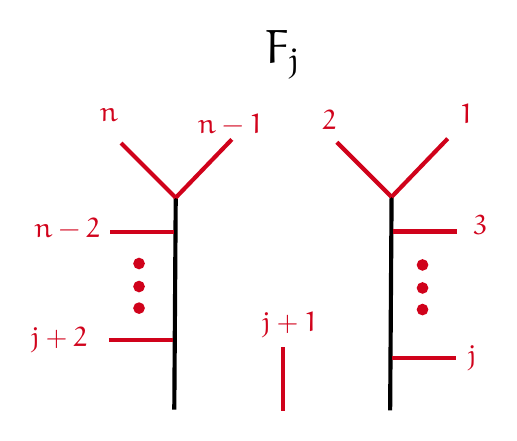
\begin{tikzpicture}[x=0.65pt,y=0.65pt,yscale=-1,xscale=1]
%uncomment if require: \path (0,269); %set diagram left start at 0, and has height of 269

%Straight Lines [id:da56945223255554] 
\draw [line width=1.5]    (109.53,225.47) -- (110.33,107.67) ;
%Straight Lines [id:da2259435687109952] 
\draw [line width=1.5]    (229.53,225.87) -- (230.33,107.27) ;
%Straight Lines [id:da3385812038286169] 
\draw [color={rgb, 255:red, 208; green, 2; blue, 27 }  ,draw opacity=1 ][line width=1.5]    (169.93,190.87) -- (169.93,226.07) ;
%Straight Lines [id:da1395794510635593] 
\draw [color={rgb, 255:red, 208; green, 2; blue, 27 }  ,draw opacity=1 ][line width=1.5]    (141.53,75.27) -- (110.33,107.67) ;
%Straight Lines [id:da858796201086198] 
\draw [color={rgb, 255:red, 208; green, 2; blue, 27 }  ,draw opacity=1 ][line width=1.5]    (261.53,74.87) -- (230.33,107.27) ;
%Straight Lines [id:da4853292127947866] 
\draw [color={rgb, 255:red, 208; green, 2; blue, 27 }  ,draw opacity=1 ][line width=1.5]    (79.93,77.27) -- (110.33,107.67) ;
%Straight Lines [id:da8547093259020446] 
\draw [color={rgb, 255:red, 208; green, 2; blue, 27 }  ,draw opacity=1 ][line width=1.5]    (199.93,76.87) -- (230.33,107.27) ;
%Straight Lines [id:da0859512914612981] 
\draw [color={rgb, 255:red, 208; green, 2; blue, 27 }  ,draw opacity=1 ][line width=1.5]    (73.93,126.87) -- (109.53,126.87) ;
%Straight Lines [id:da14272211877656216] 
\draw [color={rgb, 255:red, 208; green, 2; blue, 27 }  ,draw opacity=1 ][line width=1.5]    (73.13,186.87) -- (108.73,186.87) ;
%Straight Lines [id:da35725121665246573] 
\draw [color={rgb, 255:red, 208; green, 2; blue, 27 }  ,draw opacity=1 ][line width=1.5]    (231.13,126.47) -- (266.73,126.47) ;
%Straight Lines [id:da9110024677556066] 
\draw [color={rgb, 255:red, 208; green, 2; blue, 27 }  ,draw opacity=1 ][line width=1.5]    (230.33,196.87) -- (265.93,196.87) ;
%Shape: Circle [id:dp36396979514190675] 
\draw  [color={rgb, 255:red, 208; green, 2; blue, 27 }  ,draw opacity=1 ][fill={rgb, 255:red, 208; green, 2; blue, 27 }  ,fill opacity=1 ][line width=1.5]  (87.93,144.27) .. controls (87.93,143.16) and (88.83,142.27) .. (89.93,142.27) .. controls (91.04,142.27) and (91.93,143.16) .. (91.93,144.27) .. controls (91.93,145.37) and (91.04,146.27) .. (89.93,146.27) .. controls (88.83,146.27) and (87.93,145.37) .. (87.93,144.27) -- cycle ;
%Shape: Circle [id:dp3785400190350803] 
\draw  [color={rgb, 255:red, 208; green, 2; blue, 27 }  ,draw opacity=1 ][fill={rgb, 255:red, 208; green, 2; blue, 27 }  ,fill opacity=1 ][line width=1.5]  (87.93,157.07) .. controls (87.93,155.96) and (88.83,155.07) .. (89.93,155.07) .. controls (91.04,155.07) and (91.93,155.96) .. (91.93,157.07) .. controls (91.93,158.17) and (91.04,159.07) .. (89.93,159.07) .. controls (88.83,159.07) and (87.93,158.17) .. (87.93,157.07) -- cycle ;
%Shape: Circle [id:dp9513177640100214] 
\draw  [color={rgb, 255:red, 208; green, 2; blue, 27 }  ,draw opacity=1 ][fill={rgb, 255:red, 208; green, 2; blue, 27 }  ,fill opacity=1 ][line width=1.5]  (87.93,169.07) .. controls (87.93,167.96) and (88.83,167.07) .. (89.93,167.07) .. controls (91.04,167.07) and (91.93,167.96) .. (91.93,169.07) .. controls (91.93,170.17) and (91.04,171.07) .. (89.93,171.07) .. controls (88.83,171.07) and (87.93,170.17) .. (87.93,169.07) -- cycle ;
%Shape: Circle [id:dp30708084904995303] 
\draw  [color={rgb, 255:red, 208; green, 2; blue, 27 }  ,draw opacity=1 ][fill={rgb, 255:red, 208; green, 2; blue, 27 }  ,fill opacity=1 ][line width=1.5]  (245.53,145.07) .. controls (245.53,143.96) and (246.43,143.07) .. (247.53,143.07) .. controls (248.64,143.07) and (249.53,143.96) .. (249.53,145.07) .. controls (249.53,146.17) and (248.64,147.07) .. (247.53,147.07) .. controls (246.43,147.07) and (245.53,146.17) .. (245.53,145.07) -- cycle ;
%Shape: Circle [id:dp2197597647739662] 
\draw  [color={rgb, 255:red, 208; green, 2; blue, 27 }  ,draw opacity=1 ][fill={rgb, 255:red, 208; green, 2; blue, 27 }  ,fill opacity=1 ][line width=1.5]  (245.53,157.87) .. controls (245.53,156.76) and (246.43,155.87) .. (247.53,155.87) .. controls (248.64,155.87) and (249.53,156.76) .. (249.53,157.87) .. controls (249.53,158.97) and (248.64,159.87) .. (247.53,159.87) .. controls (246.43,159.87) and (245.53,158.97) .. (245.53,157.87) -- cycle ;
%Shape: Circle [id:dp5671918280089876] 
\draw  [color={rgb, 255:red, 208; green, 2; blue, 27 }  ,draw opacity=1 ][fill={rgb, 255:red, 208; green, 2; blue, 27 }  ,fill opacity=1 ][line width=1.5]  (245.53,169.87) .. controls (245.53,168.76) and (246.43,167.87) .. (247.53,167.87) .. controls (248.64,167.87) and (249.53,168.76) .. (249.53,169.87) .. controls (249.53,170.97) and (248.64,171.87) .. (247.53,171.87) .. controls (246.43,171.87) and (245.53,170.97) .. (245.53,169.87) -- cycle ;

% Text Node
\draw (158.33,13.47) node [anchor=north west][inner sep=0.75pt]  [font=\LARGE]  {$F_{j}$};
% Text Node
\draw (266.73,54.47) node [anchor=north west][inner sep=0.75pt]    {$\textcolor[rgb]{0.82,0.01,0.11}{1}$};
% Text Node
\draw (190.33,57.67) node [anchor=north west][inner sep=0.75pt]    {$\textcolor[rgb]{0.82,0.01,0.11}{2}$};
% Text Node
\draw (274.33,116.07) node [anchor=north west][inner sep=0.75pt]    {$\textcolor[rgb]{0.82,0.01,0.11}{3}$};
% Text Node
\draw (66.73,56.87) node [anchor=north west][inner sep=0.75pt]    {$\textcolor[rgb]{0.82,0.01,0.11}{n}$};
% Text Node
\draw (121.13,60.07) node [anchor=north west][inner sep=0.75pt]    {$\textcolor[rgb]{0.82,0.01,0.11}{n-1}$};
% Text Node
\draw (30.33,117.67) node [anchor=north west][inner sep=0.75pt]    {$\textcolor[rgb]{0.82,0.01,0.11}{n-2}$};
% Text Node
\draw (271.13,188.47) node [anchor=north west][inner sep=0.75pt]    {$\textcolor[rgb]{0.82,0.01,0.11}{j}$};
% Text Node
\draw (156.73,170.07) node [anchor=north west][inner sep=0.75pt]    {$\textcolor[rgb]{0.82,0.01,0.11}{j+1}$};
% Text Node
\draw (28.33,178.07) node [anchor=north west][inner sep=0.75pt]    {$\textcolor[rgb]{0.82,0.01,0.11}{j+2}$};


\end{tikzpicture}
    \caption{The marked fragment that attaches to the horizontal edge of $\tilde{T}$ to obtain the base graph $T$.}
    \label{fig:lpositivefragments}
\end{figure}
The number of marked fragments when $\ell>0$ is $n-2-2\ell=g+3+2\ell-2-2\ell=g-1$. There is a bijection between this solution set and the solution set constructed in \cite{troptev}. Since each cover counts with multiplicity equal to one, we have thus far shown that $\Tev_{g,\ell}^\trop\geq 2^g$ for positive $\ell$.

\subsection{Excluding further solutions} \label{sec:ellposexclude}
In this section, we exclude any further cover $\Gamma \to T$ from mapping to  the chosen point $p= (\overline{\Gamma},\overline{T})\in \Mgn{g,n}^\trop\times \Mgn{0,n}^\trop$. We follow similar arguments made in \cite{troptev}.

\subsubsection*{Fragments attaching to the active edge}
The same argument as in Section 4.3 in \cite{troptev} excludes all marked fragments besides those shown in Figure \ref{fig:markfrag}. We now exclude marked fragments $F_1$ and $F_{n-2}$. 

Recall that marked fragments $F_1$ and $F_{n-2}$ can only be placed on covers that have $i=0$, meaning that zero joined ends have to be added to complete the degree $d=g+1$ cover. When $\ell$ is positive, we must add $\ell$ joined ends to obtain a cover of degree $d+g+1+\ell$. Therefore, even when fragment $D$ is used zero times, $i>0$. Moreover, only the marked fragments shown in Figure \ref{fig:lpositivefragments} can be attached to covers.

\subsubsection*{Splitting of transpositions}
Recall that the genus part of the graph $\gGamma \to \gT $ contains at least $3g$ transpositions. 

\begin{claim}
    The marked tree part of the graph needs at least $g+2\ell$ transpositions.
\end{claim}
\begin{proof}
    There are $g+2\ell$ lengths $L_i$'s, each of which is much longer than the lengths on $\overline{\Gamma}$. Therefore, all marked points from $3$ to $n-2=g+1+2\ell$ must be stabilizing to the active path from an edge that it is the only mark on. There are at least $g+2\ell-1$ transpositions used to form such edges. Finally, in order to not have a relation between the lengths $x_{4g+2\ell}$ and $L_{g+2\ell}$, the branch that the marks $1$ and $2$ lie on must attach to an edge of degree at least $2$. In total, at least $g+2\ell$ transpositions are needed for the marked tree part of $\Gamma \to T$.
\end{proof}

The total number of transpositions is $4g+2\ell$, and therefore the number of transpositions on $\gGamma \to \gT$ is exactly $3g$ and the number on the marked tree part of $\Gamma \to T$ is $g+2\ell$.

Knowing that any new loop is added with exactly three transpositions we use the proof in Section 4.3 in \cite{troptev} to rule out all loop fragments besides $U$ and $D$. That proof also gives that all covers have a marked tree part that looks like some number of cuts followed by all joins and ending with the rest of the cuts. But then all possible solutions to our problem must be of the form of those we have exhibited, and there can be no more solutions and we have shown Theorem \ref{thm:ellpositive}.



%%%%%%%%%%%%%%%%%%%%%%%%%%%%%%%%%%%%%%%%%%%%%%%%%%%%%%%%%%%%%%%%%
\section{Tropical Tevelev degrees $\Tev^\trop_{g,\ell}$ for $\ell<0$}
\label{sec:ell<0}
When $\ell$ is negative, both the degree and the number of marked points become less than what they are in the $\ell=0$ case. Due to the degree being lower, we can not form the genus section of the covers in all of the same ways. For example, a genus part of the cover, $\gGamma \to \gT$, from the $\ell=0$ case used all of the degree to form the genus, that can not be made when the degree decreases. This leads to fewer ways to form the genus section. We can count the number of preimages using the same grid as used in the $\ell=0$ case but there are rows removed corresponding to the $\gGamma \to \gT$ from the $\ell=0$ case that are not possible. In this section, we go through examples in low genera when $\ell=-1$, then construct the number of solutions, and finally rule out any other possible solutions. 


\subsection{Examples in low genera and $\ell$ close to zero}
\subsubsection{$\ell=-1$:} 

Starting with $g=2$, in order to compute $\Tev_{2,-1}^\trop$, we must compute the degree of the map \[(\Fs\times\Ft):\Hur{2,2,3}^\trop \to \Mgn{2,3}^\trop \times \Mgn{0,3}^\trop.\]
Consider the point $p=(\overline{\Gamma},\overline{T})\in \Mgn{2,3}^\trop \times \Mgn{0,3}^\trop$ depicted in Figure \ref{fig:genim}. 

We start by constructing $\gGamma \to \gT$. The Riemann-Hurwitz formula states that there are 6 simple transpositions. There is one way to form a degree 2 cover that contains two disjoint loops. 

We then complete $\gGamma \to \gT$ to $\Gamma \to T$ by adding 3 marked points. Place marked point 3 at distance $y_5$ from the second loop, and place marked points 1 and 2 $y_6$ to the right on 3. There are no other ways to place the marked points so that $\Gamma \to T$ is a preimage of $p$. Therefore, we get one cover in $(\Fs\times \Ft)^{-1}(p)$ shown in Figure \ref{fig:l=-1,g=2}. We now compute the local degree of $(\Fs\times\Ft)$ at this inverse image. 

\begin{figure}[tb]
    \centering


\tikzset{every picture/.style={line width=0.75pt}} %set default line width to 0.75pt        

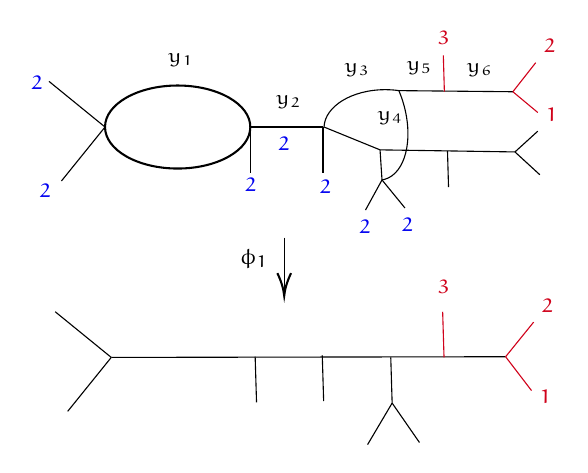
\begin{tikzpicture}[x=0.75pt,y=0.75pt,yscale=-1,xscale=1]
%uncomment if require: \path (0,253); %set diagram left start at 0, and has height of 253

%Straight Lines [id:da48667596104939514] 
\draw    (91,67) -- (64,45) ;
%Straight Lines [id:da06573015138186578] 
\draw    (91,67) -- (70,93) ;
%Shape: Ellipse [id:dp3309195306836237] 
\draw  [line width=0.75]  (91,67) .. controls (91,55.95) and (106.67,47) .. (126,47) .. controls (145.33,47) and (161,55.95) .. (161,67) .. controls (161,78.05) and (145.33,87) .. (126,87) .. controls (106.67,87) and (91,78.05) .. (91,67) -- cycle ;
%Straight Lines [id:da9807086882266265] 
\draw    (161,67) -- (196,67) ;
%Straight Lines [id:da6238727793368819] 
\draw    (161,67) -- (161,89) ;
%Straight Lines [id:da298455705850865] 
\draw    (196,67) -- (196,89) ;
%Shape: Arc [id:dp919092490919569] 
\draw  [draw opacity=0] (196.51,67) .. controls (196.93,57.01) and (209.97,49) .. (226,49) .. controls (228.26,49) and (230.45,49.16) .. (232.57,49.46) -- (226,67.5) -- cycle ; \draw   (196.51,67) .. controls (196.93,57.01) and (209.97,49) .. (226,49) .. controls (228.26,49) and (230.45,49.16) .. (232.57,49.46) ;  
%Shape: Arc [id:dp5081915109248467] 
\draw  [draw opacity=0] (232.57,49.46) .. controls (233.42,51.47) and (234.18,53.59) .. (234.82,55.8) .. controls (239.79,73.02) and (235.73,89.32) .. (225.75,92.2) .. controls (225.32,92.32) and (224.89,92.42) .. (224.45,92.49) -- (216.75,61.01) -- cycle ; \draw   (232.57,49.46) .. controls (233.42,51.47) and (234.18,53.59) .. (234.82,55.8) .. controls (239.79,73.02) and (235.73,89.32) .. (225.75,92.2) .. controls (225.32,92.32) and (224.89,92.42) .. (224.45,92.49) ;  
%Straight Lines [id:da9145252576600118] 
\draw    (196.51,67) -- (223.5,78) ;
%Straight Lines [id:da14428195925374432] 
\draw    (223.5,78) -- (224.45,92.49) ;
%Straight Lines [id:da5075490882587195] 
\draw    (224.45,92.49) -- (235.5,106) ;
%Straight Lines [id:da3381816466664722] 
\draw    (224.45,92.49) -- (216.5,107) ;
%Straight Lines [id:da8060692486381469] 
\draw    (223.5,78) -- (288.5,79) ;
%Straight Lines [id:da5710824833024439] 
\draw    (232.57,49.46) -- (287.5,50) ;
%Straight Lines [id:da58537954674785] 
\draw    (256,78.5) -- (256.5,96) ;
%Straight Lines [id:da9107013347313291] 
\draw [color={rgb, 255:red, 208; green, 2; blue, 27 }  ,draw opacity=1 ]   (254,32.5) -- (254.5,50) ;
%Straight Lines [id:da4036451488257369] 
\draw [color={rgb, 255:red, 208; green, 2; blue, 27 }  ,draw opacity=1 ]   (298.5,36) -- (287.5,50) ;
%Straight Lines [id:da3338490234401339] 
\draw [color={rgb, 255:red, 208; green, 2; blue, 27 }  ,draw opacity=1 ]   (287.5,50) -- (299.5,60) ;
%Straight Lines [id:da015223229627960189] 
\draw    (299.5,69) -- (288.5,79) ;
%Straight Lines [id:da8142170489624976] 
\draw    (288.5,79) -- (300.5,90) ;
%Straight Lines [id:da5285288231931149] 
\draw    (94,178) -- (67,156) ;
%Straight Lines [id:da30177727375004015] 
\draw    (94,178) -- (73,204) ;
%Straight Lines [id:da7642076060575798] 
\draw    (94,178) -- (284,177.67) ;
%Straight Lines [id:da46631276305260005] 
\draw    (163.33,177.67) -- (164,199.67) ;
%Straight Lines [id:da41815386703662316] 
\draw    (195.67,177) -- (196.33,199) ;
%Straight Lines [id:da23287655783069394] 
\draw    (177.33,120.33) -- (177.33,146.33) ;
\draw [shift={(177.33,148.33)}, rotate = 270] [color={rgb, 255:red, 0; green, 0; blue, 0 }  ][line width=0.75]    (10.93,-3.29) .. controls (6.95,-1.4) and (3.31,-0.3) .. (0,0) .. controls (3.31,0.3) and (6.95,1.4) .. (10.93,3.29)   ;
%Straight Lines [id:da6344693810700499] 
\draw    (228.67,178) -- (229.33,200) ;
%Straight Lines [id:da17423541038121093] 
\draw    (229.33,200) -- (217.5,220) ;
%Straight Lines [id:da8706927086665857] 
\draw    (229.33,200) -- (242.5,219) ;
%Straight Lines [id:da050828981852048205] 
\draw [color={rgb, 255:red, 208; green, 2; blue, 27 }  ,draw opacity=1 ]   (253.67,156) -- (254.33,178) ;
%Straight Lines [id:da9474313212108845] 
\draw [color={rgb, 255:red, 208; green, 2; blue, 27 }  ,draw opacity=1 ]   (297.5,161) -- (284,177.67) ;
%Straight Lines [id:da5428448657070848] 
\draw [color={rgb, 255:red, 208; green, 2; blue, 27 }  ,draw opacity=1 ]   (284,177.67) -- (296.5,194) ;

% Text Node
\draw (54,41.4) node [anchor=north west][inner sep=0.75pt]  [font=\scriptsize,color={rgb, 255:red, 1; green, 1; blue, 240 }  ,opacity=1 ]  {$2$};
% Text Node
\draw (58,93.4) node [anchor=north west][inner sep=0.75pt]  [font=\scriptsize,color={rgb, 255:red, 1; green, 1; blue, 240 }  ,opacity=1 ]  {$2$};
% Text Node
\draw (157,90.4) node [anchor=north west][inner sep=0.75pt]  [font=\scriptsize,color={rgb, 255:red, 1; green, 1; blue, 240 }  ,opacity=1 ]  {$2$};
% Text Node
\draw (193,91.4) node [anchor=north west][inner sep=0.75pt]  [font=\scriptsize,color={rgb, 255:red, 1; green, 1; blue, 240 }  ,opacity=1 ]  {$2$};
% Text Node
\draw (212,110.4) node [anchor=north west][inner sep=0.75pt]  [font=\scriptsize,color={rgb, 255:red, 1; green, 1; blue, 240 }  ,opacity=1 ]  {$2$};
% Text Node
\draw (232.5,109.4) node [anchor=north west][inner sep=0.75pt]  [font=\scriptsize,color={rgb, 255:red, 1; green, 1; blue, 240 }  ,opacity=1 ]  {$2$};
% Text Node
\draw (173,70.4) node [anchor=north west][inner sep=0.75pt]  [font=\scriptsize,color={rgb, 255:red, 1; green, 1; blue, 240 }  ,opacity=1 ]  {$2$};
% Text Node
\draw (250,19.4) node [anchor=north west][inner sep=0.75pt]  [font=\scriptsize,color={rgb, 255:red, 208; green, 2; blue, 27 }  ,opacity=1 ]  {$3$};
% Text Node
\draw (301,23.4) node [anchor=north west][inner sep=0.75pt]  [font=\scriptsize,color={rgb, 255:red, 208; green, 2; blue, 27 }  ,opacity=1 ]  {$2$};
% Text Node
\draw (302,56.4) node [anchor=north west][inner sep=0.75pt]  [font=\scriptsize,color={rgb, 255:red, 208; green, 2; blue, 27 }  ,opacity=1 ]  {$1$};
% Text Node
\draw (120,30.4) node [anchor=north west][inner sep=0.75pt]  [font=\scriptsize]  {$y_{1}$};
% Text Node
\draw (172,50.4) node [anchor=north west][inner sep=0.75pt]  [font=\scriptsize]  {$y_{2}$};
% Text Node
\draw (205,35.4) node [anchor=north west][inner sep=0.75pt]  [font=\scriptsize]  {$y_{3}$};
% Text Node
\draw (221,58.4) node [anchor=north west][inner sep=0.75pt]  [font=\scriptsize]  {$y_{4}$};
% Text Node
\draw (235,34.4) node [anchor=north west][inner sep=0.75pt]  [font=\scriptsize]  {$y_{5}$};
% Text Node
\draw (264,35.4) node [anchor=north west][inner sep=0.75pt]  [font=\scriptsize]  {$y_{6}$};
% Text Node
\draw (250,139.4) node [anchor=north west][inner sep=0.75pt]  [font=\scriptsize,color={rgb, 255:red, 208; green, 2; blue, 27 }  ,opacity=1 ]  {$3$};
% Text Node
\draw (300,148.4) node [anchor=north west][inner sep=0.75pt]  [font=\scriptsize,color={rgb, 255:red, 208; green, 2; blue, 27 }  ,opacity=1 ]  {$2$};
% Text Node
\draw (299,192.4) node [anchor=north west][inner sep=0.75pt]  [font=\scriptsize,color={rgb, 255:red, 208; green, 2; blue, 27 }  ,opacity=1 ]  {$1$};
% Text Node
\draw (155,124.4) node [anchor=north west][inner sep=0.75pt]  [font=\footnotesize]  {$\phi _{1}$};


\end{tikzpicture}
    \caption{The one cover in $(\Fs\times \Ft)^{-1}(p)$ for $\ell=-1$ and $g=2$.}
    \label{fig:l=-1,g=2}
\end{figure}

To calculate the local Hurwitz number, every vertex in $\Gamma_1$ is either trivalent with degree one edges in all directions or two edges of degree 2 in different directions and 2 edges of degree 1 in the same direction. Both of these types of vertices have local Hurwitz number equal to 1, therefore the product of all local Hurwitz numbers is 1. 

The cover has an automorphism factor of 2 corresponding to switching each pair of ends of branching type $2$ and their inverse images. Altogether, we have \begin{equation*}
    \frac{|\Aut(\overline{\Gamma_1})|}{|\Aut(\phi_1)|} = \frac{1}{4}.
\end{equation*}

To calculate the dilation factor, we set up the following matrix representing the $x_i$'s in terms of the $y_k$'s: 
\[M_1=\begin{blockarray}{ccccccc}
   &y_1 & y_2 & y_3 & y_4 & y_5 & y_6 \\
    \begin{block}{c[cccccc]}
      x_1 & 2 & 0 & 0 & 0 & 0 & 0\\
      x_2 & 0 & 1 & 0 & 0 & 0 & 0\\
      x_3 & 0 & 0 & 1 & 0 & 0 & 0\\
      x_4 & 0 & 0 & 1 & 2 & 0 & 0\\
      x_5 & 0 & 0 & 0 & 0 & 1 & 0\\
      x_6 & 0 & 0 & 0 & 0 & 0 & 1\\
    \end{block}
  \end{blockarray}
\]
We see that $|\det M_1 |=4$.
All together the multiplicity of each cover in $(\Fs\times\Ft)^{-1}(p)$ is $1\cdot \frac{1}{4}\cdot 4=1$. Since we have one inverse image with multiplicity one,  we obtain $\Tev^\trop_{2,-1} = 1$.

To interpret $\Tev^\trop_{2,-1}$ in another way, we compare the grid of solutions for $\ell = -1$ and $g=2$ with the grid of solutions for $\ell=0$ and $g=2$ shown in Figure \ref{fig:l=0g=2}. Although the marked point configurations and total degrees are different, we obtain organizations according to the same active edge degrees. When $\ell=-1$, we lose the top row of the grid corresponding to having an active edge of degree 3. The cover $\phi_{2,2} $ in Figure \ref{fig:l=0g=2} with the joined end removed and no marked points is the same as $\phi_1$ in Figure \ref{fig:l=-1,g=2} with no marked points as shown in Figure \ref{fig:removejoinedend}. 

\begin{figure}[tb]
    \centering


\tikzset{every picture/.style={line width=0.75pt}} %set default line width to 0.75pt        

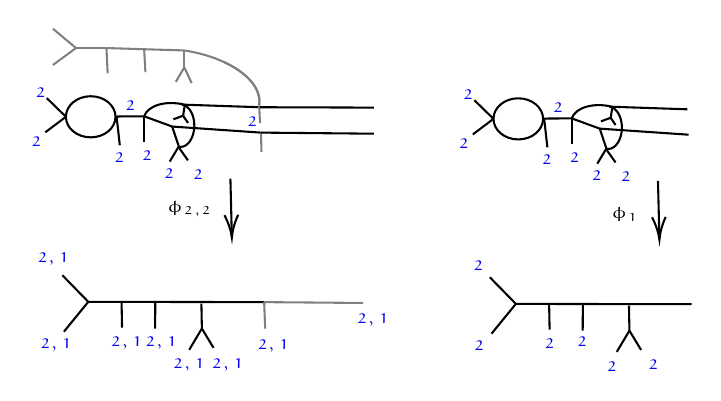
\begin{tikzpicture}[x=0.75pt,y=0.75pt,yscale=-1,xscale=1]
%uncomment if require: \path (0,215); %set diagram left start at 0, and has height of 215

%Straight Lines [id:da9563807978855503] 
\draw [line width=0.75]    (52.79,147.54) -- (137.53,147.69) ;
%Straight Lines [id:da5693673194460929] 
\draw [line width=0.75]    (40.28,134.73) -- (52.79,147.54) ;
%Straight Lines [id:da8024651596664985] 
\draw [line width=0.75]    (41.06,161.9) -- (52.79,147.54) ;
%Straight Lines [id:da7800629861272803] 
\draw [line width=0.75]    (69.05,159.96) -- (68.81,147.38) ;
%Straight Lines [id:da5204823687131332] 
\draw [line width=0.75]    (84.99,160.42) -- (85.07,147.69) ;
%Straight Lines [id:da772961360819471] 
\draw [line width=0.75]    (107.51,160.42) -- (107.28,148.39) ;
%Straight Lines [id:da024672535654581162] 
\draw [line width=0.75]    (107.51,160.42) -- (113.14,169.74) ;
%Straight Lines [id:da06857667222794617] 
\draw [line width=0.75]    (101.41,170.67) -- (107.51,160.42) ;
%Straight Lines [id:da8264865597199793] 
\draw [color={rgb, 255:red, 128; green, 128; blue, 128 }  ,draw opacity=1 ][line width=0.75]    (137.53,147.69) -- (138,160.42) ;
%Straight Lines [id:da10272477210475461] 
\draw [line width=0.75]    (66.42,58.25) -- (67.98,72.13) ;
%Straight Lines [id:da7821130761299231] 
\draw [line width=0.75]    (66.42,58.25) -- (79.71,58.16) ;
%Straight Lines [id:da8316806585604914] 
\draw [line width=0.75]    (79.71,58.16) -- (79.71,70.67) ;
%Shape: Arc [id:dp030108941436313152] 
\draw  [draw opacity=0][line width=0.75]  (79.71,58.15) .. controls (81.54,52.89) and (90.05,50.38) .. (99.22,52.55) .. controls (99.25,52.55) and (99.27,52.56) .. (99.3,52.57) -- (96.76,62.83) -- cycle ; \draw  [line width=0.75]  (79.71,58.15) .. controls (81.54,52.89) and (90.05,50.38) .. (99.22,52.55) .. controls (99.25,52.55) and (99.27,52.56) .. (99.3,52.57) ;  
%Straight Lines [id:da4584599314293232] 
\draw [line width=0.75]    (79.71,58.16) -- (93.2,63.1) ;
%Straight Lines [id:da2834171328698174] 
\draw [line width=0.75]    (93.2,63.1) -- (96.71,73.58) ;
%Shape: Arc [id:dp5103164610766322] 
\draw  [draw opacity=0][line width=0.75]  (97.88,52.54) .. controls (101.3,52.92) and (103.95,57.38) .. (103.88,62.8) .. controls (103.81,68.43) and (100.82,72.96) .. (97.2,72.92) .. controls (96.91,72.92) and (96.61,72.88) .. (96.33,72.82) -- (97.33,62.72) -- cycle ; \draw  [line width=0.75]  (97.88,52.54) .. controls (101.3,52.92) and (103.95,57.38) .. (103.88,62.8) .. controls (103.81,68.43) and (100.82,72.96) .. (97.2,72.92) .. controls (96.91,72.92) and (96.61,72.88) .. (96.33,72.82) ;  
%Straight Lines [id:da8503751846006515] 
\draw [line width=0.75]    (96.32,72.82) -- (92.02,79.99) ;
%Straight Lines [id:da9363528139125885] 
\draw [line width=0.75]    (96.71,73.58) -- (100.82,79.4) ;
%Straight Lines [id:da05467429569733895] 
\draw [line width=0.75]    (93.2,63.1) -- (136,66.02) ;
%Straight Lines [id:da11853253658710905] 
\draw [line width=0.75]    (99.3,52.57) -- (135.41,53.79) ;
%Straight Lines [id:da9760801690998557] 
\draw [color={rgb, 255:red, 128; green, 128; blue, 128 }  ,draw opacity=1 ][line width=0.75]    (46.88,25.27) -- (35.74,33.42) ;
%Straight Lines [id:da7628517322927273] 
\draw [color={rgb, 255:red, 128; green, 128; blue, 128 }  ,draw opacity=1 ][line width=0.75]    (35.74,15.96) -- (46.88,25.27) ;
%Straight Lines [id:da3229723461052896] 
\draw [color={rgb, 255:red, 128; green, 128; blue, 128 }  ,draw opacity=1 ][line width=0.75]    (46.88,25.27) -- (61.53,25.27) ;
%Straight Lines [id:da601117495459323] 
\draw [color={rgb, 255:red, 128; green, 128; blue, 128 }  ,draw opacity=1 ][line width=0.75]    (61.53,25.27) -- (62.12,37.49) ;
%Straight Lines [id:da15704403979346537] 
\draw [color={rgb, 255:red, 128; green, 128; blue, 128 }  ,draw opacity=1 ][line width=0.75]    (61.53,25.27) -- (79.71,25.85) ;
%Straight Lines [id:da2066563988080945] 
\draw [color={rgb, 255:red, 128; green, 128; blue, 128 }  ,draw opacity=1 ][line width=0.75]    (79.71,25.85) -- (80.3,36.91) ;
%Straight Lines [id:da8988903736731497] 
\draw [color={rgb, 255:red, 128; green, 128; blue, 128 }  ,draw opacity=1 ][line width=0.75]    (79.71,25.85) -- (99.06,26.43) ;
%Straight Lines [id:da021505217759042683] 
\draw [color={rgb, 255:red, 128; green, 128; blue, 128 }  ,draw opacity=1 ][line width=0.75]    (99.06,26.43) -- (99.06,34.58) ;
%Straight Lines [id:da8677594949149203] 
\draw [color={rgb, 255:red, 128; green, 128; blue, 128 }  ,draw opacity=1 ][line width=0.75]    (99.06,34.58) -- (102.58,42.15) ;
%Straight Lines [id:da9848311132403216] 
\draw [color={rgb, 255:red, 128; green, 128; blue, 128 }  ,draw opacity=1 ][line width=0.75]    (99.06,34.58) -- (94.96,41.57) ;
%Straight Lines [id:da8015998522990684] 
\draw [line width=0.75]    (99.3,52.57) -- (98.47,57.87) ;
%Straight Lines [id:da42899159946362553] 
\draw [line width=0.75]    (98.47,57.87) -- (93.78,59.61) ;
%Straight Lines [id:da1475304985126371] 
\draw [line width=0.75]    (98.47,57.87) -- (100.82,61.36) ;
%Shape: Arc [id:dp5684062063626101] 
\draw  [draw opacity=0][line width=0.75]  (99.04,26.43) .. controls (120.51,29.73) and (136.41,40.85) .. (135.19,52.21) .. controls (135.16,52.42) and (135.14,52.64) .. (135.1,52.86) -- (92.82,47.7) -- cycle ; \draw  [color={rgb, 255:red, 128; green, 128; blue, 128 }  ,draw opacity=1 ][line width=0.75]  (99.04,26.43) .. controls (120.51,29.73) and (136.41,40.85) .. (135.19,52.21) .. controls (135.16,52.42) and (135.14,52.64) .. (135.1,52.86) ;  
%Straight Lines [id:da1803594354638387] 
\draw [color={rgb, 255:red, 128; green, 128; blue, 128 }  ,draw opacity=1 ][line width=0.75]    (135.1,52.85) -- (135.53,61.42) ;
%Straight Lines [id:da24906176348625553] 
\draw [color={rgb, 255:red, 128; green, 128; blue, 128 }  ,draw opacity=1 ][line width=0.75]    (136,66.02) -- (136.23,75.33) ;
%Straight Lines [id:da22114040397385248] 
\draw [line width=0.75]    (135.41,53.79) -- (190.41,53.97) ;
%Straight Lines [id:da9718732831871011] 
\draw [line width=0.75]    (136,66.02) -- (190.41,66.54) ;
%Straight Lines [id:da47390891447306105] 
\draw [line width=0.75]    (121.26,88.23) -- (121.91,114.64) ;
\draw [shift={(121.96,116.64)}, rotate = 268.58] [color={rgb, 255:red, 0; green, 0; blue, 0 }  ][line width=0.75]    (10.93,-3.29) .. controls (6.95,-1.4) and (3.31,-0.3) .. (0,0) .. controls (3.31,0.3) and (6.95,1.4) .. (10.93,3.29)   ;
%Straight Lines [id:da6016144096401204] 
\draw [line width=0.75]    (32.81,49.42) -- (42.01,58.39) ;
%Straight Lines [id:da5422696366497455] 
\draw [line width=0.75]    (42.01,58.39) -- (32.08,65.87) ;
%Shape: Ellipse [id:dp11844052076558587] 
\draw  [line width=0.75]  (42.01,58.39) .. controls (42.01,52.92) and (47.35,48.49) .. (53.95,48.49) .. controls (60.55,48.49) and (65.9,52.92) .. (65.9,58.39) .. controls (65.9,63.87) and (60.55,68.3) .. (53.95,68.3) .. controls (47.35,68.3) and (42.01,63.87) .. (42.01,58.39) -- cycle ;
%Shape: Arc [id:dp5825993959152749] 
\draw  [draw opacity=0][line width=0.75]  (117.97,31.92) .. controls (129.11,37.03) and (136.02,44.56) .. (135.19,52.19) .. controls (135.17,52.41) and (135.14,52.62) .. (135.1,52.84) -- (92.82,47.68) -- cycle ; \draw  [color={rgb, 255:red, 128; green, 128; blue, 128 }  ,draw opacity=1 ][line width=0.75]  (117.97,31.92) .. controls (129.11,37.03) and (136.02,44.56) .. (135.19,52.19) .. controls (135.17,52.41) and (135.14,52.62) .. (135.1,52.84) ;  
%Straight Lines [id:da5278742128678828] 
\draw [color={rgb, 255:red, 128; green, 128; blue, 128 }  ,draw opacity=1 ][line width=0.75]    (137.53,147.69) -- (185.25,148.09) ;
%Straight Lines [id:da7561985382710854] 
\draw [line width=0.75]    (258.79,148.54) -- (343.53,148.69) ;
%Straight Lines [id:da4407714516845751] 
\draw [line width=0.75]    (246.28,135.73) -- (258.79,148.54) ;
%Straight Lines [id:da09224410674738759] 
\draw [line width=0.75]    (247.06,162.9) -- (258.79,148.54) ;
%Straight Lines [id:da9617199383071555] 
\draw [line width=0.75]    (275.05,160.96) -- (274.81,148.38) ;
%Straight Lines [id:da41762394238162104] 
\draw [line width=0.75]    (290.99,161.42) -- (291.07,148.69) ;
%Straight Lines [id:da44094585451919666] 
\draw [line width=0.75]    (313.51,161.42) -- (313.28,149.39) ;
%Straight Lines [id:da10550427485382707] 
\draw [line width=0.75]    (313.51,161.42) -- (319.14,170.74) ;
%Straight Lines [id:da709432824745488] 
\draw [line width=0.75]    (307.41,171.67) -- (313.51,161.42) ;
%Straight Lines [id:da507598091988962] 
\draw [line width=0.75]    (272.42,59.25) -- (273.98,73.13) ;
%Straight Lines [id:da0014591065983413642] 
\draw [line width=0.75]    (272.42,59.25) -- (285.71,59.16) ;
%Straight Lines [id:da20963426866497636] 
\draw [line width=0.75]    (285.71,59.16) -- (285.71,71.67) ;
%Shape: Arc [id:dp5261911988516577] 
\draw  [draw opacity=0][line width=0.75]  (285.71,59.15) .. controls (287.54,53.89) and (296.05,51.38) .. (305.22,53.55) .. controls (305.25,53.55) and (305.27,53.56) .. (305.3,53.57) -- (302.76,63.83) -- cycle ; \draw  [line width=0.75]  (285.71,59.15) .. controls (287.54,53.89) and (296.05,51.38) .. (305.22,53.55) .. controls (305.25,53.55) and (305.27,53.56) .. (305.3,53.57) ;  
%Straight Lines [id:da8260574789714594] 
\draw [line width=0.75]    (285.71,59.16) -- (299.2,64.1) ;
%Straight Lines [id:da43401792405177986] 
\draw [line width=0.75]    (299.2,64.1) -- (302.71,74.58) ;
%Shape: Arc [id:dp8823492962450681] 
\draw  [draw opacity=0][line width=0.75]  (303.88,53.54) .. controls (307.3,53.92) and (309.95,58.38) .. (309.88,63.8) .. controls (309.81,69.43) and (306.82,73.96) .. (303.2,73.92) .. controls (302.91,73.92) and (302.61,73.88) .. (302.33,73.82) -- (303.33,63.72) -- cycle ; \draw  [line width=0.75]  (303.88,53.54) .. controls (307.3,53.92) and (309.95,58.38) .. (309.88,63.8) .. controls (309.81,69.43) and (306.82,73.96) .. (303.2,73.92) .. controls (302.91,73.92) and (302.61,73.88) .. (302.33,73.82) ;  
%Straight Lines [id:da9161395302256867] 
\draw [line width=0.75]    (302.32,73.82) -- (298.02,80.99) ;
%Straight Lines [id:da0984385099054339] 
\draw [line width=0.75]    (302.71,74.58) -- (306.82,80.4) ;
%Straight Lines [id:da5885169976721725] 
\draw [line width=0.75]    (299.2,64.1) -- (342,67.02) ;
%Straight Lines [id:da08562822381228008] 
\draw [line width=0.75]    (305.3,53.57) -- (341.41,54.79) ;
%Straight Lines [id:da007596533846555564] 
\draw [line width=0.75]    (305.3,53.57) -- (304.47,58.87) ;
%Straight Lines [id:da754250846883223] 
\draw [line width=0.75]    (304.47,58.87) -- (299.78,60.61) ;
%Straight Lines [id:da9228848426810414] 
\draw [line width=0.75]    (304.47,58.87) -- (306.82,62.36) ;
%Straight Lines [id:da5894779722418189] 
\draw [line width=0.75]    (327.26,89.23) -- (327.91,115.64) ;
\draw [shift={(327.96,117.64)}, rotate = 268.58] [color={rgb, 255:red, 0; green, 0; blue, 0 }  ][line width=0.75]    (10.93,-3.29) .. controls (6.95,-1.4) and (3.31,-0.3) .. (0,0) .. controls (3.31,0.3) and (6.95,1.4) .. (10.93,3.29)   ;
%Straight Lines [id:da26272982402974243] 
\draw [line width=0.75]    (238.81,50.42) -- (248.01,59.39) ;
%Straight Lines [id:da6272965023466555] 
\draw [line width=0.75]    (248.01,59.39) -- (238.08,66.87) ;
%Shape: Ellipse [id:dp317098224058862] 
\draw  [line width=0.75]  (248.01,59.39) .. controls (248.01,53.92) and (253.35,49.49) .. (259.95,49.49) .. controls (266.55,49.49) and (271.9,53.92) .. (271.9,59.39) .. controls (271.9,64.87) and (266.55,69.3) .. (259.95,69.3) .. controls (253.35,69.3) and (248.01,64.87) .. (248.01,59.39) -- cycle ;

% Text Node
\draw (89.19,97.64) node [anchor=north west][inner sep=0.75pt]  [font=\fontsize{0.59em}{0.71em}\selectfont]  {$\phi _{2}{}_{,}{}_{2}$};
% Text Node
\draw (25.85,43.32) node [anchor=north west][inner sep=0.75pt]  [font=\tiny,color={rgb, 255:red, 1; green, 1; blue, 240 }  ,opacity=1 ]  {$2$};
% Text Node
\draw (23.85,66.65) node [anchor=north west][inner sep=0.75pt]  [font=\tiny,color={rgb, 255:red, 1; green, 1; blue, 240 }  ,opacity=1 ]  {$2$};
% Text Node
\draw (69.18,49.32) node [anchor=north west][inner sep=0.75pt]  [font=\tiny,color={rgb, 255:red, 1; green, 1; blue, 240 }  ,opacity=1 ]  {$2$};
% Text Node
\draw (77.18,73.32) node [anchor=north west][inner sep=0.75pt]  [font=\tiny,color={rgb, 255:red, 1; green, 1; blue, 240 }  ,opacity=1 ]  {$2$};
% Text Node
\draw (63.85,74.65) node [anchor=north west][inner sep=0.75pt]  [font=\tiny,color={rgb, 255:red, 1; green, 1; blue, 240 }  ,opacity=1 ]  {$2$};
% Text Node
\draw (87.85,81.99) node [anchor=north west][inner sep=0.75pt]  [font=\tiny,color={rgb, 255:red, 1; green, 1; blue, 240 }  ,opacity=1 ]  {$2$};
% Text Node
\draw (101.82,82.8) node [anchor=north west][inner sep=0.75pt]  [font=\tiny,color={rgb, 255:red, 1; green, 1; blue, 240 }  ,opacity=1 ]  {$2$};
% Text Node
\draw (127.91,57.19) node [anchor=north west][inner sep=0.75pt]  [font=\tiny,color={rgb, 255:red, 1; green, 1; blue, 240 }  ,opacity=1 ]  {$2$};
% Text Node
\draw (26.82,122.65) node [anchor=north west][inner sep=0.75pt]  [font=\tiny,color={rgb, 255:red, 1; green, 1; blue, 240 }  ,opacity=1 ]  {$2,1$};
% Text Node
\draw (28.15,163.99) node [anchor=north west][inner sep=0.75pt]  [font=\tiny,color={rgb, 255:red, 1; green, 1; blue, 240 }  ,opacity=1 ]  {$2,1$};
% Text Node
\draw (62.15,163.32) node [anchor=north west][inner sep=0.75pt]  [font=\tiny,color={rgb, 255:red, 1; green, 1; blue, 240 }  ,opacity=1 ]  {$2,1$};
% Text Node
\draw (78.82,163.32) node [anchor=north west][inner sep=0.75pt]  [font=\tiny,color={rgb, 255:red, 1; green, 1; blue, 240 }  ,opacity=1 ]  {$2,1$};
% Text Node
\draw (92.15,173.99) node [anchor=north west][inner sep=0.75pt]  [font=\tiny,color={rgb, 255:red, 1; green, 1; blue, 240 }  ,opacity=1 ]  {$2,1$};
% Text Node
\draw (110.82,173.99) node [anchor=north west][inner sep=0.75pt]  [font=\tiny,color={rgb, 255:red, 1; green, 1; blue, 240 }  ,opacity=1 ]  {$2,1$};
% Text Node
\draw (132.82,164.65) node [anchor=north west][inner sep=0.75pt]  [font=\tiny,color={rgb, 255:red, 1; green, 1; blue, 240 }  ,opacity=1 ]  {$2,1$};
% Text Node
\draw (180.82,151.99) node [anchor=north west][inner sep=0.75pt]  [font=\tiny,color={rgb, 255:red, 1; green, 1; blue, 240 }  ,opacity=1 ]  {$2,1$};
% Text Node
\draw (303.19,100.64) node [anchor=north west][inner sep=0.75pt]  [font=\fontsize{0.59em}{0.71em}\selectfont]  {$\phi _{1}$};
% Text Node
\draw (231.85,44.32) node [anchor=north west][inner sep=0.75pt]  [font=\tiny,color={rgb, 255:red, 1; green, 1; blue, 240 }  ,opacity=1 ]  {$2$};
% Text Node
\draw (229.85,67.65) node [anchor=north west][inner sep=0.75pt]  [font=\tiny,color={rgb, 255:red, 1; green, 1; blue, 240 }  ,opacity=1 ]  {$2$};
% Text Node
\draw (275.18,50.32) node [anchor=north west][inner sep=0.75pt]  [font=\tiny,color={rgb, 255:red, 1; green, 1; blue, 240 }  ,opacity=1 ]  {$2$};
% Text Node
\draw (283.18,74.32) node [anchor=north west][inner sep=0.75pt]  [font=\tiny,color={rgb, 255:red, 1; green, 1; blue, 240 }  ,opacity=1 ]  {$2$};
% Text Node
\draw (269.85,75.65) node [anchor=north west][inner sep=0.75pt]  [font=\tiny,color={rgb, 255:red, 1; green, 1; blue, 240 }  ,opacity=1 ]  {$2$};
% Text Node
\draw (293.85,82.99) node [anchor=north west][inner sep=0.75pt]  [font=\tiny,color={rgb, 255:red, 1; green, 1; blue, 240 }  ,opacity=1 ]  {$2$};
% Text Node
\draw (307.82,83.8) node [anchor=north west][inner sep=0.75pt]  [font=\tiny,color={rgb, 255:red, 1; green, 1; blue, 240 }  ,opacity=1 ]  {$2$};
% Text Node
\draw (236.82,126.65) node [anchor=north west][inner sep=0.75pt]  [font=\tiny,color={rgb, 255:red, 1; green, 1; blue, 240 }  ,opacity=1 ]  {$2$};
% Text Node
\draw (237.15,164.99) node [anchor=north west][inner sep=0.75pt]  [font=\tiny,color={rgb, 255:red, 1; green, 1; blue, 240 }  ,opacity=1 ]  {$2$};
% Text Node
\draw (271.15,164.32) node [anchor=north west][inner sep=0.75pt]  [font=\tiny,color={rgb, 255:red, 1; green, 1; blue, 240 }  ,opacity=1 ]  {$2$};
% Text Node
\draw (286.82,163.32) node [anchor=north west][inner sep=0.75pt]  [font=\tiny,color={rgb, 255:red, 1; green, 1; blue, 240 }  ,opacity=1 ]  {$2$};
% Text Node
\draw (301.15,174.99) node [anchor=north west][inner sep=0.75pt]  [font=\tiny,color={rgb, 255:red, 1; green, 1; blue, 240 }  ,opacity=1 ]  {$2$};
% Text Node
\draw (321.14,174.14) node [anchor=north west][inner sep=0.75pt]  [font=\tiny,color={rgb, 255:red, 1; green, 1; blue, 240 }  ,opacity=1 ]  {$2$};


\end{tikzpicture}
    \caption{The cover $\phi_{2,2} $ with the joined end removed and no marked points is the same as $\phi_1$ with no marked points.}
    \label{fig:removejoinedend}
\end{figure}

Moving to genus 3, to compute $\Tev_{3,-1}^\trop$, we must compute the degree of the map \[(\Fs\times\Ft):\Hur{3,3,4}^\trop \to \Mgn{3,4}^\trop \times \Mgn{0,4}^\trop.\]

\begin{figure}[tb]
    \centering
    \inputTikZ{\textwidth}{Figures/l=-1genuspaths}
    \caption{A graph showing for genus $g$ which degrees are possible for the active edge by adding $U$ and $D$. For $\ell=-1$, paths ending at vertices along the diagonal are not possible because $d=g$.}
    \label{fig:l=-1genuspaths}
\end{figure}
We start by constructing $\gGamma \to \gT$. Looking at Figure \ref{fig:l=-1genuspaths}, for $g=3$, there are 3 possible paths, but one of those paths ends at a vertex with active edge degree 4. Since $\ell=-1$, the degree of the cover is $3$, therefore, paths to that vertex are not possible. We conclude that there are two possible ways to construct $\gGamma \to \gT$, one by adding $U$ then $D$ and one by doing the opposite. Recall $U$ and $D$ are introduced in Figure \ref{fig:2genusoptions}. Note, both of these options have an active edge of degree 2. 

To complete the cover, we add $4$ marked points. The task of adding $4$ marked points to an active edge of degree 2 was done in detail in \cite{troptev}, there are 2 ways of doing so. Putting together the ways to form $\gGamma \to \gT$ with the ways to add marked points, we have $4$ total covers in the preimage of $p$, giving that $\Tev_{3,-1}^\trop=4$. Comparing the genus 3 grid of solutions when $\ell=-1$ in Figure \ref{fig:l=-1,g=3} to the grid of solutions when $\ell=0$ shown in Figure \ref{fig:g=3grid}, notice that the prior is missing the top row of solutions. 

\begin{figure}[tb]
    \centering


\tikzset{every picture/.style={line width=0.75pt}} %set default line width to 0.75pt        

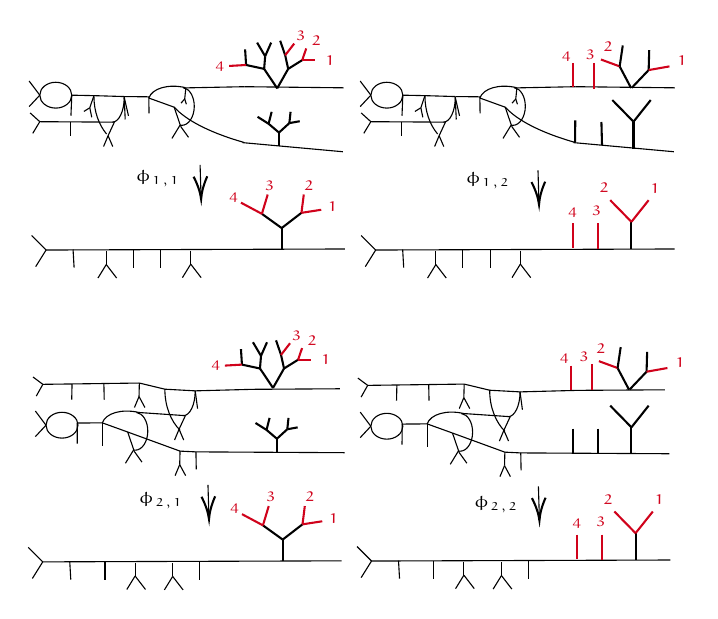
\begin{tikzpicture}[x=0.75pt,y=0.75pt,yscale=-1,xscale=1]
%uncomment if require: \path (0,297); %set diagram left start at 0, and has height of 297

%Straight Lines [id:da7501953254678526] 
\draw    (22.24,31.13) -- (27.37,37.95) ;
%Straight Lines [id:da10999901204899376] 
\draw    (27.37,37.95) -- (22.24,43.45) ;
%Shape: Ellipse [id:dp5376438300722879] 
\draw   (27.37,37.95) .. controls (27.37,34.51) and (30.82,31.73) .. (35.08,31.73) .. controls (39.33,31.73) and (42.78,34.51) .. (42.78,37.95) .. controls (42.78,41.38) and (39.33,44.17) .. (35.08,44.17) .. controls (30.82,44.17) and (27.37,41.38) .. (27.37,37.95) -- cycle ;
%Straight Lines [id:da08341687955798971] 
\draw    (42.78,37.95) -- (42.38,47.85) ;
%Straight Lines [id:da6014640354552216] 
\draw    (42.78,37.95) -- (53.44,38.17) ;
%Straight Lines [id:da6418994855785283] 
\draw    (27.37,50.72) -- (63.31,50.94) ;
%Shape: Arc [id:dp5585406661676995] 
\draw  [draw opacity=0] (59.54,56.66) .. controls (55.8,52.23) and (53.44,45.67) .. (53.44,38.35) .. controls (53.44,38.3) and (53.44,38.24) .. (53.44,38.19) -- (71.01,38.35) -- cycle ; \draw   (59.54,56.66) .. controls (55.8,52.23) and (53.44,45.67) .. (53.44,38.35) .. controls (53.44,38.3) and (53.44,38.24) .. (53.44,38.19) ;  
%Straight Lines [id:da26580076601489533] 
\draw    (63.31,50.94) -- (60.27,57.47) ;
%Straight Lines [id:da41665096598222506] 
\draw    (60.27,57.47) -- (62.52,62.69) ;
%Straight Lines [id:da24492860588649235] 
\draw    (60.27,57.47) -- (58.1,62.69) ;
%Straight Lines [id:da3137789984648365] 
\draw    (53.44,38.17) -- (68.05,38.61) ;
%Shape: Arc [id:dp7141535096789295] 
\draw  [draw opacity=0] (68.05,38.99) .. controls (68.05,39.02) and (68.05,39.04) .. (68.05,39.07) .. controls (68.05,45.62) and (65.5,50.94) .. (62.36,50.94) .. controls (62.34,50.94) and (62.31,50.94) .. (62.29,50.94) -- (62.36,39.07) -- cycle ; \draw   (68.05,38.99) .. controls (68.05,39.02) and (68.05,39.04) .. (68.05,39.07) .. controls (68.05,45.62) and (65.5,50.94) .. (62.36,50.94) .. controls (62.34,50.94) and (62.31,50.94) .. (62.29,50.94) ;  
%Straight Lines [id:da758574622073074] 
\draw    (41.99,50.72) -- (41.99,57.76) ;
%Straight Lines [id:da7421041471416328] 
\draw    (27.37,50.72) -- (22.71,46.49) ;
%Straight Lines [id:da15561203129489165] 
\draw    (27.37,50.72) -- (23.98,56.35) ;
%Straight Lines [id:da8087718175759058] 
\draw    (68.05,38.98) -- (70.1,47.9) ;
%Straight Lines [id:da9756459077434674] 
\draw    (68.05,38.61) -- (79.9,38.74) ;
%Straight Lines [id:da47035025742753445] 
\draw    (53.44,38.17) -- (51.46,44.02) ;
%Straight Lines [id:da3086342336050494] 
\draw    (51.46,44.02) -- (52.41,48.6) ;
%Straight Lines [id:da3991600653484533] 
\draw    (51.46,44.02) -- (48.62,45.79) ;
%Straight Lines [id:da13975537331665344] 
\draw    (68.05,38.98) -- (68.52,49.66) ;
%Straight Lines [id:da13033774543732068] 
\draw    (79.9,38.74) -- (80,46.7) ;
%Shape: Arc [id:dp9870053075144003] 
\draw  [draw opacity=0] (79.89,39.31) .. controls (81.55,34.62) and (89.27,32.39) .. (97.57,34.32) .. controls (97.6,34.33) and (97.62,34.33) .. (97.65,34.34) -- (95.34,43.49) -- cycle ; \draw   (79.89,39.31) .. controls (81.55,34.62) and (89.27,32.39) .. (97.57,34.32) .. controls (97.6,34.33) and (97.62,34.33) .. (97.65,34.34) ;  
%Straight Lines [id:da4321164728297624] 
\draw    (79.89,39.32) -- (92.11,43.73) ;
%Straight Lines [id:da682439713053733] 
\draw    (92.11,43.73) -- (95.3,53.07) ;
%Shape: Arc [id:dp08945057857848249] 
\draw  [draw opacity=0] (96.35,34.31) .. controls (99.45,34.65) and (101.86,38.63) .. (101.8,43.46) .. controls (101.73,48.48) and (99.02,52.52) .. (95.75,52.48) .. controls (95.48,52.48) and (95.22,52.45) .. (94.97,52.4) -- (95.86,43.39) -- cycle ; \draw   (96.35,34.31) .. controls (99.45,34.65) and (101.86,38.63) .. (101.8,43.46) .. controls (101.73,48.48) and (99.02,52.52) .. (95.75,52.48) .. controls (95.48,52.48) and (95.22,52.45) .. (94.97,52.4) ;  
%Straight Lines [id:da17987747041896407] 
\draw    (94.95,52.39) -- (91.05,58.78) ;
%Straight Lines [id:da6577571111421452] 
\draw    (95.3,53.07) -- (99.02,58.26) ;
%Straight Lines [id:da13323965476464616] 
\draw    (97.74,34.43) -- (97.19,39.77) ;
%Straight Lines [id:da3143879582764506] 
\draw    (97.19,39.77) -- (95.4,41.79) ;
%Straight Lines [id:da7051871749123992] 
\draw    (97.19,39.77) -- (97.99,42.33) ;

%Straight Lines [id:da46469254844190955] 
\draw    (97.74,34.43) -- (125.98,33.86) ;
%Straight Lines [id:da9456082956824281] 
\draw    (125.98,33.86) -- (173.8,34.4) ;
%Straight Lines [id:da008312361639953414] 
\draw    (125,60.8) -- (173.4,65.2) ;
%Straight Lines [id:da8399585405556644] 
\draw    (30.4,112.55) -- (174.4,112.05) ;
%Straight Lines [id:da09962794457980895] 
\draw    (30.4,112.55) -- (23.4,105.55) ;
%Straight Lines [id:da8607307760358878] 
\draw    (30.4,112.55) -- (25.4,120.55) ;
%Straight Lines [id:da9301557744752182] 
\draw    (43.4,112.3) -- (43.9,121.05) ;
%Straight Lines [id:da8497667218548253] 
\draw    (59.4,113.05) -- (59.4,119.55) ;
%Straight Lines [id:da7328940089975431] 
\draw    (59.4,119.55) -- (55.4,126.05) ;
%Straight Lines [id:da05865114046773945] 
\draw    (59.4,119.55) -- (64.4,126.05) ;
%Straight Lines [id:da6162134601568414] 
\draw    (72.4,112.3) -- (72.4,121.05) ;
%Straight Lines [id:da3753524957368779] 
\draw    (100.1,112.85) -- (100.1,119.35) ;
%Straight Lines [id:da6755831619453394] 
\draw    (100.1,119.35) -- (96.1,125.85) ;
%Straight Lines [id:da1995838880313192] 
\draw    (100.1,119.35) -- (105.1,125.85) ;
%Straight Lines [id:da9584224721175647] 
\draw    (85.6,112.3) -- (85.6,121.05) ;
%Straight Lines [id:da3268685967082292] 
\draw    (104.6,71.55) -- (105.04,86.05) ;
\draw [shift={(105.1,88.05)}, rotate = 268.26] [color={rgb, 255:red, 0; green, 0; blue, 0 }  ][line width=0.75]    (10.93,-3.29) .. controls (6.95,-1.4) and (3.31,-0.3) .. (0,0) .. controls (3.31,0.3) and (6.95,1.4) .. (10.93,3.29)   ;
%Straight Lines [id:da8206495219511116] 
\draw    (189.2,112.55) -- (333.2,112.05) ;
%Straight Lines [id:da6021689096668039] 
\draw    (189.2,112.55) -- (182.2,105.55) ;
%Straight Lines [id:da3095277580664062] 
\draw    (189.2,112.55) -- (184.2,120.55) ;
%Straight Lines [id:da31618505991969137] 
\draw    (202.2,112.3) -- (202.7,121.05) ;
%Straight Lines [id:da4448497808427032] 
\draw    (218.2,113.05) -- (218.2,119.55) ;
%Straight Lines [id:da02712895343177757] 
\draw    (218.2,119.55) -- (214.2,126.05) ;
%Straight Lines [id:da9297145125778894] 
\draw    (218.2,119.55) -- (223.2,126.05) ;
%Straight Lines [id:da49697906886712007] 
\draw    (231.2,112.3) -- (231.2,121.05) ;
%Straight Lines [id:da40351545366730646] 
\draw    (258.9,112.85) -- (258.9,119.35) ;
%Straight Lines [id:da4930148600851123] 
\draw    (258.9,119.35) -- (254.9,125.85) ;
%Straight Lines [id:da6580640902031893] 
\draw    (258.9,119.35) -- (263.9,125.85) ;
%Straight Lines [id:da3102666852884366] 
\draw    (244.4,112.3) -- (244.4,121.05) ;
%Straight Lines [id:da17934397660408696] 
\draw    (267.4,74.15) -- (267.84,88.65) ;
\draw [shift={(267.9,90.65)}, rotate = 268.26] [color={rgb, 255:red, 0; green, 0; blue, 0 }  ][line width=0.75]    (10.93,-3.29) .. controls (6.95,-1.4) and (3.31,-0.3) .. (0,0) .. controls (3.31,0.3) and (6.95,1.4) .. (10.93,3.29)   ;
%Straight Lines [id:da21205427473540817] 
\draw    (45.44,195.91) -- (45.4,205.8) ;
%Straight Lines [id:da32740906274072534] 
\draw    (45.44,195.91) -- (57.49,195.82) ;
%Straight Lines [id:da15084818146336376] 
\draw    (57.49,195.82) -- (57.49,206.98) ;
%Shape: Arc [id:dp3355825099359817] 
\draw  [draw opacity=0] (57.49,195.82) .. controls (59.15,191.13) and (66.86,188.9) .. (75.17,190.83) .. controls (75.19,190.84) and (75.22,190.84) .. (75.24,190.85) -- (72.94,200) -- cycle ; \draw   (57.49,195.82) .. controls (59.15,191.13) and (66.86,188.9) .. (75.17,190.83) .. controls (75.19,190.84) and (75.22,190.84) .. (75.24,190.85) ;  
%Straight Lines [id:da32540564451459364] 
\draw    (57.49,195.82) -- (69.71,200.23) ;
%Straight Lines [id:da9841588579297875] 
\draw    (69.71,200.23) -- (72.9,209.57) ;
%Shape: Arc [id:dp747103583064751] 
\draw  [draw opacity=0] (73.95,190.81) .. controls (77.05,191.15) and (79.46,195.13) .. (79.4,199.96) .. controls (79.33,204.98) and (76.62,209.02) .. (73.35,208.98) .. controls (73.08,208.98) and (72.82,208.95) .. (72.57,208.9) -- (73.46,199.89) -- cycle ; \draw   (73.95,190.81) .. controls (77.05,191.15) and (79.46,195.13) .. (79.4,199.96) .. controls (79.33,204.98) and (76.62,209.02) .. (73.35,208.98) .. controls (73.08,208.98) and (72.82,208.95) .. (72.57,208.9) ;  
%Straight Lines [id:da37315775230784576] 
\draw    (72.55,208.89) -- (68.65,215.28) ;
%Straight Lines [id:da49298591862550234] 
\draw    (72.9,209.57) -- (76.62,214.76) ;
%Straight Lines [id:da020228045349863777] 
\draw    (25.24,190.13) -- (30.37,196.95) ;
%Straight Lines [id:da9032504093532889] 
\draw    (30.37,196.95) -- (25.24,202.45) ;
%Shape: Ellipse [id:dp18554017572250703] 
\draw   (30.37,196.95) .. controls (30.37,193.51) and (33.82,190.73) .. (38.08,190.73) .. controls (42.33,190.73) and (45.78,193.51) .. (45.78,196.95) .. controls (45.78,200.38) and (42.33,203.17) .. (38.08,203.17) .. controls (33.82,203.17) and (30.37,200.38) .. (30.37,196.95) -- cycle ;
%Straight Lines [id:da09952566830545462] 
\draw    (28.85,177.26) -- (75.34,176.64) ;
%Straight Lines [id:da3958084971357294] 
\draw    (28.85,177.26) -- (24.11,173.74) ;
%Straight Lines [id:da7938097375992212] 
\draw    (28.85,177.26) -- (25.69,182.9) ;
%Straight Lines [id:da8988471368759743] 
\draw    (42.91,177.13) -- (42.75,184.66) ;
%Straight Lines [id:da15203369212120244] 
\draw    (75.34,176.64) -- (75.18,183.15) ;
%Straight Lines [id:da11699710647112682] 
\draw    (75.18,183.15) -- (78.03,188.43) ;
%Straight Lines [id:da6688442901383311] 
\draw    (75.18,183.15) -- (72.97,188.43) ;
%Straight Lines [id:da818704772442495] 
\draw    (58.25,177.08) -- (58.41,184.66) ;
%Shape: Arc [id:dp00476588558793356] 
\draw  [draw opacity=0] (94.96,199.39) .. controls (90.53,195) and (87.64,187.85) .. (87.64,179.76) .. controls (87.64,179.71) and (87.64,179.65) .. (87.64,179.6) -- (105.21,179.76) -- cycle ; \draw   (94.96,199.39) .. controls (90.53,195) and (87.64,187.85) .. (87.64,179.76) .. controls (87.64,179.71) and (87.64,179.65) .. (87.64,179.6) ;  
%Straight Lines [id:da5156700590398624] 
\draw    (97.51,192.35) -- (94.47,198.89) ;
%Straight Lines [id:da6694079853563533] 
\draw    (94.47,198.89) -- (96.72,204.1) ;
%Straight Lines [id:da6349622671556658] 
\draw    (94.47,198.89) -- (92.3,204.1) ;
%Shape: Arc [id:dp11654902436678793] 
\draw  [draw opacity=0] (102.25,180.4) .. controls (102.25,180.43) and (102.25,180.46) .. (102.25,180.48) .. controls (102.25,187.04) and (99.7,192.35) .. (96.56,192.35) .. controls (96.54,192.35) and (96.51,192.35) .. (96.49,192.35) -- (96.56,180.48) -- cycle ; \draw   (102.25,180.4) .. controls (102.25,180.43) and (102.25,180.46) .. (102.25,180.48) .. controls (102.25,187.04) and (99.7,192.35) .. (96.56,192.35) .. controls (96.54,192.35) and (96.51,192.35) .. (96.49,192.35) ;  
%Straight Lines [id:da05824276138886808] 
\draw    (75.25,190.84) -- (97.51,192.35) ;
%Straight Lines [id:da32797256148635023] 
\draw    (75.34,176.64) -- (87.64,179.6) ;
%Straight Lines [id:da2028958121921507] 
\draw    (87.64,179.6) -- (102.25,180.4) ;
%Straight Lines [id:da4053415096181989] 
\draw    (69.71,200.23) -- (94.94,209.44) ;
%Straight Lines [id:da41612965727058016] 
\draw    (102.25,180.4) -- (130.18,179.66) ;
%Straight Lines [id:da28122938681709986] 
\draw    (130.18,179.66) -- (172,179.4) ;
%Straight Lines [id:da1725220274190742] 
\draw    (94.94,209.44) -- (94.78,215.95) ;
%Straight Lines [id:da9423676399372356] 
\draw    (94.78,215.95) -- (97.63,221.23) ;
%Straight Lines [id:da714962293428103] 
\draw    (94.78,215.95) -- (92.57,221.23) ;
%Straight Lines [id:da7937449873611053] 
\draw    (102.25,180.4) -- (103.4,189) ;
%Straight Lines [id:da8179501665182214] 
\draw    (94.94,209.44) -- (102.6,209.8) ;
%Straight Lines [id:da13120408629454205] 
\draw    (102.6,209.8) -- (102.76,218.25) ;
%Straight Lines [id:da3835944620677658] 
\draw    (102.6,209.8) -- (174.2,210.2) ;
%Straight Lines [id:da06855918726882271] 
\draw    (28.8,262.8) -- (172.8,262.3) ;
%Straight Lines [id:da2667107618105651] 
\draw    (28.8,262.8) -- (21.8,255.8) ;
%Straight Lines [id:da3361158388464296] 
\draw    (28.8,262.8) -- (23.8,270.8) ;
%Straight Lines [id:da22878028865268196] 
\draw    (41.8,262.55) -- (42.3,271.3) ;
%Straight Lines [id:da7017986621718653] 
\draw    (91.4,263.3) -- (91.4,269.8) ;
%Straight Lines [id:da609168895888512] 
\draw    (91.4,269.8) -- (87.4,276.3) ;
%Straight Lines [id:da48692218446665847] 
\draw    (91.4,269.8) -- (96.4,276.3) ;
%Straight Lines [id:da5873312284524406] 
\draw    (104.4,262.55) -- (104.4,271.3) ;
%Straight Lines [id:da4341622022194265] 
\draw    (73.3,263.1) -- (73.3,269.6) ;
%Straight Lines [id:da020422576119036417] 
\draw    (73.3,269.6) -- (69.3,276.1) ;
%Straight Lines [id:da8876324338579942] 
\draw    (73.3,269.6) -- (78.3,276.1) ;
%Straight Lines [id:da4265831165056877] 
\draw    (58.8,262.55) -- (58.8,271.3) ;
%Straight Lines [id:da7361485194244517] 
\draw    (187.2,262.4) -- (331.2,261.9) ;
%Straight Lines [id:da8320474922153049] 
\draw    (187.2,262.4) -- (180.2,255.4) ;
%Straight Lines [id:da25412394501354685] 
\draw    (187.2,262.4) -- (182.2,270.4) ;
%Straight Lines [id:da46405469009795275] 
\draw    (200.2,262.15) -- (200.7,270.9) ;
%Straight Lines [id:da34179616004685887] 
\draw    (249.8,262.9) -- (249.8,269.4) ;
%Straight Lines [id:da6331571336496258] 
\draw    (249.8,269.4) -- (245.8,275.9) ;
%Straight Lines [id:da629341164817758] 
\draw    (249.8,269.4) -- (254.8,275.9) ;
%Straight Lines [id:da3950716732824602] 
\draw    (262.8,262.15) -- (262.8,270.9) ;
%Straight Lines [id:da8805175001435839] 
\draw    (231.7,262.7) -- (231.7,269.2) ;
%Straight Lines [id:da23862525511546484] 
\draw    (231.7,269.2) -- (227.7,275.7) ;
%Straight Lines [id:da0708545215256362] 
\draw    (231.7,269.2) -- (236.7,275.7) ;
%Straight Lines [id:da44065420328786176] 
\draw    (217.2,262.15) -- (217.2,270.9) ;
%Straight Lines [id:da8000579939645518] 
\draw    (267.6,226.4) -- (268.04,240.9) ;
\draw [shift={(268.1,242.9)}, rotate = 268.26] [color={rgb, 255:red, 0; green, 0; blue, 0 }  ][line width=0.75]    (10.93,-3.29) .. controls (6.95,-1.4) and (3.31,-0.3) .. (0,0) .. controls (3.31,0.3) and (6.95,1.4) .. (10.93,3.29)   ;
%Straight Lines [id:da3928955000281351] 
\draw    (108.4,225.75) -- (108.84,240.25) ;
\draw [shift={(108.9,242.25)}, rotate = 268.26] [color={rgb, 255:red, 0; green, 0; blue, 0 }  ][line width=0.75]    (10.93,-3.29) .. controls (6.95,-1.4) and (3.31,-0.3) .. (0,0) .. controls (3.31,0.3) and (6.95,1.4) .. (10.93,3.29)   ;
%Shape: Arc [id:dp47993567861012476] 
\draw  [draw opacity=0] (125.77,60.71) .. controls (111.54,56.71) and (99.55,51.11) .. (93.29,44.9) .. controls (92.85,44.46) and (92.44,44.02) .. (92.06,43.59) -- (147.61,44.9) -- cycle ; \draw   (125.77,60.71) .. controls (111.54,56.71) and (99.55,51.11) .. (93.29,44.9) .. controls (92.85,44.46) and (92.44,44.02) .. (92.06,43.59) ;  
%Straight Lines [id:da11603262062716513] 
\draw    (181.74,31.13) -- (186.87,37.95) ;
%Straight Lines [id:da7635355474437377] 
\draw    (186.87,37.95) -- (181.74,43.45) ;
%Shape: Ellipse [id:dp6228001423532652] 
\draw   (186.87,37.95) .. controls (186.87,34.51) and (190.32,31.73) .. (194.58,31.73) .. controls (198.83,31.73) and (202.28,34.51) .. (202.28,37.95) .. controls (202.28,41.38) and (198.83,44.17) .. (194.58,44.17) .. controls (190.32,44.17) and (186.87,41.38) .. (186.87,37.95) -- cycle ;
%Straight Lines [id:da1663842753055358] 
\draw    (202.28,37.95) -- (201.88,47.85) ;
%Straight Lines [id:da4435308894546428] 
\draw    (202.28,37.95) -- (212.94,38.17) ;
%Straight Lines [id:da20512741038693716] 
\draw    (186.87,50.72) -- (222.81,50.94) ;
%Shape: Arc [id:dp2757098691595974] 
\draw  [draw opacity=0] (219.04,56.66) .. controls (215.3,52.23) and (212.94,45.67) .. (212.94,38.35) .. controls (212.94,38.3) and (212.94,38.24) .. (212.94,38.19) -- (230.51,38.35) -- cycle ; \draw   (219.04,56.66) .. controls (215.3,52.23) and (212.94,45.67) .. (212.94,38.35) .. controls (212.94,38.3) and (212.94,38.24) .. (212.94,38.19) ;  
%Straight Lines [id:da8801580161196432] 
\draw    (222.81,50.94) -- (219.77,57.47) ;
%Straight Lines [id:da507048028541822] 
\draw    (219.77,57.47) -- (222.02,62.69) ;
%Straight Lines [id:da06190996583344943] 
\draw    (219.77,57.47) -- (217.6,62.69) ;
%Straight Lines [id:da8515874538958825] 
\draw    (212.94,38.17) -- (227.55,38.61) ;
%Shape: Arc [id:dp31260103260504213] 
\draw  [draw opacity=0] (227.55,38.99) .. controls (227.55,39.02) and (227.55,39.04) .. (227.55,39.07) .. controls (227.55,45.62) and (225,50.94) .. (221.86,50.94) .. controls (221.84,50.94) and (221.81,50.94) .. (221.79,50.94) -- (221.86,39.07) -- cycle ; \draw   (227.55,38.99) .. controls (227.55,39.02) and (227.55,39.04) .. (227.55,39.07) .. controls (227.55,45.62) and (225,50.94) .. (221.86,50.94) .. controls (221.84,50.94) and (221.81,50.94) .. (221.79,50.94) ;  
%Straight Lines [id:da9363948580301729] 
\draw    (201.49,50.72) -- (201.49,57.76) ;
%Straight Lines [id:da11573036111408452] 
\draw    (186.87,50.72) -- (182.21,46.49) ;
%Straight Lines [id:da3437597351581432] 
\draw    (186.87,50.72) -- (183.48,56.35) ;
%Straight Lines [id:da5095097756988831] 
\draw    (227.55,38.98) -- (229.6,47.9) ;
%Straight Lines [id:da35141867566817653] 
\draw    (227.55,38.61) -- (239.4,38.74) ;
%Straight Lines [id:da8036784036741798] 
\draw    (212.94,38.17) -- (210.96,44.02) ;
%Straight Lines [id:da501129994170761] 
\draw    (210.96,44.02) -- (211.91,48.6) ;
%Straight Lines [id:da004529154334052876] 
\draw    (210.96,44.02) -- (208.12,45.79) ;
%Straight Lines [id:da08759183765317258] 
\draw    (227.55,38.98) -- (228.02,49.66) ;
%Straight Lines [id:da08592462666929679] 
\draw    (239.4,38.74) -- (239.5,46.7) ;
%Shape: Arc [id:dp606627654678404] 
\draw  [draw opacity=0] (239.39,39.31) .. controls (241.05,34.62) and (248.77,32.39) .. (257.07,34.32) .. controls (257.1,34.33) and (257.12,34.33) .. (257.15,34.34) -- (254.84,43.49) -- cycle ; \draw   (239.39,39.31) .. controls (241.05,34.62) and (248.77,32.39) .. (257.07,34.32) .. controls (257.1,34.33) and (257.12,34.33) .. (257.15,34.34) ;  
%Straight Lines [id:da4506051530739206] 
\draw    (239.39,39.32) -- (251.61,43.73) ;
%Straight Lines [id:da7841953191970858] 
\draw    (251.61,43.73) -- (254.8,53.07) ;
%Shape: Arc [id:dp8548191046846547] 
\draw  [draw opacity=0] (255.85,34.31) .. controls (258.95,34.65) and (261.36,38.63) .. (261.3,43.46) .. controls (261.23,48.48) and (258.52,52.52) .. (255.25,52.48) .. controls (254.98,52.48) and (254.72,52.45) .. (254.47,52.4) -- (255.36,43.39) -- cycle ; \draw   (255.85,34.31) .. controls (258.95,34.65) and (261.36,38.63) .. (261.3,43.46) .. controls (261.23,48.48) and (258.52,52.52) .. (255.25,52.48) .. controls (254.98,52.48) and (254.72,52.45) .. (254.47,52.4) ;  
%Straight Lines [id:da9787344823602411] 
\draw    (254.45,52.39) -- (250.55,58.78) ;
%Straight Lines [id:da7274966958904243] 
\draw    (254.8,53.07) -- (258.52,58.26) ;
%Straight Lines [id:da6756992317794346] 
\draw    (257.24,34.43) -- (256.69,39.77) ;
%Straight Lines [id:da21214323829247594] 
\draw    (256.69,39.77) -- (254.9,41.79) ;
%Straight Lines [id:da3316967256246657] 
\draw    (256.69,39.77) -- (257.49,42.33) ;

%Straight Lines [id:da42816901915894445] 
\draw    (257.24,34.43) -- (285.48,33.86) ;
%Straight Lines [id:da7804133886226683] 
\draw    (285.48,33.86) -- (333.3,34.4) ;
%Straight Lines [id:da11077281369689418] 
\draw    (284.5,60.8) -- (332.9,65.2) ;
%Shape: Arc [id:dp5170932262897585] 
\draw  [draw opacity=0] (285.27,60.71) .. controls (271.04,56.71) and (259.05,51.11) .. (252.79,44.9) .. controls (252.35,44.46) and (251.94,44.02) .. (251.56,43.59) -- (307.11,44.9) -- cycle ; \draw   (285.27,60.71) .. controls (271.04,56.71) and (259.05,51.11) .. (252.79,44.9) .. controls (252.35,44.46) and (251.94,44.02) .. (251.56,43.59) ;  
%Straight Lines [id:da8065113831018087] 
\draw    (201.94,196.41) -- (201.9,206.3) ;
%Straight Lines [id:da29754568313842533] 
\draw    (201.94,196.41) -- (213.99,196.32) ;
%Straight Lines [id:da733628657448469] 
\draw    (213.99,196.32) -- (213.99,207.48) ;
%Shape: Arc [id:dp6341681879644141] 
\draw  [draw opacity=0] (213.99,196.32) .. controls (215.65,191.63) and (223.36,189.4) .. (231.67,191.33) .. controls (231.69,191.34) and (231.72,191.34) .. (231.74,191.35) -- (229.44,200.5) -- cycle ; \draw   (213.99,196.32) .. controls (215.65,191.63) and (223.36,189.4) .. (231.67,191.33) .. controls (231.69,191.34) and (231.72,191.34) .. (231.74,191.35) ;  
%Straight Lines [id:da10061180607306297] 
\draw    (213.99,196.32) -- (226.21,200.73) ;
%Straight Lines [id:da5404534571609858] 
\draw    (226.21,200.73) -- (229.4,210.07) ;
%Shape: Arc [id:dp834663066181129] 
\draw  [draw opacity=0] (230.45,191.31) .. controls (233.55,191.65) and (235.96,195.63) .. (235.9,200.46) .. controls (235.83,205.48) and (233.12,209.52) .. (229.85,209.48) .. controls (229.58,209.48) and (229.32,209.45) .. (229.07,209.4) -- (229.96,200.39) -- cycle ; \draw   (230.45,191.31) .. controls (233.55,191.65) and (235.96,195.63) .. (235.9,200.46) .. controls (235.83,205.48) and (233.12,209.52) .. (229.85,209.48) .. controls (229.58,209.48) and (229.32,209.45) .. (229.07,209.4) ;  
%Straight Lines [id:da2546851778250889] 
\draw    (229.05,209.39) -- (225.15,215.78) ;
%Straight Lines [id:da9091185909433226] 
\draw    (229.4,210.07) -- (233.12,215.26) ;
%Straight Lines [id:da6607611182535196] 
\draw    (181.74,190.63) -- (186.87,197.45) ;
%Straight Lines [id:da7074400133109573] 
\draw    (186.87,197.45) -- (181.74,202.95) ;
%Shape: Ellipse [id:dp987281665444457] 
\draw   (186.87,197.45) .. controls (186.87,194.01) and (190.32,191.23) .. (194.58,191.23) .. controls (198.83,191.23) and (202.28,194.01) .. (202.28,197.45) .. controls (202.28,200.88) and (198.83,203.67) .. (194.58,203.67) .. controls (190.32,203.67) and (186.87,200.88) .. (186.87,197.45) -- cycle ;
%Straight Lines [id:da6794473996066233] 
\draw    (185.35,177.76) -- (231.84,177.14) ;
%Straight Lines [id:da12308422420099485] 
\draw    (185.35,177.76) -- (180.61,174.24) ;
%Straight Lines [id:da34428857747323405] 
\draw    (185.35,177.76) -- (182.19,183.4) ;
%Straight Lines [id:da598939403405987] 
\draw    (199.41,177.63) -- (199.25,185.16) ;
%Straight Lines [id:da08601651687434742] 
\draw    (231.84,177.14) -- (231.68,183.65) ;
%Straight Lines [id:da4708774051870699] 
\draw    (231.68,183.65) -- (234.53,188.93) ;
%Straight Lines [id:da8160761289258032] 
\draw    (231.68,183.65) -- (229.47,188.93) ;
%Straight Lines [id:da8130029999912578] 
\draw    (214.75,177.58) -- (214.91,185.16) ;
%Shape: Arc [id:dp13438381379149855] 
\draw  [draw opacity=0] (251.46,199.89) .. controls (247.03,195.5) and (244.14,188.35) .. (244.14,180.26) .. controls (244.14,180.21) and (244.14,180.15) .. (244.14,180.1) -- (261.71,180.26) -- cycle ; \draw   (251.46,199.89) .. controls (247.03,195.5) and (244.14,188.35) .. (244.14,180.26) .. controls (244.14,180.21) and (244.14,180.15) .. (244.14,180.1) ;  
%Straight Lines [id:da6628041695439404] 
\draw    (254.01,192.85) -- (250.97,199.39) ;
%Straight Lines [id:da4103644950202108] 
\draw    (250.97,199.39) -- (253.22,204.6) ;
%Straight Lines [id:da9362273435341804] 
\draw    (250.97,199.39) -- (248.8,204.6) ;
%Shape: Arc [id:dp6731046638195197] 
\draw  [draw opacity=0] (258.75,180.9) .. controls (258.75,180.93) and (258.75,180.96) .. (258.75,180.98) .. controls (258.75,187.54) and (256.2,192.85) .. (253.06,192.85) .. controls (253.04,192.85) and (253.01,192.85) .. (252.99,192.85) -- (253.06,180.98) -- cycle ; \draw   (258.75,180.9) .. controls (258.75,180.93) and (258.75,180.96) .. (258.75,180.98) .. controls (258.75,187.54) and (256.2,192.85) .. (253.06,192.85) .. controls (253.04,192.85) and (253.01,192.85) .. (252.99,192.85) ;  
%Straight Lines [id:da9664644843834984] 
\draw    (231.75,191.34) -- (254.01,192.85) ;
%Straight Lines [id:da8774240890712826] 
\draw    (231.84,177.14) -- (244.14,180.1) ;
%Straight Lines [id:da025509127159508926] 
\draw    (244.14,180.1) -- (258.75,180.9) ;
%Straight Lines [id:da5851393285317579] 
\draw    (226.21,200.73) -- (251.44,209.94) ;
%Straight Lines [id:da3562415579774041] 
\draw    (258.75,180.9) -- (286.68,180.16) ;
%Straight Lines [id:da03178236207817209] 
\draw    (286.68,180.16) -- (328.5,179.9) ;
%Straight Lines [id:da9295940096084288] 
\draw    (251.44,209.94) -- (251.28,216.45) ;
%Straight Lines [id:da4214189714863552] 
\draw    (251.28,216.45) -- (254.13,221.73) ;
%Straight Lines [id:da8422239206274598] 
\draw    (251.28,216.45) -- (249.07,221.73) ;
%Straight Lines [id:da07678624234174625] 
\draw    (258.75,180.9) -- (259.9,189.5) ;
%Straight Lines [id:da6713665052910842] 
\draw    (251.44,209.94) -- (259.1,210.3) ;
%Straight Lines [id:da42293260442235847] 
\draw    (259.1,210.3) -- (259.26,218.75) ;
%Straight Lines [id:da764862777820871] 
\draw    (259.1,210.3) -- (330.7,210.7) ;
%Straight Lines [id:da8731795091789598] 
\draw [line width=0.75]    (143.91,112.5) -- (143.91,101.97) ;
%Straight Lines [id:da15304809276123632] 
\draw [line width=0.75]    (143.91,101.97) -- (153.44,94.63) ;
%Straight Lines [id:da05508374736941146] 
\draw [line width=0.75]    (143.91,101.97) -- (134.38,95.12) ;
%Straight Lines [id:da9956506303665136] 
\draw [color={rgb, 255:red, 208; green, 2; blue, 27 }  ,draw opacity=1 ][line width=0.75]    (134.38,95.12) -- (137.18,85.81) ;
%Straight Lines [id:da6067929769300435] 
\draw [color={rgb, 255:red, 208; green, 2; blue, 27 }  ,draw opacity=1 ][line width=0.75]    (134.38,95.12) -- (124.29,89.73) ;
%Straight Lines [id:da8620068696772374] 
\draw [color={rgb, 255:red, 208; green, 2; blue, 27 }  ,draw opacity=1 ][line width=0.75]    (153.44,94.63) -- (154.56,85.81) ;
%Straight Lines [id:da21297853509772247] 
\draw [color={rgb, 255:red, 208; green, 2; blue, 27 }  ,draw opacity=1 ][line width=0.75]    (153.44,94.63) -- (162.97,93.16) ;
%Straight Lines [id:da8119564923954958] 
\draw [color={rgb, 255:red, 0; green, 0; blue, 0 }  ,draw opacity=1 ][line width=0.75]    (142.61,62.5) -- (142.61,55.97) ;
%Straight Lines [id:da10200550368499539] 
\draw [color={rgb, 255:red, 0; green, 0; blue, 0 }  ,draw opacity=1 ][line width=0.75]    (142.61,55.97) -- (147.61,51.41) ;
%Straight Lines [id:da06755063149464213] 
\draw [color={rgb, 255:red, 0; green, 0; blue, 0 }  ,draw opacity=1 ][line width=0.75]    (142.61,55.97) -- (137.61,51.72) ;
%Straight Lines [id:da7685342803185611] 
\draw [color={rgb, 255:red, 0; green, 0; blue, 0 }  ,draw opacity=1 ][line width=0.75]    (137.61,51.72) -- (139.08,45.95) ;
%Straight Lines [id:da3010783907507595] 
\draw [color={rgb, 255:red, 0; green, 0; blue, 0 }  ,draw opacity=1 ][line width=0.75]    (137.61,51.72) -- (132.31,48.38) ;
%Straight Lines [id:da3462524195464012] 
\draw [color={rgb, 255:red, 0; green, 0; blue, 0 }  ,draw opacity=1 ][line width=0.75]    (147.61,51.41) -- (148.2,45.95) ;
%Straight Lines [id:da3906943135444203] 
\draw [color={rgb, 255:red, 0; green, 0; blue, 0 }  ,draw opacity=1 ][line width=0.75]    (147.61,51.41) -- (152.61,50.5) ;
%Straight Lines [id:da20869767802092065] 
\draw [line width=0.75]    (144.41,262.58) -- (144.41,252.06) ;
%Straight Lines [id:da6362297672043804] 
\draw [line width=0.75]    (144.41,252.06) -- (153.94,244.71) ;
%Straight Lines [id:da5184305994868617] 
\draw [line width=0.75]    (144.41,252.06) -- (134.88,245.2) ;
%Straight Lines [id:da28789716207320604] 
\draw [color={rgb, 255:red, 208; green, 2; blue, 27 }  ,draw opacity=1 ][line width=0.75]    (134.88,245.2) -- (137.68,235.9) ;
%Straight Lines [id:da8161578317733551] 
\draw [color={rgb, 255:red, 208; green, 2; blue, 27 }  ,draw opacity=1 ][line width=0.75]    (134.88,245.2) -- (124.79,239.81) ;
%Straight Lines [id:da1635707246670186] 
\draw [color={rgb, 255:red, 208; green, 2; blue, 27 }  ,draw opacity=1 ][line width=0.75]    (153.94,244.71) -- (155.06,235.9) ;
%Straight Lines [id:da9731975794192904] 
\draw [color={rgb, 255:red, 208; green, 2; blue, 27 }  ,draw opacity=1 ][line width=0.75]    (153.94,244.71) -- (163.47,243.24) ;
%Straight Lines [id:da9089689860255497] 
\draw [color={rgb, 255:red, 0; green, 0; blue, 0 }  ,draw opacity=1 ][line width=0.75]    (141.61,210) -- (141.61,203.47) ;
%Straight Lines [id:da8761028210097574] 
\draw [color={rgb, 255:red, 0; green, 0; blue, 0 }  ,draw opacity=1 ][line width=0.75]    (141.61,203.47) -- (146.61,198.91) ;
%Straight Lines [id:da6300485924306138] 
\draw [color={rgb, 255:red, 0; green, 0; blue, 0 }  ,draw opacity=1 ][line width=0.75]    (141.61,203.47) -- (136.61,199.22) ;
%Straight Lines [id:da7927996571930909] 
\draw [color={rgb, 255:red, 0; green, 0; blue, 0 }  ,draw opacity=1 ][line width=0.75]    (136.61,199.22) -- (138.08,193.45) ;
%Straight Lines [id:da3421827834814182] 
\draw [color={rgb, 255:red, 0; green, 0; blue, 0 }  ,draw opacity=1 ][line width=0.75]    (136.61,199.22) -- (131.31,195.88) ;
%Straight Lines [id:da9635532404181724] 
\draw [color={rgb, 255:red, 0; green, 0; blue, 0 }  ,draw opacity=1 ][line width=0.75]    (146.61,198.91) -- (147.2,193.45) ;
%Straight Lines [id:da40054819347305326] 
\draw [color={rgb, 255:red, 0; green, 0; blue, 0 }  ,draw opacity=1 ][line width=0.75]    (146.61,198.91) -- (151.61,198) ;
%Straight Lines [id:da9866406049645486] 
\draw [line width=0.75]    (139.74,179) -- (133.46,169.63) ;
%Straight Lines [id:da9620177810265003] 
\draw [line width=0.75]    (139.74,179) -- (145.05,169.63) ;
%Straight Lines [id:da573437880779927] 
\draw [line width=0.75]    (133.46,169.63) -- (124.77,167.76) ;
%Straight Lines [id:da02987997381589147] 
\draw [line width=0.75]    (133.46,169.63) -- (133.95,163.55) ;
%Straight Lines [id:da7470513779343055] 
\draw [line width=0.75]    (145.05,169.63) -- (143.6,163.08) ;
%Straight Lines [id:da5197216559114575] 
\draw [line width=0.75]    (145.05,169.63) -- (151.81,165.42) ;
%Straight Lines [id:da16524220281272894] 
\draw [line width=0.75]    (124.77,167.76) -- (124.29,160.27) ;
%Straight Lines [id:da7044952041918702] 
\draw [color={rgb, 255:red, 208; green, 2; blue, 27 }  ,draw opacity=1 ][line width=0.75]    (124.77,167.76) -- (116.56,168.23) ;
%Straight Lines [id:da5461713177013585] 
\draw [line width=0.75]    (133.95,163.55) -- (130.08,156.99) ;
%Straight Lines [id:da8928711242533771] 
\draw [line width=0.75]    (133.95,163.55) -- (136.84,156.99) ;
%Straight Lines [id:da25018610773045924] 
\draw [line width=0.75]    (143.6,163.08) -- (141.19,156.06) ;
%Straight Lines [id:da694620976832067] 
\draw [color={rgb, 255:red, 208; green, 2; blue, 27 }  ,draw opacity=1 ][line width=0.75]    (143.6,163.08) -- (147.95,157.46) ;
%Straight Lines [id:da29524549576275483] 
\draw [color={rgb, 255:red, 208; green, 2; blue, 27 }  ,draw opacity=1 ][line width=0.75]    (151.81,165.42) -- (153.74,159.8) ;
%Straight Lines [id:da33888574527885273] 
\draw [color={rgb, 255:red, 208; green, 2; blue, 27 }  ,draw opacity=1 ][line width=0.75]    (151.81,165.42) -- (158.09,165.42) ;
%Straight Lines [id:da8162300688357085] 
\draw [line width=0.75]    (141.74,34.64) -- (135.46,25.28) ;
%Straight Lines [id:da6561111064004366] 
\draw [line width=0.75]    (141.74,34.64) -- (147.05,25.28) ;
%Straight Lines [id:da10964803913394805] 
\draw [line width=0.75]    (135.46,25.28) -- (126.77,23.4) ;
%Straight Lines [id:da901164455961253] 
\draw [line width=0.75]    (135.46,25.28) -- (135.95,19.19) ;
%Straight Lines [id:da887182009285334] 
\draw [line width=0.75]    (147.05,25.28) -- (145.6,18.72) ;
%Straight Lines [id:da6827566229727267] 
\draw [line width=0.75]    (147.05,25.28) -- (153.81,21.06) ;
%Straight Lines [id:da11187247254739674] 
\draw [line width=0.75]    (126.77,23.4) -- (126.29,15.91) ;
%Straight Lines [id:da7978160969641566] 
\draw [color={rgb, 255:red, 208; green, 2; blue, 27 }  ,draw opacity=1 ][line width=0.75]    (126.77,23.4) -- (118.56,23.87) ;
%Straight Lines [id:da8716217352720308] 
\draw [line width=0.75]    (135.95,19.19) -- (132.08,12.63) ;
%Straight Lines [id:da4250289796938036] 
\draw [line width=0.75]    (135.95,19.19) -- (138.84,12.63) ;
%Straight Lines [id:da4232079832493887] 
\draw [line width=0.75]    (145.6,18.72) -- (143.19,11.7) ;
%Straight Lines [id:da3640842873961223] 
\draw [color={rgb, 255:red, 208; green, 2; blue, 27 }  ,draw opacity=1 ][line width=0.75]    (145.6,18.72) -- (149.95,13.1) ;
%Straight Lines [id:da21480155346011753] 
\draw [color={rgb, 255:red, 208; green, 2; blue, 27 }  ,draw opacity=1 ][line width=0.75]    (153.81,21.06) -- (155.74,15.44) ;
%Straight Lines [id:da643616653537995] 
\draw [color={rgb, 255:red, 208; green, 2; blue, 27 }  ,draw opacity=1 ][line width=0.75]    (153.81,21.06) -- (160.09,21.06) ;
%Straight Lines [id:da44495595018194845] 
\draw [line width=0.75]    (314.42,248.97) -- (314.42,262) ;
%Straight Lines [id:da6001981975541253] 
\draw [color={rgb, 255:red, 208; green, 2; blue, 27 }  ,draw opacity=1 ][line width=0.75]    (304.21,238.54) -- (314.42,248.97) ;
%Straight Lines [id:da0510260934794009] 
\draw [color={rgb, 255:red, 208; green, 2; blue, 27 }  ,draw opacity=1 ][line width=0.75]    (322.72,238.54) -- (314.42,248.97) ;
%Straight Lines [id:da649874710901537] 
\draw [color={rgb, 255:red, 208; green, 2; blue, 27 }  ,draw opacity=1 ][line width=0.75]    (286.34,249.62) -- (286.34,261.35) ;
%Straight Lines [id:da5666244301248917] 
\draw [color={rgb, 255:red, 208; green, 2; blue, 27 }  ,draw opacity=1 ][line width=0.75]    (298.46,249.62) -- (298.46,262) ;
%Straight Lines [id:da11321804272845726] 
\draw [line width=0.75]    (312.42,98.97) -- (312.42,112) ;
%Straight Lines [id:da6138417267172209] 
\draw [color={rgb, 255:red, 208; green, 2; blue, 27 }  ,draw opacity=1 ][line width=0.75]    (302.21,88.54) -- (312.42,98.97) ;
%Straight Lines [id:da3932115908076219] 
\draw [color={rgb, 255:red, 208; green, 2; blue, 27 }  ,draw opacity=1 ][line width=0.75]    (320.72,88.54) -- (312.42,98.97) ;
%Straight Lines [id:da6648871096464186] 
\draw [color={rgb, 255:red, 208; green, 2; blue, 27 }  ,draw opacity=1 ][line width=0.75]    (284.34,99.62) -- (284.34,111.35) ;
%Straight Lines [id:da8898086758953121] 
\draw [color={rgb, 255:red, 208; green, 2; blue, 27 }  ,draw opacity=1 ][line width=0.75]    (296.46,99.62) -- (296.46,112) ;
%Straight Lines [id:da7420057334802299] 
\draw [color={rgb, 255:red, 0; green, 0; blue, 0 }  ,draw opacity=1 ][line width=0.75]    (312.42,197.97) -- (312.42,211) ;
%Straight Lines [id:da8805430783109276] 
\draw [color={rgb, 255:red, 0; green, 0; blue, 0 }  ,draw opacity=1 ][line width=0.75]    (302.21,187.54) -- (312.42,197.97) ;
%Straight Lines [id:da27510012451156274] 
\draw [color={rgb, 255:red, 0; green, 0; blue, 0 }  ,draw opacity=1 ][line width=0.75]    (320.72,187.54) -- (312.42,197.97) ;
%Straight Lines [id:da06760045433773332] 
\draw [color={rgb, 255:red, 0; green, 0; blue, 0 }  ,draw opacity=1 ][line width=0.75]    (284.34,198.62) -- (284.34,210.35) ;
%Straight Lines [id:da9574554721936261] 
\draw [color={rgb, 255:red, 0; green, 0; blue, 0 }  ,draw opacity=1 ][line width=0.75]    (296.46,198.62) -- (296.46,211) ;
%Straight Lines [id:da21822975001078393] 
\draw [color={rgb, 255:red, 0; green, 0; blue, 0 }  ,draw opacity=1 ][line width=0.75]    (313.42,50.72) -- (313.42,63.75) ;
%Straight Lines [id:da8981985230899321] 
\draw [color={rgb, 255:red, 0; green, 0; blue, 0 }  ,draw opacity=1 ][line width=0.75]    (303.21,40.29) -- (313.42,50.72) ;
%Straight Lines [id:da9604696220713889] 
\draw [color={rgb, 255:red, 0; green, 0; blue, 0 }  ,draw opacity=1 ][line width=0.75]    (321.72,40.29) -- (313.42,50.72) ;
%Straight Lines [id:da2927487319695701] 
\draw [color={rgb, 255:red, 0; green, 0; blue, 0 }  ,draw opacity=1 ][line width=0.75]    (285.36,50.08) -- (285.27,60.71) ;
%Straight Lines [id:da3328651088053838] 
\draw [color={rgb, 255:red, 0; green, 0; blue, 0 }  ,draw opacity=1 ][line width=0.75]    (297.96,50.87) -- (298.25,62) ;
%Straight Lines [id:da40530862753355135] 
\draw [color={rgb, 255:red, 0; green, 0; blue, 0 }  ,draw opacity=1 ][line width=0.75]    (306.75,24.08) -- (312.25,34.5) ;
%Straight Lines [id:da8895245693725189] 
\draw [color={rgb, 255:red, 208; green, 2; blue, 27 }  ,draw opacity=1 ][line width=0.75]    (297.74,20.76) -- (306.75,24.08) ;
%Straight Lines [id:da3632960140041206] 
\draw [color={rgb, 255:red, 0; green, 0; blue, 0 }  ,draw opacity=1 ][line width=0.75]    (308.25,14) -- (306.75,24.08) ;
%Straight Lines [id:da8487933166285151] 
\draw [color={rgb, 255:red, 208; green, 2; blue, 27 }  ,draw opacity=1 ][line width=0.75]    (284.34,22.37) -- (284.34,34.1) ;
%Straight Lines [id:da275038571160372] 
\draw [color={rgb, 255:red, 208; green, 2; blue, 27 }  ,draw opacity=1 ][line width=0.75]    (294.46,22.37) -- (294.46,34.75) ;
%Straight Lines [id:da13066292432305948] 
\draw [color={rgb, 255:red, 0; green, 0; blue, 0 }  ,draw opacity=1 ][line width=0.75]    (320.72,25.85) -- (312.59,34.39) ;
%Straight Lines [id:da07679483240004736] 
\draw [color={rgb, 255:red, 0; green, 0; blue, 0 }  ,draw opacity=1 ][line width=0.75]    (320.99,16.26) -- (320.72,25.85) ;
%Straight Lines [id:da5646322529361731] 
\draw [color={rgb, 255:red, 208; green, 2; blue, 27 }  ,draw opacity=1 ][line width=0.75]    (330.75,24.08) -- (320.72,25.85) ;
%Straight Lines [id:da4754922526800651] 
\draw [color={rgb, 255:red, 0; green, 0; blue, 0 }  ,draw opacity=1 ][line width=0.75]    (305.75,169.4) -- (311.25,179.82) ;
%Straight Lines [id:da1808453256905307] 
\draw [color={rgb, 255:red, 208; green, 2; blue, 27 }  ,draw opacity=1 ][line width=0.75]    (296.74,166.09) -- (305.75,169.4) ;
%Straight Lines [id:da165170370474784] 
\draw [color={rgb, 255:red, 0; green, 0; blue, 0 }  ,draw opacity=1 ][line width=0.75]    (307.25,159.32) -- (305.75,169.4) ;
%Straight Lines [id:da9058538544439907] 
\draw [color={rgb, 255:red, 208; green, 2; blue, 27 }  ,draw opacity=1 ][line width=0.75]    (283.34,168.19) -- (283.34,179.92) ;
%Straight Lines [id:da988300107739247] 
\draw [color={rgb, 255:red, 208; green, 2; blue, 27 }  ,draw opacity=1 ][line width=0.75]    (293.46,167.69) -- (293.46,180.07) ;
%Straight Lines [id:da16105058224210134] 
\draw [color={rgb, 255:red, 0; green, 0; blue, 0 }  ,draw opacity=1 ][line width=0.75]    (319.72,171.18) -- (311.59,179.72) ;
%Straight Lines [id:da6728811825054981] 
\draw [color={rgb, 255:red, 0; green, 0; blue, 0 }  ,draw opacity=1 ][line width=0.75]    (319.99,161.59) -- (319.72,171.18) ;
%Straight Lines [id:da5224121812641442] 
\draw [color={rgb, 255:red, 208; green, 2; blue, 27 }  ,draw opacity=1 ][line width=0.75]    (329.75,169.4) -- (319.72,171.18) ;

% Text Node
\draw (71.75,72.98) node [anchor=north west][inner sep=0.75pt]  [font=\fontsize{0.59em}{0.71em}\selectfont]  {$\phi _{1}{}_{,}{}_{1}$};
% Text Node
\draw (230.75,73.98) node [anchor=north west][inner sep=0.75pt]  [font=\fontsize{0.59em}{0.71em}\selectfont]  {$\phi _{1}{}_{,}{}_{2}$};
% Text Node
\draw (234.75,229.98) node [anchor=north west][inner sep=0.75pt]  [font=\fontsize{0.59em}{0.71em}\selectfont]  {$\phi _{2}{}_{,}{}_{2}$};
% Text Node
\draw (73.25,227.98) node [anchor=north west][inner sep=0.75pt]  [font=\fontsize{0.59em}{0.71em}\selectfont]  {$\phi _{2}{}_{,}{}_{1}$};
% Text Node
\draw (116.92,83.69) node [anchor=north west][inner sep=0.75pt]  [font=\tiny,color={rgb, 255:red, 208; green, 2; blue, 27 }  ,opacity=1 ]  {$4$};
% Text Node
\draw (134.24,77.82) node [anchor=north west][inner sep=0.75pt]  [font=\tiny,color={rgb, 255:red, 208; green, 2; blue, 27 }  ,opacity=1 ]  {$3$};
% Text Node
\draw (153.05,77.82) node [anchor=north west][inner sep=0.75pt]  [font=\tiny,color={rgb, 255:red, 208; green, 2; blue, 27 }  ,opacity=1 ]  {$2$};
% Text Node
\draw (164.58,88.13) node [anchor=north west][inner sep=0.75pt]  [font=\tiny,color={rgb, 255:red, 208; green, 2; blue, 27 }  ,opacity=1 ]  {$1$};
% Text Node
\draw (117.42,233.78) node [anchor=north west][inner sep=0.75pt]  [font=\tiny,color={rgb, 255:red, 208; green, 2; blue, 27 }  ,opacity=1 ]  {$4$};
% Text Node
\draw (134.74,227.9) node [anchor=north west][inner sep=0.75pt]  [font=\tiny,color={rgb, 255:red, 208; green, 2; blue, 27 }  ,opacity=1 ]  {$3$};
% Text Node
\draw (153.55,227.9) node [anchor=north west][inner sep=0.75pt]  [font=\tiny,color={rgb, 255:red, 208; green, 2; blue, 27 }  ,opacity=1 ]  {$2$};
% Text Node
\draw (165.08,238.21) node [anchor=north west][inner sep=0.75pt]  [font=\tiny,color={rgb, 255:red, 208; green, 2; blue, 27 }  ,opacity=1 ]  {$1$};
% Text Node
\draw (108.38,164.76) node [anchor=north west][inner sep=0.75pt]  [font=\tiny,color={rgb, 255:red, 208; green, 2; blue, 27 }  ,opacity=1 ]  {$4$};
% Text Node
\draw (147.23,150.05) node [anchor=north west][inner sep=0.75pt]  [font=\tiny,color={rgb, 255:red, 208; green, 2; blue, 27 }  ,opacity=1 ]  {$3$};
% Text Node
\draw (154.72,152.52) node [anchor=north west][inner sep=0.75pt]  [font=\tiny,color={rgb, 255:red, 208; green, 2; blue, 27 }  ,opacity=1 ]  {$2$};
% Text Node
\draw (161.32,162.02) node [anchor=north west][inner sep=0.75pt]  [font=\tiny,color={rgb, 255:red, 208; green, 2; blue, 27 }  ,opacity=1 ]  {$1$};
% Text Node
\draw (110.38,20.4) node [anchor=north west][inner sep=0.75pt]  [font=\tiny,color={rgb, 255:red, 208; green, 2; blue, 27 }  ,opacity=1 ]  {$4$};
% Text Node
\draw (149.23,5.69) node [anchor=north west][inner sep=0.75pt]  [font=\tiny,color={rgb, 255:red, 208; green, 2; blue, 27 }  ,opacity=1 ]  {$3$};
% Text Node
\draw (156.72,8.17) node [anchor=north west][inner sep=0.75pt]  [font=\tiny,color={rgb, 255:red, 208; green, 2; blue, 27 }  ,opacity=1 ]  {$2$};
% Text Node
\draw (163.32,17.66) node [anchor=north west][inner sep=0.75pt]  [font=\tiny,color={rgb, 255:red, 208; green, 2; blue, 27 }  ,opacity=1 ]  {$1$};
% Text Node
\draw (297.29,229.08) node [anchor=north west][inner sep=0.75pt]  [font=\tiny,color={rgb, 255:red, 208; green, 2; blue, 27 }  ,opacity=1 ]  {$2$};
% Text Node
\draw (321.91,229.38) node [anchor=north west][inner sep=0.75pt]  [font=\tiny,color={rgb, 255:red, 208; green, 2; blue, 27 }  ,opacity=1 ]  {$1$};
% Text Node
\draw (282.34,240.85) node [anchor=north west][inner sep=0.75pt]  [font=\tiny,color={rgb, 255:red, 208; green, 2; blue, 27 }  ,opacity=1 ]  {$4$};
% Text Node
\draw (293.74,239.85) node [anchor=north west][inner sep=0.75pt]  [font=\tiny,color={rgb, 255:red, 208; green, 2; blue, 27 }  ,opacity=1 ]  {$3$};
% Text Node
\draw (295.29,79.08) node [anchor=north west][inner sep=0.75pt]  [font=\tiny,color={rgb, 255:red, 208; green, 2; blue, 27 }  ,opacity=1 ]  {$2$};
% Text Node
\draw (319.91,79.38) node [anchor=north west][inner sep=0.75pt]  [font=\tiny,color={rgb, 255:red, 208; green, 2; blue, 27 }  ,opacity=1 ]  {$1$};
% Text Node
\draw (280.34,90.85) node [anchor=north west][inner sep=0.75pt]  [font=\tiny,color={rgb, 255:red, 208; green, 2; blue, 27 }  ,opacity=1 ]  {$4$};
% Text Node
\draw (291.74,89.85) node [anchor=north west][inner sep=0.75pt]  [font=\tiny,color={rgb, 255:red, 208; green, 2; blue, 27 }  ,opacity=1 ]  {$3$};
% Text Node
\draw (277.34,15.85) node [anchor=north west][inner sep=0.75pt]  [font=\tiny,color={rgb, 255:red, 208; green, 2; blue, 27 }  ,opacity=1 ]  {$4$};
% Text Node
\draw (288.74,14.85) node [anchor=north west][inner sep=0.75pt]  [font=\tiny,color={rgb, 255:red, 208; green, 2; blue, 27 }  ,opacity=1 ]  {$3$};
% Text Node
\draw (297.29,11.08) node [anchor=north west][inner sep=0.75pt]  [font=\tiny,color={rgb, 255:red, 208; green, 2; blue, 27 }  ,opacity=1 ]  {$2$};
% Text Node
\draw (332.91,17.88) node [anchor=north west][inner sep=0.75pt]  [font=\tiny,color={rgb, 255:red, 208; green, 2; blue, 27 }  ,opacity=1 ]  {$1$};
% Text Node
\draw (276.34,161.17) node [anchor=north west][inner sep=0.75pt]  [font=\tiny,color={rgb, 255:red, 208; green, 2; blue, 27 }  ,opacity=1 ]  {$4$};
% Text Node
\draw (285.74,160.17) node [anchor=north west][inner sep=0.75pt]  [font=\tiny,color={rgb, 255:red, 208; green, 2; blue, 27 }  ,opacity=1 ]  {$3$};
% Text Node
\draw (293.79,156.4) node [anchor=north west][inner sep=0.75pt]  [font=\tiny,color={rgb, 255:red, 208; green, 2; blue, 27 }  ,opacity=1 ]  {$2$};
% Text Node
\draw (331.91,163.2) node [anchor=north west][inner sep=0.75pt]  [font=\tiny,color={rgb, 255:red, 208; green, 2; blue, 27 }  ,opacity=1 ]  {$1$};


\end{tikzpicture}
    \caption{The four covers in $(\Fs \times \Ft)^{-1}(p)$ when $\ell=-1$ and $g=3$.}
    \label{fig:l=-1,g=3}
\end{figure}
\newpage

\subsection{Construction of solutions}
\subsubsection*{$\ell=-1$:}
We start constructing the number of solutions for general $g$ for the case when $\ell=-1$. We construct the genus part in a similar fashion to the construction in the previous section, but there are fewer options for any given genus $g$ due to the condition that $d=g+1+\ell$. When $\ell=-1$, $d=g$, which restricts paths from ending at vertices on the diagonal, i.e. there is at least one $D$ added, as shown in Figure \ref{fig:l=-1genuspaths}. In terms of the grid of solutions built in the $\ell=0$ case, we lose the rows of solutions corresponding to an active edge of degree $g+1$. This number of rows is equal to the number of paths ending at a vertex on the diagonal, which is equal to ${g\choose0}=1$. 

The number of marked points $n=g+3-2=g+1$, is the same number of marked points as in the $\ell=0$ case when the genus is $2$ less. The marked fragments presented in Section \ref{sec:prooftroptev} for $n$ marked points can be placed on the same active edge degrees as we have remaining in our grid of solutions. 

Altogether, solutions can be thought of as the number of solutions when $\ell=0$ minus the solutions corresponding to an active edge of degree $g+1$. The number of columns that are filled in these rows is equal to the number of marked fragments, $g+1$. The total number of solutions constructed is equal to $2^g-(g+1){g\choose0}$.

\subsubsection*{$\ell<0$: The genus part}
We again construct the genus part in a similar fashion to the construction in the $\ell=0$ case, but there are fewer options for any given genus $g$. When $\ell=-i$, $d=g+1-i$, there must be at least $i$ $D$'s added, giving an active edge of degree less than or equal to $g+1-2i$ in addition to $i$ free ends coming from each of the $i$ $D$'s added. Therefore, $\ell $ being negative does not allow paths to end at vertices less than or equal to $\ell$ steps down from the diagonal. In terms of the grid of solutions, we lose the rows of solutions corresponding to active edge degrees greater than $g+1-2i$. The number of rows of the grid that come from a given active edge degree is equal to the number of paths to the corresponding vertex, which is equal to $({g\choose{i}}-{g\choose{i-1}})$ for active edge degree $g+1-2i$.

\subsubsection*{The marked tree part}
For genus $g$, there are $n-2=g+1+2\ell$ fragments coming from the $g+2\ell$ case of the $\ell=0$ case. These are placed on the marked part of the cover in the same way. Since we are constructing the covers from the same pieces as used in Section \ref{sec:prooftroptev}, no work is needed to show the multiplicity of every cover constructed equals 1. 

When $\ell=0$, we have shown that every type of fragment can be placed on the cover with the highest possible active degree, therefore not having those covers, takes away $(g+1) {g\choose{0}}$ covers from $2^g$. For every vertex down that corresponds to unattainable paths, there are two fewer marked fragments that can be placed. Each vertex corresponds to $(g+1-2i)({g\choose{i}}-{g\choose{i-1}})$ covers where $i$ is the number of vertices down because there are $(g+1-2i)$ marked fragment options and $({g\choose{i}}-{g\choose{i-1}})$ genus part options. 

For positive integer $g$ and negative integer $\ell$, \[\Tev^\trop_{g,\ell}\geq 2^g - \sum_{i=0}^{-\ell-1}\bigg(g-2i+1\bigg)\bigg({g\choose i}-{g \choose i-1}\bigg).\]

\subsection{Excluding further solutions}
In this section, we exclude any further cover $\Gamma \to T$ from mapping to  the chosen point $p= (\overline{\Gamma},\overline{T})\in \Mgn{g,n}^\trop\times \Mgn{0,n}^\trop$. 

For $\ell$ negative, there are $n=g+3+2\ell$ markings. This is the same number of marked points as the $g+2\ell$ case of $\ell=0$. These marked points can be placed in marked fragments as shown in Figure \ref{fig:markfrag}. The same argument as in Section \ref{sec:prooftroptev} excludes all other marked fragments.

Recall from Section \ref{sec:ellposexclude} that the total number of transpositions is $4g+2\ell$, and therefore the number of transpositions on $\gGamma \to \gT$ is exactly $3g$ and the number on the marked tree part of $\Gamma \to T$ is $g+2\ell$.

Knowing that any new loop is added with exactly three transpositions we use the proof in Section \ref{sec:prooftroptev} to rule out all loop fragments besides $U$ and $D$. That proof also gives that all joins happen in a row. Then all possible solutions to our problem must be of the form of those we have exhibited, and there can be no more solutions and thus we have shown Theorem \ref{thm:ellnegative}.

\section{Tropical generalized Tevelev degrees}
In this section we exhibit a combinatorial computation for tropical generalized Tevelev degrees. We start by restricting $\mu_i$ to be a vector of all $1$s for $i=1,\dots,k$. We further specialize to the case $\ell=0$ before generalizing to all integer values of $\ell$. Finally, we generalize $\mu_i$ to arbitrary ramification profiles for $i=1,\dots,k$. We assume $|\mu_i|\geq|\mu_j|$ for all $i\leq j$.

 \subsection{$\ell=0$ case}
 We choose a point $p = (\overline{\Gamma}, \overline{T})$ in the interior of a maximal cone of the refinement of $\Mgn{g,n}^\trop\times \Mgn{0,k}^\trop$ induced by the map $\Fs\times \Ft$. The pair of tropical curves parameterized by $p$ are depicted in Figure \ref{fig:newgenimage}.

 \begin{figure}[tb]
    \centering
    \inputTikZ{\textwidth}{Figures/newgenimage}
    \caption{The graphs $\overline{\Gamma}, \overline{T}$ defining the chosen point $p$ of $\Mgn{g,n}^\trop\times\Mgn{0,k}^\trop$ where the set of $n$ marked points, $\{n_1,\dots,n_n\}$, is $\{1_1,\dots,1_{r_1},(r_1+1)_1,\dots,(r_1+1)_{r_2},\dots,(r_1+r_2+\dots+r_{k-1}+1)_1,(r_1+r_2+\dots+r_{k-1}+1)_{r_k}\}$ and the set of $k$ marked points, $\{k_1,\dots,k_k\}$, is $\{1,r_1+1,r_1+r_2+1,\dots,r_1+\dots+r_{k-1}+1\}$. To simplify notation, we drop the subscript when $r_i=1$.}
    \label{fig:newgenimage}
\end{figure}
We start with going through a few examples when $g=2$ and then construct the number of preimages of $p$, that we count with multiplicities. Finally, we exclude the possiblity of other preimages.  

    \subsubsection*{Examples when $g=2$}

When $g=2$, $n=5$ marked points, we start by considering all possible $\mu_i$s. Given $5$ marked points and requiring $k\geq3$, there are $4$ options: \begin{itemize}
    \item $(1),(1),(1),(1),(1)$
    \item $(1,1),(1),(1),(1)$
    \item $(1,1),(1,1),(1)$
    \item $(1,1,1),(1),(1)$.
\end{itemize}
The first case is proven in \cite{troptev}, and will be referred to as the original case. Their paper details the construction of the covers in $((\Fs\times\Ft))^{-1}(p)$ for the original case, shown in Figure \ref{fig:l=0g=2}, each with multiplicity $1$.

    \begin{figure}[tb]
        \centering
        \inputTikZ{.8\textwidth}{Figures/l=0g=2}
        \caption{The four covers in $((\Fs\times\Ft))^{-1}(p)$ for $\ell=0$, $g=2$, and $\mu_i$'s: $(1),(1),(1),(1),(1).$}
        \label{fig:l=0g=2}
    \end{figure}

Next, in order to compute $\Tev^\trop_{2,0,(1,1),(1),(1),(1)}$, we must compute the degree of the map 
\[(\Fs\times\Ft):\Hur{2,3,(1,1),(1),(1),(1)}^\trop \to \Mgn{2,5}^\trop \times \Mgn{0,4}^\trop.\]
Consider the point $p=(\overline{\Gamma},\overline{T})\in\Mgn{2,5}^\trop\times\Mgn{0,4}^\trop$ depicted in Figure \ref{fig:newgenimage}. We start by constructing the genus part $\gGamma\to\gT$, which is constructed in the same way by starting with a degree $2$ loop and continuing by adding a $U$ or $D$ genus fragments.
We complete $\gGamma\to \gT$ to $\Gamma \to T$ by adding the marked points. Starting by placing the four marked points on the target, there are three ways to organize four marked points that allows for one long edge $L_1>>x_i$ for all $i$, where $L_1$ is the length on $\overline{T}$ and $x_i$ are lengths on $\overline{\Gamma}$. Figure \ref{fig:n=4treefail} shows the two possible ways to generalize the placement of marked points on a single tree to the case with more than one preimage. Due to the $1$ having two preimages, its preimage must be marked on both copies of the cover of the tree on the degree two edge. This causes the stabilization to not be to $\overline{\Gamma}$, because of the incorrect shape (shown on left of Figure) or the incorrect order of marked points (shown on right). The two remaining possibilities of marked fragments are placed on the covers $\gGamma\to\gT$ as shown in Figure 
\ref{fig:l=0g=2(1,1)}. Comparing to Figure \ref{fig:l=0g=2}, there is one less cover, corresponding to the inability to place the marked points on a single tree. The multiplicity of each cover can be computed in the same way as previous cases in this paper and can be shown to be $1$ for each cover. Therefore, $\Tev^\trop_{2,0,(1,1),(1),(1),(1)}=3$.
\begin{figure}[tb]
    \centering
    \inputTikZ{.7\textwidth}{Figures/n=4treefail}
    \caption{Two covers \textbf{not} in $((\Fs\times\Ft))^{-1}(p)$ for $\ell=0$, $g=2$, when attempting to use a marked point fragment of a single tree.}
    \label{fig:n=4treefail}
\end{figure}


        \begin{figure}[tb]
        \centering
        \inputTikZ{.6\textwidth}{Figures/l=0g=2_1,1_}
        \caption{The covers in $((\Fs\times\Ft))^{-1}(p)$ for $\ell=0$, $g=2$, and $\mu_i$'s: $(1,1),(1),(1),(1).$}
        \label{fig:l=0g=2(1,1)}
    \end{figure}


Continuing to increase the number of preimages of marked points that are marked, we look at $\Tev^\trop_{2,0,(1,1),(1,1),(1)}$. We must compute the degree of the map 
\[(\Fs\times\Ft):\Hur{2,3,(1,1),(1,1),(1)}^\trop \to \Mgn{2,5}^\trop \times \Mgn{0,3}^\trop.\]
Consider the point $p=(\overline{\Gamma},\overline{T})\in\Mgn{2,5}^\trop\times\Mgn{0,3}^\trop$. The genus part $\gGamma\to\gT$ is again constructed in the same way, leading to two possibilities. There are four possible marked point fragments for three markings. Given a tree with all markings on it, due to the number of preimages of $1$ and $2$, there will be five points marked covering the tree. In order to get the correct stabilization, all but two of these markings need to be on their own branch (cut, join or active edge). There are only 2 branches, so this is not possible. The same argument rules out a single marking with a tree containing two markings.
There is a single marked fragment option remaining for three marked points, all individually placed on target. This marked fragment can be placed on either genus part option, as shown in Figure \ref{fig:l=0g=2(1,1)(1,1)}. Comparing to Figure \ref{fig:l=0g=2}, there are two less covers, one corresponding to the fragment with one tree, and one corresponding to two of the constructed covers being equivalent. The multiplicity of each cover can be shown to be $1$ and we conclude that $\Tev^\trop_{2,0,(1,1),(1,1),(1)}=3$.

        \begin{figure}[tb]
        \centering
        \inputTikZ{.6\textwidth}{Figures/l=0g=2_1,1__1,1_}
        \caption{The covers in $((\Fs\times\Ft))^{-1}(p)$ for $\ell=0$, $g=2$, and $\mu_i$'s: $(1,1),(1,1),(1).$ Note that the top two are exactly the same, so there are only 2 unique covers in the preimage.}
        \label{fig:l=0g=2(1,1)(1,1)}
    \end{figure}

        
Finally, we look at $\Tev^\trop_{2,0,(1,1,1),(1),(1)}$. We must compute the degree of the map 
\[(\Fs\times\Ft):\Hur{2,3,(1,1,1),(1),(1)}^\trop \to \Mgn{2,5}^\trop \times \Mgn{0,3}^\trop.\]
Consider the point $p=(\overline{\Gamma},\overline{T})\in\Mgn{2,5}^\trop\times\Mgn{0,3}^\trop$. Similar to the previous case, there are three marked points on the target, giving the same fragment option. Due to the first marked point having three preimages marked, this fragment can only be placed on the degree $3$ active edge cover, as shown in Figure \ref{fig:l=0g=2(1,1,1)}. Comparing to Figure \ref{fig:l=0g=2}, there are three less covers, as if the first two columns were removed. The multiplicity of this cover is $1$, so $\Tev^\trop_{2,0,(1,1,1),(1),(1)}=1$.

        
        \begin{figure}[tb]
        \centering
        \inputTikZ{.3\textwidth}{Figures/l=0g=2_1,1,1_}
        \caption{The cover in $((\Fs\times\Ft))^{-1}(p)$ for $\ell=0$, $g=2$, and $\mu_i$'s: $(1,1,1),(1),(1).$}
        \label{fig:l=0g=2(1,1,1)}
    \end{figure}

    
    \subsubsection*{Construction}
In this section we make explicit and generalize the constructions from the examples in the previous section and construct the preimages of $p$ for any genus $g$, $\ell=0$ and any set $\mu_1,\dots,\mu_k$ where $\mu_i$ is a vector of all 1s. Note that changing $\mu_i$, does not impact the degree or the genus of the cover, therefore the genus part $\gGamma\to\gT$ is constructed in the same way as explained in section \ref{sec:prooftroptev}. This section focuses on the genus zero section containing the marked points.

\begin{figure}[tb]
    \centering
    \inputTikZ{.8\textwidth}{Figures/l=0g=2fragments}
    \caption{The possible marked fragments when $\ell=0, g=2$ for different $\mu_1,\dots,\mu_k$. Observe that the second row of marked fragments are obtained by combining the ends labeled $1$ and $2$ in the top row; the third row is obtained by combining the ends labeled $1$ and $2$ and moving either $3$ or $4$ to combine with $4$ or respectively, $3$, in the middle; and the bottom row is obtained by combining the ends labeled $1,2$ and $3$. The marked points that come from a combination are colored green.}
    \label{fig:l=0g=2fragments}
\end{figure}

There are two possible operations to obtain new marked fragments from the original marked fragments introduced in \cite{troptev}, demonstrated with the marked fragments from the previous example in Figure \ref{fig:l=0g=2fragments}. 

\begin{enumerate}
    \item[\textbf{Action C}] (\emph{Combining marks on the same tree}).  
    Given $r_i$ marked points lying on a single tree of the fragment $F_j$, these may be combined provided that the tree contains at least $r_i$ original marked points. 
    
    \item[\textbf{Action M}] (\emph{Combining marks from different trees}).  
    Here $r_i$ marked points from distinct trees of $F_j$ are merged by moving marks from one or both outer trees and combining them with the central tree.  
    To move $a$ points from a given tree, that tree must initially contain at least $a+1$ marks so that, after the move, all three trees remain disjoint.
\end{enumerate}

\begin{lemma}
Let $F_j$ be a marked fragment with $2 \le j \le n-2$, and let $\mu_1,\dots,\mu_k$ be ordered partitions of the marked points.  
The fragment $F_j$ transforms into a valid fragment for a generalized Tevelev degree if and only if its markings may be produced by iteratively applying Actions~C and~M according to the following rules:
\begin{enumerate}
    \item for each index $i$, if $\sum_{h=1}^i |\mu_h| < j$, then $|\mu_i|$ marks combine on a single tree via Action~C;
    \item if $\sum_{h=1}^i |\mu_h| = j$, then a fragment of type $F_i$ is produced, with either Action~C or Action~M determining the placement of $\mu_{i+1}$;
    \item if $\sum_{h=1}^i |\mu_h| = j + m$, then $\left(\sum_{h=1}^i |\mu_h| - m\right)$ marks move from the right tree and $(m-1)$ marks from the left tree into the center via Action~M, producing a fragment of type $F_{i-1}$.
\end{enumerate}
Furthermore, when $i = k-1$, the final part $\mu_k$ must satisfy $|\mu_k| = n - j - 1$; otherwise no valid fragment can be formed.
\end{lemma}

\begin{proof}
The procedure follows from the combinatorial structure of the active edge construction in \cite{troptev}.  
Action~C corresponds to combining marks that lie on the same tree of the fragment, while Action~M corresponds to moving marks from the left or right tree to the central tree so that all three trees remain disjoint.  
The case distinctions arise from the necessity that the number of combined marks matches the number of cuts and joins covering the left and right components of the fragment.

If the partial sum $\sum_{h=1}^i |\mu_h|$ is strictly less than $j$, the markings remain on the same tree and Action~C applies and one moves on to $\mu_{i+1}$.  
If the sum equals $j$, Action~C applies to a fragment of type $F_i$.  
When the sum exceeds $j$, marks are redistributed across the trees via Action~M to match the combinatorics of the covering curve, resulting in a fragment of type $F_{i-1}$.

The final condition on $|\mu_k|$ ensures that the number of marks on the rightmost tree matches the number of cuts covering that branch; otherwise the fragment cannot correspond to any cover in the generalized Tevelev degree.  
Thus all valid transformations of $F_j$ arise precisely from the stated recursive procedure.
\end{proof}

\vspace{0.5em}
\noindent\textbf{Example: The case of the fragment $F_0$.}\\
Starting with the fragment $F_0$ (denoted $F_1$ in \cite{troptev}) and a tuple of partitions $\mu_1,\dots,\mu_k$, we first apply Action~C to each $\mu_i$.  
This produces a new $F_0$ fragment whose central tree carries $k$ marked points.

We claim that this new fragment cannot appear on a cover mapping to the chosen point $p$.  
To see this, consider the simplest new instance: take $\mu_1=(1,1)$ and (1) for $\mu_2,\dots,\mu_k$.  
Following the procedure of \cite{troptev}, the base cover is obtained by a sequence of cuts along the active edge.  
We mark the last edge of the active path and attach the resulting $F_0$ fragment at that position.

On the covering curve, the marks are placed in descending order on the connected components of the inverse image of $F_0$, so that mark $k$ stabilizes at the vertex created by the first cut, and so forth.

The last connected component in the preimage attaches to an edge of degree two, and therefore consists of two copies of the fragment $F_2$.  
There are then two possibilities:

\begin{itemize}
    \item Place marks $\{3,1_2\}$ on one copy and $\{2,1_1\}$ on the other.  
    This fails to stabilize to a caterpillar curve of the correct genus.
    
    \item Place $\{1_2\}$ on one copy and $\{1_1,2,3\}$ on the other.  
    This stabilizes to the correct shape, but the order of the marked points is incorrect.
\end{itemize}

Thus, the fragment $F_0$ cannot appear in generalized Tevelev degrees.

\vspace{0.5em}
\noindent\textbf{Iterative procedure for general fragments $F_j$.}\\
Let $F_j$ be a fragment with $2 \le j \le n-2$, and let $\mu_1,\dots,\mu_k$ be ordered partitions.  
The following iterative procedure produces valid transformed fragments:

\begin{enumerate}
\item[$\boldsymbol{\mu_1:}$]
\begin{itemize}
    \item If $|\mu_1| < j$, combine $|\mu_1|$ points via Action~C and continue.
    \item If $|\mu_1| = j$, 
    \begin{itemize}
        \item if $|\mu_2| = 1$, form fragment $F_1$ and apply Action~C to $\mu_3,\dots,\mu_k$;
        \item if $|\mu_2| > 1$, apply Action~M to $\mu_2$ and Action~C to $\mu_3,\dots,\mu_k$ to form $F_1$.
    \end{itemize}
    \item If $|\mu_1| > j$, no valid fragment is possible.
\end{itemize}

\item[$\boldsymbol{\mu_2:}$]
\begin{itemize}
    \item If $|\mu_1|+|\mu_2| < j$, combine $|\mu_2|$ points via Action~C and continue.
    \item If $|\mu_1|+|\mu_2| = j$, form $F_2$ and apply Action~C or Action~M as above for $\mu_3,\dots,\mu_k$.
    \item If $|\mu_1|+|\mu_2| = j + m$, move $(|\mu_2|-m)$ points from the right tree and $(m-1)$ from the left tree to the center to form $F_1$, then apply Action~C to remaining marks.
\end{itemize}

\item[\vdots]

\item[$\boldsymbol{\mu_i:}$]
\begin{itemize}
    \item If $\sum_{h=1}^i |\mu_h| < j$, combine $|\mu_i|$ points via Action~C and continue.
    \item If $\sum_{h=1}^i |\mu_h| = j$, form $F_i$ and apply Action~C or Action~M to $\mu_{i+1},\dots,\mu_k$.
    \item If $\sum_{h=1}^i |\mu_h| = j + m$, move $(\sum_{h=1}^i |\mu_h| - m)$ points from the right tree and $(m-1)$ points from the left tree to the center to form $F_{i-1}$, then apply Action~C to remaining marks.
    \item If $i=k-1$, $|\mu_k|$ must equal $n-j-1$, otherwise no valid fragment is possible.
\end{itemize}
\end{enumerate}


% \begin{enumerate}
%     \item[Action C:] Combining $r_i$ marked points on the same tree of the $F_j$ fragment. There must be at least $r_i$ fragments on the given tree to preform this action.
%     \item[Action M:] Combining $r_i$ marked points from different trees of the $F_j$ fragment. This is done by moving marks from either, or both, of the outer trees to combine with the $j+1$ fragment in the center. To move $a$ marks from a given tree, there must be at least $a+1$ marks on the tree to ensure that the fragment remains $3$ disjoint trees.
% \end{enumerate}

% Given the fragment $F_0$ ($F_1$ in \cite{troptev}), and $\mu_1,\dots,\mu_k$, we preform action C for all $\mu_i$, giving a new $F_0$ fragment with $k$ marked points. This fragment can not longer be placed on a cover in a way that maps to the chosen $p$. We demonstrate this by looking at the simplest new case $\mu_1=(1,1)$ and $\mu_i$ for $i=2,\dots,k$. Following the method detailed in \cite{troptev},the base cover is obtained by performing a sequence of cuts on the active edge. We mark one point on the last edge of the active path, and attach the fragment $F_0$ to it.
% On the cover curve, the marks are placed  one on each connected component of the inverse image of $F_0$ in descending order, so that the mark $k$ will stabilize to the vertex of the first cut, and so on. 
% The last connected component of the inverse image of $F_0$ attaches to a degree $2$ edge, and therefore consists of two copies of the fragment $F_2$. There are then two options. We can mark the points $3$ and $1$ on one copy, and the points $2$ and $1$ on the other. This will not stabilize to a caterpillar tree following the genus part. Another option is to mark the point $1$ on one copy and $1,2,3$ on the other, in this case the stabilization is correct shape but the order of marked points is incorrect. The fragment $F_0$ is therefore not possible for generalized Tevelev degrees. 

% Given fragment $F_j$ with $2\leq j\leq n-2$ and $\mu_1,\dots,\mu_k$, we preform the following steps iterating through the $\mu_i's$:
% \begin{enumerate}
% \item[$\mu_1$:]
% \begin{itemize}
%     \item If $\lvert\mu_1\rvert<j$, combine $\lvert\mu_1\rvert$ points and continue to next step.
%     \item If $\lvert\mu_1\rvert=j$, 
%     \begin{itemize}
%         \item if $\lvert\mu_2\rvert=1$, form fragment type $F_1$ by preforming action C for $u_3,\dots,\mu_k$.
%         \item if $\lvert\mu_2\rvert>1$, form fragment type $F_1$ by preforming action M for $\mu_2$ and preforming action C for $u_3,\dots,\mu_k$. 
%     \end{itemize}
%     \item If $\lvert\mu_1\rvert>j$, fragment $F_j$ does not transform into the new fragment needed.
%     \end{itemize}
% \item[$\mu_2$:] 
% \begin{itemize}
%     \item If $\lvert\mu_1\rvert+\lvert\mu_2\rvert<j$, combine $\lvert\mu_2\rvert$ points and continue to next step.
%     \item If $\lvert\mu_1\rvert+\lvert\mu_2\rvert=j$, 
%     \begin{itemize}
%         \item if $\lvert\mu_3\rvert=1$, form fragment type $F_2$ by preforming action C for $u_4,\dots,\mu_k$.
%         \item if $\lvert\mu_3\rvert>1$, form fragment type $F_2$ by preforming action M for $\mu_3$ and preforming action C for $u_4,\dots,\mu_k$. 
%     \end{itemize}
%     \item If $\lvert\mu_1\rvert+\lvert\mu_2\rvert=j+m$, move $\lvert\mu_2\rvert-m$ points from right tree and $m-1$ points from the left tree to combine with the one in the middle, this is fragment type $F_1$. Use action C for $u_3,\dots,\mu_k$ on left tree.
%     \end{itemize}
% \item[\vdots]
% \item[$\mu_i$:]
% \begin{itemize}
%     \item If $\sum_{h=1}^i\lvert\mu_1\rvert<j$, combine $\lvert\mu_i\rvert$ points and continue to next step.
%     \item If $\sum_{h=1}^i\lvert\mu_1\rvert=j$, 
%     \begin{itemize}
%         \item if $\lvert\mu_{i+1}\rvert=1$, form fragment type $F_i$ by preforming action C for $u_{i+2},\dots,\mu_k$.
%         \item if $\lvert\mu_{i+1}\rvert>1$, form fragment type $F_{i}$ by preforming action M for $\mu_{i+1}$ and preforming action C for $u_{i+2},\dots,\mu_k$. 
%     \end{itemize}
%     \item If $\sum_{h=1}^i\lvert\mu_1\rvert=j+m$, move $\sum_{h=1}^i\lvert\mu_1\rvert-m$ points from right tree and $m-1$ points from the left tree to combine with the one in the middle, this is fragment type $F_{i-1}$. Use action C for $u_{i+1},\dots,\mu_k$ on left tree. If $i=k-1$, then $\lvert\mu_k\rvert$ must equal $n-j-1$, or new fragment not possible.
%     \end{itemize}
% \end{enumerate}

This algorithm produces fragments of type $F_j$ with $1\leq j\leq k-2$. The marked fragment $F_1$ is new for this generalization of the computation. In the original case, when all marked points have $\mu_i=(1)$, the fragment $F_1$ was ruled out due to infinitely many covers using $F_1$ mapping to the same point $p$. Due to the fact that we require $\lvert\mu_i\rvert\geq \lvert \mu_j\rvert$ when $i<j$, $\lvert\mu_1\rvert>1$ when differing from previous cases already proven. Since at least two preimages of the first marked point on the target will be marked in the source, the first two stabilize together with the rest in a caterpillar tree to the genus part of the image. Therefore, the length between the first two marked points on the target is not lost when stabilizing, solving the problem of infinite preimages, $\Gamma\to T$. These ideas are demonstrated in Figure \ref{fig:F1}. 

\begin{figure}[tb]
    \centering
    \inputTikZ{\textwidth}{Figures/F1}
    \caption{On the left, there is an example of the rightmost end of a $\Gamma\to T$ when all marked points have one preimage marked, along with the rightmost ends of the pair of curves, $p$, this $\Gamma\to T$ maps to. Note that the length $x$, in blue, is lost when mapping to $p$, therefore changing the value of $x$ does not change the image. On the right, there is a similar example with the difference being that the first marked point has $2$ preimages marked. Observe that $x$ now appears in the image, fixing the length $x$ that maps to $p$.}
    \label{fig:F1}
\end{figure}


The fragments $F_j$ are placed on the genus zero sections of the covers $\Gamma \to T$ following the same process as how they are placed in previous cases. Since the fragments come from fragments of the original tropical Tevelev degree case and there are the same number of marked points on $\Gamma$, all marked points on $\Gamma$ are on the same cut or join they were on originally. When action M is preformed to obtain the new fragment, the cuts and joins corresponding to the moved marked points move with them to allow the cut or join to remain covering the point. Figure \ref{fig:cutsandjoinsmovingex} demonstrates a cut and a join moving.


\begin{figure}[tb]
    \centering
    \inputTikZ{.7\textwidth}{Figures/cutsandjoinsmovingex}
    \caption{The left half of this figure shows the genus zero part of one $\Gamma\to T$ from the case when all $\mu_i=(1)$. The unique marked fragment $F_4$ that can be placed on it is listed above. The right side of the figure shows how the marked fragment and the cover change when the $\mu_i$ become $(1,1,1),(1,1,1),(1),(1)$. Observe that $1,2,$ and $3$, all in green, become $1_1,1_2$ and $1_3$. Similarly, $4,5$ and $6$, colored in orange, become $4_1,4_2$ and $4_3$ with the join, respectively cut, move with the marked point 6, respectively 4.}
    \label{fig:cutsandjoinsmovingex}
\end{figure}

The examples in the previous section illustrate that distinct constructions of 
$\Gamma \to T$ may nevertheless produce equivalent covers. Such coincidences 
arise exactly when two marked fragments become identical and the associated 
sequence of cuts and joins along the active edge agrees. In the join–free case 
($i=0$), this forces the cover to be unique. For $i>0$, the situation is more 
subtle, and the following lemma describes precisely when equivalence occurs. 

\begin{lemma}\label{coversbecomesame}
Let $F_j$ and $F_{j+1}$ be consecutive marked fragments with $i>0$ joins along 
the active edge. Then $F_j$ and $F_{j+1}$ produce equivalent covers 
$\Gamma \to T$ precisely when the numbers of cuts moved from the left and 
right trees satisfy the following condition: for some integers $a,b \ge 1$,
\begin{itemize}
    \item from $F_j$: $b$ cuts and all $i$ joins move from the left tree to the center,
    and $a-1$ cuts move from the right tree, and
    \item from $F_{j+1}$: $b-1$ cuts and all $i$ joins move from the left tree
    to the center, and $a$ cuts move from the right tree.
\end{itemize}
In this case, both constructions yield a cover in which
\[
\begin{aligned}
\text{(left tree)} &\qquad d - j - i - b \ \text{cuts},\\
\text{(middle mark)} &\qquad a + b - 1 \ \text{cuts and } i \text{ joins},\\
\text{(right tree)} &\qquad j - a - 1 \ \text{cuts}.
\end{aligned}
\]
Varying $a$ and $b$ produces exactly $a+b$ equivalent marked fragments.
\end{lemma}

\begin{proof}
The examples in the previous section show that two covers $\Gamma \to T$ can 
be equivalent precisely when (i) at least two marked fragments coincide and 
(ii) the sequence of cuts and joins along the active edge is identical. When 
$i=0$, the absence of joins forces the construction to be unique, so the 
resulting covers are always identical. We therefore assume $i>0$.

Marked fragments $F_j$ and $F_{j+1}$ differ by a single marked point moving 
from the right tree of $F_{j+1}$ to the center. Thus the two fragments can 
coincide only if the resulting distribution of cuts and joins along the active 
path is adjusted appropriately.

Suppose first that fewer than $i$ marked points move from the left tree of 
$F_j$ to the center. Then the joins split: the covering of the left tree 
acquires $d - j - i$ cuts and fewer than $i$ joins. Such a configuration 
cannot arise from $F_{j+1}$, since $F_{j+1}$ has one fewer cut covering the 
leftmost tree. To match the two constructions, a marked point must be moved 
from the right tree of $F_{j+1}$ to the left tree, shifting the corresponding 
cut. Thus all $i$ joins must move to the middle marked point, ensuring that at 
least one cut also moves so that the number of cuts covering the left tree is 
the same in both constructions.

Now consider the general situation. Starting from $F_j$, suppose that
\begin{itemize}
    \item $b$ cuts and all $i$ joins move from the left tree to the center, and
    \item $a-1$ cuts move from the right tree.
\end{itemize}
Starting instead from $F_{j+1}$, suppose that
\begin{itemize}
    \item $b-1$ cuts and all $i$ joins move from the left tree to the center, and
    \item $a$ cuts move from the right tree.
\end{itemize}

In both cases, a direct count shows that
\[
\begin{aligned}
\text{left tree:} &\quad d - j - i - b \ \text{cuts},\\
\text{middle mark:} &\quad a + b - 1 \ \text{cuts and } i \text{ joins},\\
\text{right tree:} &\quad j - a - 1 \ \text{cuts}.
\end{aligned}
\]
Because the resulting data agree, the two constructions yield the same cover 
$\Gamma \to T$. Conversely, any equivalence between covers arising from 
$F_j$ and $F_{j+1}$ must arise from such a redistribution of cuts and joins, 
since these are the only moves that preserve the total number of cuts on each 
subtree while matching the join structure.

Allowing $a$ and $b$ to vary produces exactly $a+b$ distinct ways in which 
$F_j$ and $F_{j+1}$ may yield the same cover.
\end{proof}

Lemma~6.2 describes the possible local configurations of cuts, joins, and markings along
the active edge. Taken in isolation, these conditions allow a wide range of combinatorial
types, including configurations with many transpositions carrying markings over the middle
point. However, once the three marked trees are fixed and ordered,
their interaction imposes additional constraints. The following lemma extracts one such constraint, giving a uniform
bound on the number of marked preimages over the middle marked point. This bound will play a key role in controlling the complexity of contributing combinatorial types in later sections.

\begin{lemma}\label{lemma:max3cutsandjoins}
Let $L_1$ be the number of cuts $(c_1)$ and joins $(j_1)$ that contains marked points covering the left-hand tree. Let $L_2$ be the number of cuts $(c_2)$ and joins $(j_2)$ that contains marked points covering the middle tree. Let $L_3$ be the number of cuts $(c_3)$ containing marked points covering the right tree. Recall that $d$ is the degree of the cover and let $d_0$ be the degree of the active edge at the left hand side of the genus zero part of the cover. 
Let $d,j_1,j_2,c_1,c_2,c_3 \in \mathbb{Z}_{\ge 0}$ satisfy:
\begin{enumerate}
  \item $j_1+j_2 \le \left\lfloor \dfrac{d-1}{2}\right\rfloor$,
  \item $d_0 := d-2(j_1+j_2) > 0$,
  \item $L_1 + L_2 + L_3 = n-4=d-2$, 
  \item $L_3 \ge L_2$ due to $|\mu_i|\geq|\mu_j|$ for all $i\leq j$,
  \item $L_1+1$ admits a decomposition into the magnitude of the ramification profiles $(a_i)$ of each marked point contained in the left tree,
  \[
  L_1 + 1 = a_1 + \cdots + a_k
  \]
  with
  \[
  k \le d-j_1-j_2
  \quad\text{and}\quad
  1 \le a_i \le L_2+1 \text{ for all } i.
  \] 
\end{enumerate}
Then
\[
L_2 \le 3.
\]
\end{lemma}

\begin{proof}
From the decomposition hypothesis we have
\[
L_1+1 \le (d-j_1-j_2)(L_2+1),
\]
and hence
\begin{equation}
\label{eq:L1bound}
L_1 \le (d-j_1-j_2)(L_2+1)-1.
\end{equation}

Next, we know
\[
L_1+L_2+L_3=d-2.
\]
Since $L_3\ge L_2$, this implies the budget inequality
\begin{equation}
\label{eq:budget}
L_1+2L_2 \le d-2.
\end{equation}
Substituting $d=d_0+2(j_1+j_2)$ into \eqref{eq:budget} gives
\begin{equation}
\label{eq:budget2}
L_1+2L_2 \le d_0+2(j_1+j_2)-2.
\end{equation}

Combining \eqref{eq:L1bound} and \eqref{eq:budget2} yields
\[
(d-j_1-j_2)(L_2+1)-1+2L_2
\le d_0+2(j_1+j_2)-2.
\]
Using $d_0=d-2(j_1+j_2)$, this simplifies to
\begin{equation}
\label{eq:keyineq}
(d-j_1-j_2)(L_2+1)+2L_2 \le d-1.
\end{equation}

Suppose, for contradiction, that $L_2\ge 4$. Then $L_2+1\ge 5$, and the
left-hand side of \eqref{eq:keyineq} is at least
\[
5(d-j_1-j_2)+8.
\]
Hence \eqref{eq:keyineq} implies
\[
5(d-j_1-j_2)+8 \le d-1,
\]
or equivalently,
\[
4d \le 3(j_1+j_2)-9.
\]

However, by assumption $j_1+j_2 \le \frac{d-1}{2}$, so
\[
3(j_1+j_2)-9 \le \tfrac{3}{2}(d-1)-9 < 2d,
\]
which contradicts the previous inequality. Therefore the assumption
$L_2\ge 4$ is impossible, and we conclude that
\[
L_2 \le 3.
\]
\end{proof}
We conclude that there is at most three cuts and joins that contain marked preimages of the middle tree marked point. Note that $a_i\leq4$ follows from above. This implies that the marked points contained in the left-hand tree each have at most four preimages marked. 

We now organize the covers constructed in a way that allows us to count them. Following the technique of \cite{troptev}, we put the covers $\Gamma \to T$ inside (but not filling) a rectangular array, where rows correspond to solutions with the same genus part, and the columns to covers with the same marked fragment type. The rows are ordered so that the degree of the active edge is non-increasing, and the columns are ordered by the index $j$ of the marked fragments $F_j$. We consider all $n-2$ columns in order to compare to grid in the original case when $k=n$. 

The genus part $\gGamma\to \gT$ of each cover corresponds to a word of length $g-1$ in the letters $U$ and $D$ with the condition that the degree of the active edge remains positive. Recall Lemma 4.3 from \cite{troptev}:
\begin{lemma} \label{lemma:deg active}
For $d = g+1 \geq 2$, $0\leq i\leq \lfloor\frac{d-1}{2}\rfloor$, denote by $A_{d, \geq d-2i}$ denote the number of paths described above with endpoint of coordinate $(d, y)$, $y\geq d-2i$. 
\begin{equation}
  A_{d,\geq d-2i}%:=  \sum_{k = 0}^i A_{d,d-2k} 
  = {{g}\choose{i}}.
\end{equation}
\end{lemma}
The original case when all $\mu_i$ are equal to $(1)$ is proven to be $2^g$. We now examine the other cases by comparing the grids. There are three ways that the grid changes:
\begin{enumerate}
    \item if $|\mu_1|>j$: a column is lost for each $j$ this holds for due to the lose of the corresponding marked fragment. 
    \begin{enumerate}
        \item When $|\mu_1|=2$, lose $F_0$ column, which has height ${{g}\choose{i}}$.
        \item When $|\mu_1|>2$, lose $F_0$ column and $F_2,\dots,F_{|\mu_1|-1}$ columns where the height of column $F_i$ is ${{g}\choose{i-1}}$.
    \end{enumerate}
    \item if $|\mu_k|>n-j-1$: a column is lost for each $j$ this holds for due to the lose of the corresponding marked fragment. Each column $F_j$ has height ${{g}\choose{g-j}}={{g}\choose{j}}$.
    \item if $2$ or more fragments become the same with equivalent covers. When this occurs, all but one copy of the covers with given active edge degree are removed. There are $a+b=|\mu_h|-1$ covers that are equivalent, each have ${{g}\choose{i}}-{{g}\choose{i-1}}$ unique ways to form the genus part that produces the given active degree.
\end{enumerate}
Combining all of these we have 
 \begin{equation}
    \Tev^\trop_{g,0,\mu_1,\dots,\mu_k}\geq2^g -\sum_{i=0}^{\lvert\mu_1\rvert-2}{g\choose i}-\sum_{i=0}^{\lvert\mu_k\rvert-2}{g\choose i}-\sum_{h=2}^{k-1}\sum_{i=0}^{\lvert\mu_h\rvert-2}\bigg(\lvert\mu_h\rvert-i-1\bigg)\bigg({g\choose i}-{g \choose i-1}\bigg).
    \end{equation}
 

 \subsubsection*{Exclusion}\label{sec:excludegentev}
In this section, we exclude any further cover $\Gamma \to T$ from mapping to  the chosen point $p= (\overline{\Gamma},\overline{T})\in \Mgn{g,n}^\trop\times \Mgn{0,k}^\trop$. The proof from \cite{troptev} rules out any other way to form a genus part of the cover with independent cycle lengths and any other marked fragment options. What remains is to slightly alter their proof to show that the joins occur in two groups.

Recall that every time a cut occurs, the degree of the active edge decreases by $1$, and conversely, every time a join occurs, the degree of the active edge increases by $1$. Since joins come from the left and cuts go to the right, in order for both to be covering the same tree of marked points the cut must be to the left of the join. There are $3$ trees in the target with markings on them. The rightmost tree must be covered by all cuts because any join, occurring to the right of the cuts, would leave an active path of degree greater than two. The other two trees can be covered by some number of cuts followed by some number of joins. All joins covering the leftmost tree must occur before any cuts covering the middle tree (which is a single mark) in order to stabilize to $p$. Therefore, joins occur in up to two groups. all possible solutions to our problem must be of the form of those we have exhibited, and there can be no more solutions.
Thus we have concluded the proof of Theorem \ref{thm:higherram} when $\ell=0$ and $\mu_i$ are vectors of all $1$s.
    
 \subsection{Varying $\ell$}
 
 In this section we generalize the results from the previous section to positive and negative integer values of $\ell$. Recall that tropical generalized Tevelev degrees are defined for the conditions $d=g+1+\ell$ and $n=g+3+2\ell$. We start this section by examining the impact that increasing $\ell$ has on the proof in the previous section. We then do the same looking at negative $\ell$ values to conclude the proof of \ref{thm:higherram} when $\mu_i$ are vectors of all 1s.
 
    \subsubsection*{Positive $\ell$}
    \vspace{0.5em}
    \noindent\textbf{Examples.} We start by examining examples when $\ell=1$ and $g=1$ with different ramification profiles $\mu_i$. Details are left out of these examples and we focus on observing differences from the $\ell=0$ case in the previous section. 

First, looking at $\mu_1=(1,1)$ and the rest of $\mu_i=(1)$, the preimages are shown in Figure \ref{fig:ell=1,g=1,(1,1)}. There are $2$ preimages, each with multiplicity equal to $1$, therefore $\Tev_{1,1,(1,1),(1),(1),(1),(1)}^\trop=2$, which agrees with the original case shown in Figure \ref{fig:l=1g=1}. A cover is not lost here because the original case did not have the marked fragment $F_0$. Observe in Figures \ref{fig:ell=1,g=1,(1,1)(1,1)} and \ref{fig:ell=1,g=1,(1,1)(1,1)(1,1)}, add more $\mu_i$s that are $(1,1)$ continues to not change the tropical generalized Tevelev degree. 

    \begin{figure}[tb]
        \centering
        \inputTikZ{.8\textwidth}{Figures/ell=1,g=1,_1,1_}
        \caption{The covers in $((\Fs\times\Ft))^{-1}(p)$ for $\ell=1$, $g=1$, and $\mu_i$'s: $(1,1),(1),(1),(1),(1).$}
        \label{fig:ell=1,g=1,(1,1)}
    \end{figure}
    \begin{figure}[tb]
        \centering
        \inputTikZ{.8\textwidth}{Figures/ell=1,g=1,_1,1__1,1_}
        \caption{The covers in $((\Fs\times\Ft))^{-1}(p)$ for $\ell=1$, $g=1$, and $\mu_i$'s: $(1,1),(1,1),(1),(1).$}
        \label{fig:ell=1,g=1,(1,1)(1,1)}
    \end{figure}
        \begin{figure}[tb]
        \centering
        \inputTikZ{.8\textwidth}{Figures/ell=1,g=1,_1,1__1,1__1,1_}
        \caption{The covers in $((\Fs\times\Ft))^{-1}(p)$ for $\ell=1$, $g=1$, and $\mu_i$'s: $(1,1),(1,1),(1,1).$}
        \label{fig:ell=1,g=1,(1,1)(1,1)(1,1)}
    \end{figure}

Figure \ref{fig:ell=1,g=1,(1,1,1)} shows the first case of positive $\ell$ where the tropical generalized Tevelev degree differs. Since $\mu_1=(1,1,1)$, one of the marked fragments can not be transformed to a new marked fragment, leading to one preimage with multiplicity 1 and therefore $\Tev_{1,1,(1,1,1),(1),(1),(1)}^\trop=1$. The next example, Figure \ref{fig:ell=1,g=1,(1,1,1)(1,1)}, shows again that adding a $\mu_i=(1,1)$ does not change the number tropical generalized Tevelev degree. 
    
    \begin{figure}[tb]
        \centering
        \inputTikZ{.4\textwidth}{Figures/ell=1,g=1,_1,1,1_}
        \caption{The covers in $((\Fs\times\Ft))^{-1}(p)$ for $\ell=1$, $g=1$, and $\mu_i$'s: $(1,1,1),(1),(1),(1).$}
        \label{fig:ell=1,g=1,(1,1,1)}
    \end{figure}
        \begin{figure}[tb]
        \centering
        \inputTikZ{.4\textwidth}{Figures/ell=1,g=1,_1,1,1__1,1_}
        \caption{The cover in $((\Fs\times\Ft))^{-1}(p)$ for $\ell=1$, $g=1$, and $\mu_i$'s: $(1,1,1),(1,1),(1).$}
        \label{fig:ell=1,g=1,(1,1,1)(1,1)}
    \end{figure}

    
    \vspace{0.5em}
    \noindent\textbf{Construction.}
In this section we make explicit the construction of solutions in the case of $\ell$ positive and $\mu_i$ are vectors of all 1s demonstrated in the previous section. As observed in the examples, solutions are constructed following the same algorithm as detailed in the $\ell=0$ case. There is one difference coming from the fact that as $\ell$ increases, so does the number of joined ends.  

    As in the previous case, the genus part of the covers $\Gamma\to T$ are constructed in the same way as in the original case, so we focus our attention on the genus zero section containing the marked points. Recall from Section \ref{sec:ell>0}, that the marked fragments that can be placed on covers when $\ell$ is positive are of the form $F_j$ when $1+\ell\leq j \leq n-\ell-2$. The marked fragments can be turned into new marked fragments following the algorithm in the $\ell=0$ case.

    We now organize the covers in a rectangular grid to count using previous techniques. In Section \ref{sec:ell>0}, it was proven that $\Tev_{g,\ell}^\trop=2^g$ for positive $\ell$ and $\mu_i$ all equal to $(1)$. We now examine the other cases by comparing the grids. There are three ways the grid changes:
    \begin{enumerate}
    \item if $|\mu_1|>j$: a column is lost for each $j$ this holds for due to the lose of the corresponding marked fragment. Since $1+\ell\leq j\leq n-\ell-2$, columns are lost when $|\mu_1|>\ell+1$ and therefore lose columns corresponding to $F_{1+\ell},\dots,F_{|\mu_1|-1}$. The height of column $F_i$ is ${{g}\choose{i-1-\ell}}$. 
     \item if $|\mu_k|>n-j-1$: a column is lost for each $j$ this holds for due to the lose of the corresponding marked fragment. Each column $F_j$ has height ${{g}\choose{g-j+1+\ell}}={{g}\choose{j-1-\ell}}$.
    \item if $2$ or more fragments become the same with equivalent covers. When this occurs, all but one copy of the covers with given active edge degree are removed. Recall that $i$ is the total number of joined ends, which in the case of $\ell>0$, increases by $\ell$ from the $\ell=0$ case. Therefore $i\geq\ell$. There are $a+b=|\mu_h|-i-1$ covers that are equivalent, each have ${{g}\choose{i-\ell}}-{{g}\choose{i-1-\ell}}$ unique ways to form the genus part that produces the given active degree.
\end{enumerate}
Combining all of these and shifting the summations, we have 
 \begin{equation}
    \Tev^\trop_{g,\ell,\mu_1,\dots,\mu_k}\geq2^g -\sum_{i=0}^{\lvert\mu_1\rvert-\ell-2}{g\choose i}-\sum_{i=0}^{\lvert\mu_k\rvert-\ell-2}{g\choose i}-\sum_{h=2}^{k-1}\sum_{i=0}^{\lvert\mu_h\rvert-\ell-2}\bigg(\lvert\mu_h\rvert-i-\ell-1\bigg)\bigg({g\choose i}-{g \choose i-1}\bigg)
    \end{equation}
 when $\ell>0$.  \\  
    \vspace{0.5em}
            
    \noindent\textbf{Exclusion.}
    Section \ref{sec:excludegentev} excludes all other possible other covers $\Gamma\to T$ in the preimage of $p$, therefore we have concluded the proof of Theorem \ref{def:gentroptev} when $\ell>0$ and $\mu_i$ are vectors of all 1s. 

    \subsubsection*{Negative $\ell$}
    
    \vspace{0.5em}
    \noindent\textbf{Examples.}
     Moving on to negative $\ell$ values, we start by looking at an example, shown in Figure \ref{fig:ell=-1,g=3,(1,1)}, when $\ell=-1, g=3,$ and $\mu_1=(1,1).$ Comparing this example with Figure \ref{fig:l=-1,g=3}, there is one column missing corresponding to losing that marked fragment. This is following the patterns seen in the $\ell=0 $ and positive $\ell$ cases. 

     \begin{figure}[tb]
         \centering
         \inputTikZ{.3\textwidth}{Figures/ell=-1,g=3,_1,1_}
         \caption{The covers in $((\Fs \times \Ft))^{-1}(p)$ for $\ell=-1,g=3$, and $\mu_i$'s:$(1,1),(1),(1)$.}
         \label{fig:ell=-1,g=3,(1,1)}
     \end{figure}
    
    \vspace{0.5em}
    \noindent\textbf{Construction.}
We now make explicit the construction of solutions in the case of $\ell$ negative and $\mu_i$ are vectors of all $1$s demonstrated in the example. As in the positive $\ell$ case, solutions are constructed following the same algorithm as detailed in the $\ell=0$ case. The difference is that when $\ell$ is negative sections of the solution grid are removed in the original marked points case shown in Section \ref{sec:ell<0}. When removing sections of the grid as the $\mu_i$ change, some sections need to be added back in due to double removing. 

Recall from Theorem \ref{thm:ellnegative} that multiple rectangular section of the solution grid are removed, each with width $g-2i+1$ and height ${g\choose i} - {g\choose i-1}$. Next, we examine which covers are removed as $\mu_i$ differ from $(1)$. Similar to the positive $\ell$ case, there are $3$ situations when covers are removed from the grid:

 \begin{enumerate}
    \item if $|\mu_1|>j$: a column is lost for each $j$ this holds for due to the lose of the corresponding marked fragment. 
    \begin{enumerate}
        \item When $|\mu_1|=2$, lose $F_0$ column, which has height ${{g}\choose{i-\ell}}$.
        \item When $|\mu_1|>2$, lose $F_0$ column and $F_2,\dots,F_{|\mu_1|-1}$ columns where the height of column $F_i$ is ${{g}\choose{i-1-\ell}}$.
    \end{enumerate}
     \item if $|\mu_k|>n-j-1$: a column is lost for each $j$ this holds for due to the lose of the corresponding marked fragment. Each column $F_j$ has height ${{g}\choose{g-j+1+\ell}}={{g}\choose{j-1-\ell}}$.
    \item if $2$ or more fragments become the same with equivalent covers. When this occurs, all but one copy of the covers with given active edge degree are removed. Recall that $i$ is the total number of joined ends, which in the case of $\ell>0$, increases by $\ell$ from the $\ell=0$ case. Therefore $i\geq\ell$. There are $a+b=|\mu_h|-i-1$ covers that are equivalent, each have ${{g}\choose{i-\ell}}-{{g}\choose{i-1-\ell}}$ unique ways to form the genus part that produces the given active degree.
\end{enumerate}

The height of the columns in the first two ways the grid changes is subtracting some of the same covers that were removed in the rectangle sections removed in Theorem \ref{thm:ellnegative}. We must add back in these covers. There are $(\lvert\mu_1\rvert-\lvert\mu_k\rvert-2){g\choose-\ell-1}$ covers double counted. The $(\lvert\mu_1\rvert-\lvert\mu_k\rvert-2)$ is due to the fact that in (1) $\lvert\mu_1\rvert$ must be greater than 1 to lose a column and similarly $\lvert\mu_k\rvert$ must be great than 1 to lose a column in (2). Then looking at $\sum_{i=0}^{-\ell-1}\bigg({g\choose i}-{g \choose i-1}\bigg)$ and $\sum_{i=-\ell}^{\lvert\mu_1\rvert-\ell-2}{g\choose i}$, the overlap is ${g\choose-\ell-1}$. Combining all of this together we get 
\begin{align*}
        \Tev^\trop_{g,\ell,\mu_1,\dots,\mu_k}\geq&2^g - \sum_{i=0}^{-\ell-1}\bigg(g-2i+1\bigg)\bigg({g\choose i}-{g \choose i-1}\bigg)-\sum_{i=-\ell}^{\lvert\mu_1\rvert-\ell-2}{g\choose i}-\sum_{i=-\ell}^{\lvert\mu_k\rvert-\ell-2}{g\choose i}\\&+\bigg(\lvert\mu_1\rvert+\lvert\mu_k\rvert-2\bigg){g\choose-\ell-1}-\sum_{h=2}^{k-1}\sum_{i=-\ell}^{\lvert\mu_h\rvert-\ell-2}\bigg(\lvert\mu_h\rvert-i-\ell-1\bigg)\bigg({g\choose i}-{g \choose i-1}\bigg)
    \end{align*}
when $\ell<0$. 
     \vspace{0.5em}
     
    \noindent\textbf{Exclusion.}
Section \ref{sec:excludegentev} excludes all other possible other covers $\Gamma\to T$ in the preimage of $p$, therefore we have concluded the proof of Theorem \ref{def:gentroptev} when $\ell<0$ and $\mu_i$ are vectors of all ones.
    
 \subsection{General ramification profiles cases come from unramified case}

 In this final section we aim to prove that tropical generalized Tevelev degrees only depend on the magnitude of each $\mu_i$, which will complete the proof of Theorem \ref{thm:higherram}. We start by showing that the problem can be isolated to one part of a single partition $\mu_i$ at a time, and we further simplify to only needing to look at the case of individual marked points. Then we outline a bijection between the cases $(\alpha)$ and $(\alpha-1,1)$. Finally, we prove that all covers remain multiplicity one. 

\subsubsection*{Example}
Figures \ref{fig:ell=0,g=1,(2)(1,1)} and \ref{fig:ell=0,g=1,(2)(2)} together with previous Figure \ref{fig:l=0g=2(1,1)(1,1)} are an example that the number of covers counted when computing the tropical generalized Tevelev degrees only depends on the magnitude of each $\mu_i$. 
     \begin{figure}[tb]
         \centering
         \inputTikZ{.6\textwidth}{Figures/l=0,g=2,_1,1__2_}
         \caption{The covers in $((\Fs \times \Ft))^{-1}(p)$ for $\ell=0,g=2$, and $\mu_i$'s:$(1,1),(2),(1)$.}
         \label{fig:ell=0,g=1,(2)(1,1)}
     \end{figure}

\begin{figure}[tb]
         \centering
         \inputTikZ{.6\textwidth}{Figures/l=0,g=2,_2__2_}
         \caption{The covers in $((\Fs \times \Ft))^{-1}(p)$ for $\ell=0,g=2$, and $\mu_i$'s:$(2),(2),(1)$.}
         \label{fig:ell=0,g=1,(2)(2)}
     \end{figure}
     

\subsubsection*{Isolation}

To simplify the problem we look at each marked point individually. Due to the chosen point $p=(\overline{\Gamma},\overline{T})\in \Mgn{g,n}^\trop\times\Mgn{0,k}^\trop$, all of the preimages of a single marked point must stabilize to the active edge in a row. In particular, the preimages must stabilize in the order of the partition $\mu_i$ associated to the given marked point. Therefore, a cover can be cut along the active edge on either side of any number of cuts and joins that the given marked points stabilize along, allowing the problem to be specialized to one part of a single partition. 

To avoid a case-by-case analysis of all possible numbers and configurations of marked
points lying on a given tree, we reduce the problem to the contribution of a single
marked point at a time. The justification for this reduction is that any additional
marked points on the same tree are forced to behave uniformly: they introduce no new
combinatorial choices and do not affect the multiplicity of a cover. The following
lemma makes this precise.

\begin{lemma}
Let $\varphi \colon \Gamma \to T$ be a tropical admissible cover contributing to
$\deg(\Fs \times \Ft)$, and fix a marked point with associated ramification profile
$\mu_i$. Suppose that the corresponding marked point of $T$ lies on a tree containing
additional marked points.

Then, regardless of the number of additional marked points on that tree, the local
combinatorial type of the cover near the marked point with profile $\mu_i$ is uniquely
determined and the total contribution of the additional marked points to the local
degree is equal to $1$. In particular, the presence of additional marked points on the
same tree does not affect either the enumeration or the multiplicity of covers.
\end{lemma}

\begin{proof}
Since the preimages of each marked point stabilize to the active path in contiguous
blocks, the portion of the cover relevant to the marked point with profile $\mu_i$
contains no preimages of the other marked points. Each additional marked point is
therefore covered entirely by unramified ends.

This forces the corresponding vertex to have degree $(1)^{\mu_{i,j}}$ in the direction
of the additional marked point, where $\mu_{i,j}$ denotes a part of the partition $\mu_i$, and degree $\mu_{i,j}$ in the remaining two directions,
as determined by harmonicity and the Riemann--Hurwitz condition. Such a vertex is unique
and introduces no additional combinatorial choices. Its local Hurwitz number is
\[
H_0(\mu_{i,j},\mu_{i,j},(1)^{\mu_{i,j}})=\frac{1}{\mu_{i,j}},
\]
while the corresponding free-length parameter contributes a factor of $\mu_{i,j}$ to the
determinant of the dilation matrix. These factors cancel, and no other terms in the local
degree depend on this configuration. Hence the total contribution is equal to $1$.
\end{proof}


% To further simplify the problem, we treat each marked point as if it lies in its own tree. Suppose the marked point lies on a tree with another marked point. Since the preimages of each marked point stabilizes to the active path in a group, there will be no preimages of the other marked point marked in the part of the cover that we are concerned about. Therefore, the additional marked point will be covered by all non-ramified points, which can be ignored because that forces all vertices covering the tree in this part to be of the form all 1s in the direction covering the additional marked point, $\mu_{i,j}$ in the direction of the marked point corresponding to each part of the corresponding partition, and by Riemann-Hurwitz, the weight in the third direction must also be $\mu_{i,j}$. When calculating the multiplicity, this vertex type has local Hurwitz number $H_0(\mu_{i,j},\mu_{i,j},(1)^{\mu_{i,j}}=\frac{1}{\mu_{i,j}}$. This will also correspond to an $L_i$ length in the matrix and the entry of the matrix corresponding to the free length must be equal to $\mu_{i,j}$. Therefore, the total factor this has on the multiplicity is 1. 

\subsubsection*{Bijection}
% We now describe a local bijection between covers contributing with ramification profile
% $(\alpha)$ and those contributing with profile $(\alpha-1,1)$. The bijection is defined at
% the level of local configurations of marked preimages along the active edge, keeping the
% rest of the cover fixed. In each case below, we describe a unique local operation that
% either combines two marked preimages into one or separates one marked preimage into two,
% producing a cover of the opposite ramification type.
%  There are $6$ different cases that can occur depending on if the marked points lie on different combinations of cuts, joins, the active edge. Recall the following facts:
% \begin{enumerate}
%     \item The marked preimages of a single marked point occur in the following order due to stabilization: on cuts, on active edge, on joins.
%     \item The marked preimages of the right-hand tree lie on only cuts and the active edge.
%     \item Lemma \ref{lemma:max3cutsandjoins} gives that the preimages of any marked point not in the right-hand tree is covered by at most 1 marked preimage on a join or at most 1 marked preimage on a cut. 
% \end{enumerate}
% We now examine the possible cases using the previous facts:


We now describe a local bijection between tropical covers contributing with ramification
profile $(\alpha)$ and those contributing with profile $(\alpha-1,1)$. The bijection is defined
entirely at the level of the local configuration of marked preimages along the active edge, while
leaving the remainder of the cover fixed.

Fix a marked point of $T$ and consider the marked preimages corresponding to a single part
$\alpha$ of its ramification profile. By stabilization, these preimages occur along the active
path in a contiguous block, appearing in the following order: first on cuts, then on the active
edge, and finally on joins. The bijection consists of a single local operation that either combines
two adjacent marked preimages into one or separates one marked preimage into two adjacent
ones, thereby changing the local ramification profile from $(\alpha)$ to $(\alpha-1,1)$ or vice
versa.

Lemma \ref{lemma:max3cutsandjoins} gives that the preimages of any marked point not in the right-hand tree is covered by at most 1 marked preimage on a join or at most 1 marked preimage on a cut. Consequently, the relative position of
the marked preimages with respect to cuts, the active edge, and joins determines one of six
possible local configurations. These cases exhaust all possibilities.

We now describe the unique local modification in each case:
\begin{itemize}
    \item \emph{All preimages lie on joins:} a preimage can be combined or separated on a join but not on a cut because there is not preimage marked on the active edge. A preimage on the active edge can be combined resulting in a vertex on the active edge containing the marked preimage only when $\alpha=2$.
    \item \emph{Preimages lie on joins and the active edge:} a preimage can be combined or separated join but not on a cut because that would violate the order of $(\alpha-1,1)$ when stabilizing. A preimage on the active edge can be separated. 
    \item \emph{Preimages lie on joins, active edge, and $1$ cut:} similar to above, a preimage can be combined or separated on a join. Due to the cut, a preimage on the active edge can not be separated. 
    \item \emph{All preimages lie on cuts:} a preimage can be combined or separated on a cut but not a join. A preimage on the active edge can be combined resulting in a a vertex on the active edge containing the marked preimage.
    \item \emph{Preimages lie on cuts and active edge:} a preimage can combined on a join or a preimage can be separated on the active edge. 
    \item \emph{Preimages lie on cuts, active edge and 1 join:} a preimage can be separated on a join but not a cut because that would no longer be covering the same point.
\end{itemize}
Figures \ref{fig:alljoins}, \ref{fig:joins+active}, \ref{fig:cut+joins+active}, and  \ref{fig:allcuts} show the first 4 cases, respectively, the last two are omitted due to similarity with the others. In each of the cases above, exactly one local modification is possible, determined uniquely by the
relative positions of the marked preimages on cuts, joins, and the active edge. Moreover,
the operation is reversible: applying the inverse local modification recovers the original
configuration. Therefore, the constructions above define a bijection between the sets of
covers contributing with ramification profiles $(\alpha)$ and $(\alpha-1,1)$.


\begin{figure}
    \centering
    \inputTikZ{.8\textwidth}{Figures/alljoins}
    \caption{The all joins case of transitioning between the ramification indices $(\alpha)$ and $(\alpha-1,1)$.}
    \label{fig:alljoins}
\end{figure}

\begin{figure}
    \centering
    \inputTikZ{.8\textwidth}{Figures/joins+active}
    \caption{The active edge with joins case of transitioning between the ramification indices $(\alpha)$ and $(\alpha-1,1)$.}
    \label{fig:joins+active}
\end{figure}

\begin{figure}
    \centering
    \inputTikZ{.8\textwidth}{Figures/cut+joins+active}
    \caption{The active edge with joins and one cut case of transitioning between the ramification indices $(\alpha)$ and $(\alpha-1,1)$.}
    \label{fig:cut+joins+active}
\end{figure}

\begin{figure}
    \centering
    \inputTikZ{.6\textwidth}{Figures/allcuts}
    \caption{The all cuts case of transitioning between the ramification indices $(\alpha)$ and $(\alpha-1,1)$.}
    \label{fig:allcuts}
\end{figure}


\subsubsection*{Multiplicity}
We now show that the bijection constructed above preserves multiplicity. In particular, each
pair of covers related by the local modification contributing with ramification profiles
$(\alpha)$ and $(\alpha-1,1)$ have the same local degree with respect to the morphism
$\Fs \times \Ft$. Consequently, the tropical generalized Tevelev degree is unchanged. Recall from equation \ref{eq:locdegforlater} that the local degree is given by a product of four factors: automorphism factor, product of local Hurwitz numbers, determinant of the matrix representing the map $\Fs\times\Ft$, and a product of edge lengths divided by their least common multiple. 

There are no new automorphism factors produced in any of changes discussed in the previous section. Therefore, the automorphism factor for each cover remains equal to $2^g$ coming from the pair of unmarked simple ramification points corresponding to each genus, as in \cite{troptev}. 

Previously, graphs constructed contain 2 types of local Hurwitz numbers: either \\$H_0(\alpha, (2,1^{d-2}), \beta)$, or $H_0((d),(d), 1)$, where the third point on the base is not a branch point, but only one of its inverse images is marked. Both of these types are always equal to 1, as shown in \cite{troptev}. In this section, different types of local Hurwitz numbers have been constructed. 
\begin{enumerate}
    \item All joins or all cuts cases: $H_0((\alpha),(\alpha), 1^\alpha)$ appears where none of the third point's inverse images are marked. This local Hurwitz number is equal $\frac{1}{\alpha}$.
    \item Active edge with joins or cuts cases: the new local Hurwitz number type is \\ $H_0((d),(d_0,(1)^{d-d_0}),(\alpha,(1)^{d-\alpha}))$. To calculate this we need $\sigma_1\sigma_2\sigma_3=id \in S_d$. Since $\sigma_1$ is a full $d$ cycle, it can be mapped to the cycle $(12\dots d)$. $\sigma_3$ is uniquely determined by $(\sigma_1\sigma_2)^{-1}$ when $(\sigma_1\sigma_2)$ is an $\alpha$-cycle. Due to $\sigma_1$ being a full cycle, any valid $\sigma_2$ can map to another valid $\sigma_2$, therefore there is 1 orbit of valid triples and thus the local Hurwitz number is 1.
    \item Active edge with joins and cuts cases: the new local Hurwitz number that appears is $H_0((d-1,1),(d_0,(1)^{d-d_0}),(\alpha,(1)^{d-\alpha}))$. Although $\sigma_1$ is not a full cycle, the presence of a unique fixed point does not affect the rigidity argument. As in the previous case with a full cycle, all transitive triples are conjugate, and the local Hurwitz number equals 1.
\end{enumerate}   
Overall, the product of local Hurwitz numbers only differs from $1$ when the local Hurwitz number type $H_0((\alpha),(\alpha), 1^\alpha)$ occurs, which introduces a factor of $\frac{1}{\alpha}$ to the product. 

The determinant factor is a dilation factor. Recall that $x_i, L_j$  are the lengths of the edges of the graphs $\overline{\Gamma}, \overline{T}$, and $y_k$ the lengths of $5g$ edges of $\Gamma$ then the rows of the matrix express the $y_k$'s as linear functions of $x_i, L_j$. Since all covers can be split into a genus part  and a marked tree part, the matrix used to calculate the dilation factor is block diagonal. It is shown in \cite{troptev} that the block corresponding to the genus part has determinant $2^g$. To calculate the determinant of the marked tree part, recall two facts: all marked points stabilize to the active path, so the rows corresponding to $x_i$'s in the marked tree part contain exactly one non-zero entry; and when writing the lengths $L_i$'s in terms of the lengths $y_j$'s, we observe that there is exactly one length of the cover that contributes to $L_i$ and does not lie on the active path. The authors in \cite{troptev} prove that these matrix entries are always one, we now examine what happens in the new cases. 
\begin{enumerate}
    \item All joins or all cuts cases: as shown in figures \ref{fig:alljoins} and \ref{fig:allcuts}, there exist 2 edge weights not equal to 1 covering the same edge. Let $b$ be the weight of the active edge and $a$ be the weight of the other edge. To obtain the lattice basis, the non-zero entry corresponding to the appropriate $x_i$ is $\frac{\lcm(a,b)}{b}$. Note that this not equal to $1$ when $a$ and $b$ are coprime.
    \item Active edge with joins or cuts cases: there exists a unique edge of weight not equal to 1, therefore, the nonzero entry in the dilation matrix is 1.
    \item Active edge with joins and cuts cases: same as previous case.
\end{enumerate}

The final factor of the local degree is \[\prod_{e\in CE(T)}\frac{\prod_{\phi(e') = e}m_{e'}}{M_e}\]
where $CE(T)$ denotes the set of compact edges of $T$ and for $e$ any compact edge of $T$, $M_e:=\lcm(\{m_{e'}| e'\in \Gamma, \phi(e')=e\})$, that was previously equal to $1$. This is not equal to $1$ only when there are multiple edges with degree not equal to one covering a compact edge. This only occurs in the case of all cuts or all joins. In this case we have lengths $a$ and $b$ as before and the factor becomes $\frac{a\cdot b}{\lcm(a,b)}$. 

In conclusion, we take the product of all four factors. For the cases involving the active edge, this is a product of $\frac{1}{2^g}\cdot2^g=1$. For the cases of all cuts or all joins let $a$ be the ramification of the marked preimage point of highest ramification in the section of the cover focused on: $\frac{1}{2^g}\cdot \frac{1}{a}\cdot \frac{\lcm(a,b)}{b}\cdot 2^g \cdot  \frac{a\cdot b}{\lcm(a,b)}=1$. Therefore, the local modification leaves all vertex multiplicities unchanged away from the
active edge and preserves the determinant contribution along the active edge, and thus the
bijection preserves multiplicities. This completes the proof of Theorem \ref{thm:higherram}.
 
\bibliographystyle{alpha}
\bibliography{lib}

\end{document}
